% !TEX root = main.tex
\documentclass{article}
\usepackage{amsmath, amsthm, amssymb, amsfonts}
\usepackage{thmtools}
\usepackage{graphicx}
\usepackage{setspace}
\usepackage{geometry}
\usepackage{float}
\usepackage{hyperref}
\usepackage[utf8]{inputenc}
\usepackage[english]{babel}
\usepackage{framed}
\usepackage[dvipsnames]{xcolor}
\usepackage{tcolorbox}

\colorlet{LightGray}{White!90!Periwinkle}
\colorlet{LightOrange}{Orange!15}
\colorlet{LightGreen}{Green!15}

\newcommand{\HRule}[1]{\rule{\linewidth}{#1}}

\declaretheoremstyle[name=Theorem,]{thmsty}
\declaretheorem[style=thmsty,numberwithin=section]{theorem}
\tcolorboxenvironment{theorem}{colback=LightGray}

\declaretheoremstyle[name=Proposition,]{prosty}
\declaretheorem[style=prosty,numberlike=theorem]{proposition}
\tcolorboxenvironment{proposition}{colback=LightOrange}

\declaretheoremstyle[name=Principle,]{prcpsty}
\declaretheorem[style=prcpsty,numberlike=theorem]{principle}
\tcolorboxenvironment{principle}{colback=LightGreen}

\declaretheoremstyle[name=Definition,]{prcpsty}
\declaretheorem[style=prcpsty,numberlike=theorem]{definition}
\tcolorboxenvironment{definition}{colback=white}

\usepackage{enumitem}

\setlist{nosep}

\setstretch{1.2}
\geometry{
    textheight=9in,
    textwidth=5.5in,
    top=1in,
    headheight=12pt,
    headsep=25pt,
    footskip=30pt
}

\usepackage{ctex}
\usepackage{pifont}
\usepackage{cleveref}
\usepackage{pstricks}
\usepackage{pgfplots}
% \usepackage[utf8]{inputenc}
\crefname{equation}{式}{式}
\crefname{figure}{图}{图}
\crefname{table}{表}{表}
\crefname{page}{页}{页}
\crefname{chapter}{章}{章}
\crefname{section}{节}{节}
\crefname{appendix}{附录}{附录}
\crefname{theorem}{定理}{定理}
\crefname{lemma}{引理}{引理}
\crefname{corollary}{推论}{推论}
\crefname{proposition}{命题}{命题}
\crefname{definition}{定义}{定义}
\crefname{example}{例}{例}
\crefname{algorithm}{算法}{算法}
\crefname{listing}{列表}{列表}
\crefname{line}{行}{行}

\crefformat{chapter}{#2第#1章#3}
\crefformat{section}{#2第#1节#3}
\crefformat{subsection}{#2第#1节#3}
\crefformat{subsubsection}{#2第#1节#3}

\crefrangeformat{chapter}{#3第#1章#4至#5第#2章#6}
\crefrangeformat{section}{#3第#1节#4至#5第#2节#6}
\crefrangeformat{subsection}{#3第#1节#4至#5第#2节#6}
\crefrangeformat{subsubsection}{#3第#1节#4至#5第#2节#6}

\crefmultiformat{chapter}{#2第#1章#3}{和#2第#1章#3}{, #2第#1章#3}{和#2第#1章#3}
\crefmultiformat{section}{#2第#1节#3}{和#2第#1节#3}{, #2第#1节#3}{和#2第#1节#3}
\crefmultiformat{subsection}{#2第#1节#3}{和#2第#1节#3}{, #2第#1节#3}{和#2第#1节#3}
\crefmultiformat{subsubsection}{#2第#1节#3}{和#2第#1节#3}{, #2第#1节#3}{和#2第#1节#3}

\newcommand{\crefpairconjunction}{~和~}
\newcommand{\crefmiddleconjunction}{, }
\newcommand{\creflastconjunction}{~和~}
\newcommand{\crefpairgroupconjunction}{~和~}
\newcommand{\crefmiddlegroupconjunction}{, }
\newcommand{\creflastgroupconjunction}{~和~}
\newcommand{\crefrangeconjunction}{~至~}
\begin{document}

\title{ \normalsize \textsc{}
		\\ [2.0cm]
		\HRule{1.5pt} \\
		\LARGE \textbf{{Lecture Notes}
		\HRule{2.0pt} \\ [0.6cm] \LARGE{2023秋 ~~~概率论与数理统计A} \vspace*{10\baselineskip}}
		}
\date{}
\author{\textbf{Author} \\ 
		AUGPath \\
		China University of Geosciences~(Wuhan) \\
		Department of Computer Science \\
		\today}

\maketitle
\newpage
\setcounter{tocdepth}{1}
\tableofcontents
\newpage


我们假定读者已经学习或正在学习《高等数学》、《离散数学》、《算法导论》的课程. 其中, 学习并深入理解高等数学中的概念是至关重要的. 

\part{概率论中基本的概念}
\section{概率中的基本概念}
\subsection{随机实验}

考虑某项试验, 其结果在某一组条件下会有若干种不同的结局 (现象) $\omega_1, \cdots, \omega_N$ . 关于这些结局具体是什么并不重要, 而是把他们抽象为一组点. 我们把这些结局 $\omega_1, \cdots, \omega_N$ 称做基本事件, 而把一切结局的全体
$$
\Omega=\left\{\omega_1, \cdots, \omega_N\right\}
$$

称做基本的事件空间, 或样本空间.

\begin{example}
    对于 “掷一枚硬币”, 基本事件空间由两个点组成:
$$
\Omega=\{\mathrm{Z}, \mathrm{F}\},
$$

其中 Z 表示出现 “正面”, 而 $\mathrm{F}$ 表示出现 “反面”. (这时假设, 诸如 “硬币在棱上立着”, “硬币丢失”.$\cdots \cdots$ 的情况不会出现.) 也就是假设不出现 “正面” 就出现 “反面”.

    将一枚硬币重复掷 $n$ 次, 基本事件空间为
$$
\Omega=\left\{\omega: \omega=\left(a_1, \cdots, a_n\right)\right\}, a_i=\text { Z或 } \mathrm{F},
$$

且基本事件的总数 $N(\Omega)=2^n$.
\end{example}

除基本事件空间的概念外,现在引进重要概念事件. 事件的概念, 是建立所考察试验的各种概率模型 (“理论”) 的基础. 在试验的结果中, 试验者一般并不关心究竟出现了哪种具体的结局, 而关心出现的结局属于一切结局集合的哪个子集. 满足试验条件的一切子集 $A \subseteq \Omega$, 分为两种类型: “结局 $\omega \in A$ ” 或 “结局 $\omega \notin A$ ”. 我们称这样的子集 $A$ 为事件.

\begin{example}
    将一枚硬币重复掷三次, 一切可能结局的空间 $\Omega$, 由 8 个点构成:
$$
\Omega=\{000,001,010,011,100,101,110,111\}
$$

其中 0 和 1 分别表示郑出 “正面” 和 “反面”. 如果由 “一组条件” 可以记录 (确定、测量等) 所有 3 次郑硬币的结果, 则例如
$$
A=\{000,001,010,100\}
$$

就是事件: “将一枚硬币重复掷三次” 正面至少出现两次. 假如由 “一组条件” 只能确定第一次郑出的结果, 则 $A$ 已经不能称为事件, 因为关于 “试验的具体结局 $\omega$ 是否属于 $A "$, 既不能肯定也不能否定.
\end{example}

在随机试验中,当事件中的一个样本点出现时,称该事件发生.

\subsection{事件的关系与运算}

\begin{definition}[事件的关系]
    若事件$A$发生时, 事件$B$一定发生. 则称事件$A$包含于事件$B$(或事件$B$ \textbf{包含} $A$), 记作
    $$A\subset B \ (\text{或}B\supset A)$$

    对任意事件$A$, 有$\emptyset \subset A\subset \Omega$.

    若$A\subset B$, 且$B\subset A$, 则称事件$A$与$B$ \textbf{相等}, 记作$A=B$.

\end{definition}

下面来考察事件的运算:

\begin{definition}[事件的并]

    “事件$A$、$B$至少有一个发生”
    称为事件$A$与$B$的\textbf{和}或\textbf{并}(union), 记作
    $$A\cup B \ (\text{或}A+B)$$
    也就是
    $$A\cup B=\{\omega | \omega\in A \ \text{or}\ \omega\in B\}$$
\end{definition}

\begin{remark}
    使用数学归纳法, 事件的并可以推广到多个的情形:如$n$个事件的并
    $$\bigcup_{i=1}^{n} A_i =\text{“事件$A_1, \cdots, A_n$至少有一个发生”}$$
    可数个事件的并
    $$\bigcup_{i=1}^{\infty} A_i =\text{“事件$A_1, A_2, \cdots$至少有一个发生”}$$
\end{remark}

\begin{definition}
    “事件$A$、$B$同时发生”
    称为事件$A$与$B$的\textbf{积}或\textbf{交}(intersection), 记作
    $$AB \ (\text{或}A\cap B)$$
    也就是$$A\cap B=\{\omega | \omega\in A \ \text{and}\ \omega\in B\}$$
\end{definition}

\begin{remark}
    事件的交可以推广到多个的情形:如$n$个事件的交
    $$\bigcap_{i=1}^{n} A_i =\text{“事件$A_1, \cdots, A_n$全都发生”}$$
    可数个事件的交
    $$\bigcap_{i=1}^{\infty} A_i =\text{“事件$A_1, A_2, \cdots$全都发生”}$$
\end{remark}

\begin{definition}
    “事件$A$发生, 但$B$不发生”
    称为事件$A$与$B$的\textbf{差}, 记作
    $$A-B$$
    也就是
    $$A- B=\{\omega | \omega\in A \ \text{and}\ \omega\notin B\}$$
\end{definition}

像集合那样, 我们同样可以引入事件的关系:

\begin{definition}
    若$AB=\emptyset$, 则称$A$与$B$ \textbf{互斥}(或称$A$与$B$ \textbf{不相容}), %(mutually exclusive)
    即$A$与$B$不可能同时发生.
\end{definition}

\begin{definition}
    称$\Omega-A$为事件$A$的\textbf{对立}事件(或称$A$的\textbf{补}), 记为$\overline{A}$.
    它表示“事件$A$不发生”.
\end{definition}


像集合那样, 事件具有如下的运算规律:
\begin{itemize}
    \item 交换律
          \begin{itemize}
              \item $AB=BA$, $A\cup B=B\cup A$
          \end{itemize}
    \item 结合律
          \begin{itemize}
              \item $(AB)C=A(BC)$, $(A\cup B)\cup C=A\cup(B\cup C)$
          \end{itemize}
    \item 分配律
          \begin{itemize}
              \item $A(B\cup C)=AB\cup AC$, $A(B-C)=AB-AC$
          \end{itemize}
    \item 对偶律
          \begin{itemize}
              \item $\overline{AB}=\overline{A}\cup\overline{B}$, $\overline{A\cup B}=\overline{A}\,\overline{B}$
          \end{itemize}
\end{itemize}

下面来考察一些常见的化简运算关系的等式:

\begin{proposition}
    对任意两个事件$A$和$B$, 总有$ A-B=A-AB$.
\end{proposition}

\begin{proposition}
    事件$A$、$B$ \textbf{对立}当且仅当$A$、$B$\textbf{互斥}且$A\cup B=\Omega$.
\end{proposition}
\begin{example}
    设$A,B$为两个事件, 则有
    \begin{itemize}
        \item $A\overline{B}=A-B=A-AB$;
        \item $A=AB\cup A\overline{B}$.
    \end{itemize}
\end{example}

\begin{solution}
    用事件运算的分配律:
    \begin{itemize}
        \item $A\overline{B}=A(\Omega-B)=A\Omega-AB=A-AB$;
        \item $AB\cup A\overline{B}=A(B\cup\overline{B})=A\Omega=A$.
    \end{itemize}
\end{solution}

\begin{example}
    $A$, $B$, $C$ 表示事件
    \begin{itemize}
        \item $A$发生: $A$;
        \item 仅$A$发生: $A\cap \bar{B}\cap \bar{C}$;
        \item 恰有一个发生:$A \bar B \bar C\cup \bar AB\bar C\cup \bar A\bar BC$;
        \item 至少有一个发生:$A\cup B\cup C$;
        \item 至多有一个发生:$\bar A\bar B\bar C\cup A \bar B \bar C \cup \bar AB\bar C\cup \bar A\bar BC$;
        \item 都不发生:$\bar A\bar B\bar C$;
        \item 不全部发生: $\overline{ABC}=\bar A\cup \bar B\cup \bar C$.
    \end{itemize}
\end{example}

\begin{takeaway}
{
    可以使用集合描述事件, 离散数学中学过的集合的运算将允许我们对于事件进行化简和操作.
}
\end{takeaway}
% !TEX root = main.tex
\section{事件的概率}

事件的\textbf{概率}:刻画试验中随机事件发生的\textbf{可能性大小}.

\subsection{概率的统计定义}
\begin{definition*}
    设在$n$次试验中, 事件$A$发生了$m$次, 则称
    \begin{align*}
        f_n(A):=\frac{m}{n}
    \end{align*}
    为事件$A$发生的\textbf{频率}(frequency).
\end{definition*}

\begin{definition*}%[概率的统计定义]
    在相同条件下重复进行的试验中, 若随着试验次数$n$的增加, 
    事件$A$发生的频率稳定在某一常数$p$附近, 
    则称$p$为事件$A$的\textbf{概率}, 记作$P(A)=p$.
\end{definition*}
也就是概率是频率的稳定值. 实际应用中常将大量重复试验中事件的频率作为概率的近似估计.

\begin{proposition*}
    频率的性质:
    \begin{itemize}
        \item $0\le f_n(A)\le 1$;
        \item $f_n(\Omega)=1,\ f_n(\emptyset)=0$;
        \item 若事件$A_1, A_2, \cdots, A_k$两两互斥, 则
              $$f_n \left( \bigcup_{i=1}^k A_i \right)=\sum_{i=1}^k f_n(A_i)$$
    \end{itemize}
\end{proposition*}

由于上述的性质, 我们给出概率的数学公理化定义:
\begin{definition}[概率的公理化定义]
    \label{def:prob}
    设$\Omega$是样本空间, 定义概率空间$(\Omega,\mathcal{F},P)$. 对每个事件$A\in \mathcal{F}$定义一个实数$P(A)$与之对应. 
    集合函数$P$满足以下条件:
    \begin{itemize}
        \item 非负性:对任意事件$A$, 均有$P(A)\ge 0$;
        \item 规范性:$P(\Omega)=1$;
        \item 可加性:若事件序列$\{A_n\}_{n\ge 1}$两两互斥, 则
              $$P \left( \bigcup_{n=1}^{\infty} A_n \right)=\sum_{n=1}^{\infty} P(A_n)$$
    \end{itemize}
    则称$P(A)$为事件$A$的\textbf{概率}(probability).
\end{definition}


\mn{事件可以先简单认为就是$\Omega$一堆子集构成的集合, 当然有一些条件需要满足. 对于初学者而言, 下面的就先不用看了. 这些内容只是为了那些学习过离散数学并且知道这种情形的作用的同学准备的. }
这里的事件用集合的语言描述, 考虑集合 $A \subseteq \Omega$ 的某个集系 $\mathscr{A}_0$, 则利用集合运算 $\cup, \cap$ 与 $\backslash$ 可以由 $\mathscr{A}_0$ 构造新集系, 其中元素也是事件. 给这些事件补充上必然事件 $\Omega$ 和不可能事件 $\varnothing$, 得集系 $\mathscr{A}$, 则 $\mathcal{A}$ 是代数. 所谓 “代数” 即 $\Omega$ 的这样的集系, 满足
\begin{itemize}
    \item [1)] $\Omega \in \mathcal{F}$,
    \item    [2)] 若 $A \in \mathcal{F}, B \in \mathcal{F}$, 则集合 $A \cup B, A \cap B, A \backslash B$ 也都属于 $\mathcal{F}$.
\end{itemize}

例如这些内容
\begin{example}
    a) $\mathscr{A}=\{\Omega, \varnothing\}$集系由 $\Omega$ 和空集 $\varnothing$ 构成, 称做平凡代数;

b) $\mathscr{A}=\{A, \bar{A}, \Omega, \varnothing\}$事件 $A$ 产生的集系;

c) $\mathscr{A}=\{A: A \subseteq \Omega\}$ $\Omega$ 全部子集的集系 (包括空集 $\varnothing$ ).
\end{example}

这些事件代数可以按分割的方式得到: 我们称集系
$$
\mathscr{D}=\left\{D_1, \cdots, D_n\right\}
$$

构成集合 $\Omega$ 的一个分割, 而 $D_1, \cdots, D_n$ 是该分割的原子, 如果 $D_1, \cdots, D_n$ 非空且两两不相容, 而它们的和等于 $\Omega$ :
$$
D_1+\cdots+D_n=\Omega .
$$

例如, 假定集合 $\Omega$ 由 3 个点构成: $\Omega=\{1,2,3\}$, 则存在 5 个不同的分割:
$$
\begin{array}{ll}
\mathscr{D}_1=\left\{D_1\right\} & D_1=\{1,2,3\} \\
\mathscr{D}_2=\left\{D_1, D_2\right\} & D_1=\{1,2\}, D_2=\{3\} \\
\mathscr{D}_3=\left\{D_1, D_2\right\} & D_1=\{1,3\}, D_2=\{2\} \\
\mathscr{D}_4=\left\{D_1, D_2\right\} & D_1=\{2,3\}, D_2=\{1\} \\
\mathscr{D}_5=\left\{D_1, D_2, D_3\right\} & D_1=\{1\}, D_2=\{2\} ; D_3=\{3\} .
\end{array}
$$

\begin{wrapfigure}{l}{0.6\textwidth}
    % \usepackage[usenames,dvipsnames]{pstricks}
% \usepackage{pstricks-add}
% \usepackage{epsfig}
% \usepackage{pst-grad} % For gradients
% \usepackage{pst-plot} % For axes
% \usepackage[space]{grffile} % For spaces in paths
% \usepackage{etoolbox} % For spaces in paths
% \makeatletter % For spaces in paths
% \patchcmd\Gread@eps{\@inputcheck#1 }{\@inputcheck"#1"\relax}{}{}
% \makeatother
% 
\psscalebox{0.6 0.6}{
    \begin{pspicture}(0,-5.8)(12.3,2.2)
    \definecolor{colour0}{rgb}{0.9019608,0.9019608,0.9019608}
    \definecolor{colour1}{rgb}{0.9490196,0.9490196,0.9490196}
    \psellipse[linecolor=black, linewidth=0.04, dimen=outer](6.0,1.1)(3.1,1.1)
    \psdots[linecolor=black, dotsize=0.2](4.3,1.1)
    \psdots[linecolor=black, dotsize=0.2](5.8,1.1)
    \psdots[linecolor=black, dotsize=0.2](7.5,1.1)
    \rput[bl](4.4,0.7){1}
    \rput[bl](6.1,1.0){2}
    \rput[bl](7.6,0.7){3}
    \rput[bl](2.8,1.9){$\Omega$}
    % \psframe[linecolor=white, linewidth=0.04, fillstyle=gradient, gradlines=2000, gradbegin=colour0, gradend=colour1, dimen=outer](12.3,-1.1)(0.0,-5.8)
    \rput[bl](0.8,-2.3){$\sigma(\mathcal D_4)$}
    \psellipse[linecolor=black, linewidth=0.04, dimen=outer](3.85,-3.15)(1.55,0.65)
    \psdots[linecolor=black, dotsize=0.2](2.9,-3.1)
    \psdots[linecolor=black, dotsize=0.2](4.6,-3.1)
    \rput[bl](3.2,-3.2){2}
    \rput[bl](4.7,-3.5){3}
    \rput[bl](3.3,-4.2){$D_1$}
    \psellipse[linecolor=black, linewidth=0.04, dimen=outer](7.35,-3.15)(1.55,0.65)
    \psdots[linecolor=black, dotsize=0.2](7.2,-3.1)
    \rput[bl](7.5,-3.2){1}
    \rput[bl](6.8,-4.2){$D_2$}
    \psellipse[linecolor=black, linewidth=0.04, dimen=outer](6.3,-3.25)(5.3,1.55)
    \rput[bl](10.0,-3.3){$\emptyset$}
    \end{pspicture}
}

     
    \caption{集合代数}
    \label{fig:set-alg}
\end{wrapfigure}

如果考虑 $\mathscr{D}$ 中一切集合的并连同空集 $\varnothing$, 则得到的集系是代数, 称做 $\mathscr{D}$ 产生的代数, 记作 $\sigma(\mathscr{D})$. 于是, 代数 $\sigma(\mathscr{D})$ 的元素由空集 $\varnothing$ 与分割 $\mathscr{D}$ 之原子中集合的和组成.
这样, 如果 $\mathscr{D}$ 是 $\Omega$ 的某一分割, 则它与代数 $\mathscr{B}=\sigma(\mathscr{D})$ 一一对应. 如\cref{fig:set-alg}.



逆命题也正确. $\mathscr{B}$ 是有限空间 $\Omega$ 的子集的代数, 则存在唯一分割 $\mathscr{D}$, 其原子是代数 $\mathscr{B}$ 的元素, 并且 $\mathscr{B}=\sigma(\mathscr{D})$. 事实上, 假设集合 $\mathscr{D} \in \mathscr{B}$ 并且具有性质:对于任意 $B \in \mathscr{B}$, 集合 $D \cap B$ 要么与 $D$ 重合, 要么是空集. 那么, 这样集合 $D$ 的全体组成分割 $\mathscr{D}$ 并且具有所要求的性质 $B=\sigma(\mathscr{D})$. 



\begin{takeaway}
    概率是在样本空间上面定义的一个函数, 满足: 
    \begin{itemize}
        \item (1)非负性: 每个事件的概率必须大于等于0; 
        \item (2)规范性
        所有的事件概率``总和''等于1; 
        \item (3) 可加性: 互斥事件的概率可以直接相加.
    \end{itemize}
\end{takeaway}
    


\subsection{概率的加法公式}
我们已经在互斥的时候, 规定了其概率的过程. 下面我们来看一看不互斥的情形.
\begin{proposition}[加法公式]
    若两个事件$A,B$互斥, 则
    $$P(A\cup B)=P(A)+P(B).$$
\end{proposition}

\begin{remark}
    由加法公式可得到如下性质:
    \begin{itemize}
        \item 对任意事件$A$, 有
              $P(A)=1-P\left(\overline{A}\right).$
        \item 对任意两个事件$A,B$, 有
              $$P(A\cup B)=P(A)+P(B)-P(AB).$$
    \end{itemize}
\end{remark}

\begin{asidebox}
    我们实际上可以借此瞥见容斥原理.
    \begin{remark}
        若三个事件$A_1, A_2, A_3$两两互斥, 则
        $$\pmb P(A_1 \cup A_2 \cup A_3) = P(A_1)+P(A_2)+P(A_3).$$
        对任意三个事件$A_1, A_2, A_3$, 有
        \begin{align*}
            \pmb P(A_1 \cup A_2 \cup A_3) & \pmb=\color{blue}P(A_1)+P(A_2)+P(A_3)              \\
                                          & \phantom=\color{red}-P(A_1A_2)-P(A_1A_3)-P(A_2A_3) \\
                                          & \phantom=\color{blue}+P(A_1A_2A_3).
        \end{align*}%
    \end{remark}

    \begin{remark}
        更一般地, 可以使用容斥原理计算:
        若$n$个事件$A_1, A_2, \cdots, A_n$两两互斥, 则
        $$\pmb P\left( \bigcup_{i=1}^n A_i \right)=\sum_{i=1}^n P(A_i).$$
        \vspace{0.2in}
        对任意$n$个事件$A_1, A_2, \cdots, A_n$, 有
        $$\pmb P\left( \bigcup_{i=1}^n A_i \right)=\sum_{k=1}^n \left[ (-1)^{k+1} \sum_{1\le i_1\le \cdots\le i_k \le n} P(A_{i_1}\cdots A_{i_k}) \right].$$
    \end{remark}


\end{asidebox}

\subsection{古典概型模型}
\begin{definition}
    如果一个随机试验具有以下特点:
    \begin{itemize}%\setcounter{enumi}{2}
        \item 样本空间只含有限多个样本点; 
        \item 各样本点出现的可能性相等, 
    \end{itemize}
    则称此随机试验是古典型的. 此时对每个事件$A\subset \Omega$, 
    \begin{align*}
        P(A)=\frac{\mbox{事件$A$包含的样本点数}}{\mbox{样本点的总数}}=\frac{n(A)}{n(\Omega)}
    \end{align*}
    称为事件$A$的\textbf{古典概率}. 
\end{definition}

根据上述的定义, 我们可以立即得出$P(\emptyset)=0$, $P(\Omega)=1$. 






\subsection{几何概型}

\begin{definition}
    设样本空间为有限区域$\Omega$,若样本点落入$\Omega$内的任何区域$G$中的概率与区域$G$的测度成正比, 则样本点落入$G$内的概率为:
    $$
        p=\frac{\vert G\vert}{\vert \Omega \vert}
    $$
\end{definition}

我们可以先简单地把``测度''理解为面积. 并且我们发现, 如果$P(A)=0$, 那么$A$不一定是不可能事件. 比如正方形区域中的一个点, 一个点的面积为0. 因此正方形中选一个点的概率总为0. 






\begin{shaded}
    \subsection*{一点计数技巧}
古典概型的计数有时候会变得更有效率, 下面举例几个计数问题.

我们来看著名的``The Twelvefold Way''这个问题:
它包括了12种从有$n$个球放入有$k$个盒子里的方法. 每种方法具有独特的限制,
包括球和盒子是否是区分的及是否允许空盒子等.
{\center \begin{tabular}[pos]{|c|c|ccc|}
    \hline
    \text{$n$个球}       & \text{$k$个盒子}                     & 想怎么放怎么放 & 每个盒子最多1个球 & 不允许有空盒子 \\
    \hline
    不同的球$\texttt{oO}o$ & 不同的盒子$\fbox{1}~\fbox{2}~\fbox{3}$ & (1)     & (2)       & (3)     \\
    相同的球$\texttt{ooo}$ & 不同的盒子$\fbox{1}~\fbox{2}~\fbox{3}$ & (4)     & (5)       & (6)     \\
    不同的球$\texttt{oO}o$ & 相同的盒子$\fbox{~}~\fbox{~}~\fbox{~}$ & (7)     & (8)       & (9)     \\
    相同的球$\texttt{ooo}$ & 相同的盒子$\fbox{~}~\fbox{~}~\fbox{~}$ & (10)    & (11)      & (12)    \\
    \hline
\end{tabular}\\}

我们下面来看这个问题.

\textbf{问题(1): $n$个球, $k$个盒子, 盒子和球都是不同的, 随便放} 我们希望做的事情是``把 $n$个球放入$k$个盒子''.
这时候, 我们对于第一个球的选择就随便选一个就好了. 因此有$k$种方法. 对于第二个球, 因为没有限制, 我们照样可以
用$k$种方法...  一直到第$n$个球. 因此总共的方案是$k^n$.

\textbf{问题(2): $n$个球, $k$个盒子, 盒子和球都是不同的, 每个盒子最多1个球} 我们假设盒子的个数多于球, 这样
做的事情就会有意义一点.
我们希望做的事情是``把 $n$个球放入$k$个盒子, 每个盒子最多1个球''.
这时候, 我们对于第一个球的选择就随便选一个就好了. 因此有$k$种方法. 对于第二个球, 因为没有限制, 我们可以
用$k-1$种方法(有一个已经占用了)...  一直到第$n$个球, 就有$k-n+1$个. 因此总共的方案是$k(k-1)(k-2)\cdots(k-n+1)$.

我们一般把这个叫做排列数, 因为它阐述的是从$k$个物品里面选择$n$个数的方法.\footnote{注意这里的字母顺序可能和一般的教科书
    不同. 一般的教科书习惯写作$A_n^k=n(n-1)\cdots(n-k+1)$. 这里的形式对于内容是没有影响的. 二者阐述的是
    同一件事情. }
同时, 从$k$开始, 往下乘$n$个数也被称作下降幂(falling power).

\begin{definition}[排列数]
    从$n$个物品里面选择$k$个数的方法数记作排列数. 记作$A_n^k$. 计算方法为
    $$
        A_k^n = k(k-1)(k-2)\cdots(k-n+1)
    $$
    其中$k(k-1)(k-2)\cdots(k-n+1)$可以被记作下降幂, 写作$k^{\underline n}$.
\end{definition}

\textbf{问题(3): $n$个球, $k$个盒子, 盒子和球都是不同的, 不允许有空盒子} 我们发现当我们的球
的数量不少于盒子数量的时候这个内容才有意义.

既然我不允许有空盒子, 我先随便挑出来$k$个球去``压箱底'', 然后剩下的像刚刚一样
随便放不就好了? 其实这个方法是不对的. 因为这样会算重复一些方案 -- 你默认的要压箱底的和
后来放的在这里是考虑次序的, 而原来的问题是不考虑次序的. 那我们该怎么做?

这事实上是集合的一个划分. 每一个划分正好对应一个集合. 我们如果能够把这个集合划分为$k$份,
然后再把每一个划分对应上一个盒子就好了. 第二步很简单, 直接乘上$k!$即可.

关键是如何划分这个集合? 为了方便我们的符号书写, 我们先记$\left\{{n \atop k}\right\}$ 为把
$n$个集合划分为$k$个部分的个数. 这时候, 我们与其一口吃个胖子, 我们可以一步一步地考虑\footnote{这就有点
    递归的意思了! 至此, 你应该能感受到为什么我们把递归问题放在第一节了. }

要把$\{1,2,\ldots,n\}$划分为$k$份, 可以借助那些以往的状态可以把我们带到$\stirling n k$.

第一种情况是, 我们已经把集合$\{1,2,\ldots,{n-1}\}$分为了$k$个部分, 现在的任务是把$n$放入任何
这$k$部分的其中之一. 这就给了我们$k\left\{{n-1 \atop k}\right\}$种方法达到这个目的.

第二种情况是, 我们已经把$\{1,2,\ldots,{n-1}\}$分为了$k-1$个部分, 并且让$\{n\}$单独一份.
这样, 我们就有$\left\{{n-1 \atop k-1}\right\}$种方法.

这两种方法构建的分割是不同的: 因为在第一种方法中, $n$始终位于一个大小$>1$的划分部分中,
而在第二种方法中, $\{n\}$始终是一个单独的一部分. 因此这两种情况是不重叠的.
而对于任意一个$n$元素集合分割为$k$份, 必定可以通过这两种方法之一来构建. 因此根据求和法则:
$$
    \left\{{n \atop k}\right\}=k\left\{{n-1 \atop k}\right\}+\left\{{n-1 \atop k-1}\right\}
$$
成立.

要求得这个递归式的表达式是十分难的. 我们一般到此为止了. 事实上, 这个内容叫做{\textbf{第二类Stirling数(Stirling number of the second kind)}}.
要计算第二类Stirling数, 我们有如下的公式:

\begin{definition}[第二类Stirling数]
    将一个大小为$n$的集合划分为$k$个部分的方案数被命名为第二类Stirling数. 记作$\stirling n k$.
\end{definition}

\begin{theorem}
    第二类Stirling数满足关系
    $$
        \left\{{n \atop k}\right\}=k\left\{{n-1 \atop k}\right\}+\left\{{n-1 \atop k-1}\right\}
    $$
\end{theorem}

于是, 我们一般使用递推计算的方式计算这个集合. 这个确实需要很多思考, 这就是为什么我们会用一个
伟大数学家的名字命名它.

这下子, 我们就得到了第三个问题的答案: $k! \stirling n k$.

\textbf{问题(5): $n$个相同的球, $k$个不同的盒子, 每个盒子顶多1个球} 这就要求我们搞清楚到底哪个
可以有球, 哪个盒子里面没有球就行了. 所以我们要求从$k$个里面选取$n$个出来. 这个应该如何计算呢?
实际上, 我们可以先从排列数出发, 然后想一想把它们分成若干个组, 也就是从小到大排个序. 这样子就是
总共的组合数有$A_k^n/k!$个. 为了方便起见, 我们把这个定义做组合数.

\begin{definition}[组合数]
    从$n$个物品里面选取$k$个数的方案数为组合数, 记作${n\choose k}$, 或者$C_n^k$. 定义为
    $$
        {n\choose k}={n(n-1)(n-2)\cdots(n-k+1)\over k!}
    $$
\end{definition}


\textbf{问题(4): $n$个相同的球, $k$个不同的盒子, 随便放} 由于每一个球是相同的, 所以我们需要关注每一个盒子里面
被放了多少球. 因此, 我们就相当于要在这几个球的空档里面``插板''. 由于随意放置, 我们相当于要在$n+k-1$个
里面选出$k$个, 于是, 得到了
$$
    {n+k-1\choose k} = \frac{(n+k-1)!}{k!(n-1)!} = {n(n+1)(n+2)\cdots(n+k-1)\over k!}.
$$

我们把这个记作多重组合数的系数(非标准官方译名):

\begin{definition}[多重集合组合数]
    多重集合的组合数定义为
    $$
        \left(\binom nk\right)=\binom{n+k-1}k=\frac{(n+k-1)!}{k!\left(n-1\right)!}=\frac{n(n+1)(n+2)\cdots(n+k-1)}{k!}.
    $$
    其中, $n(n+1)(n+2)\cdots(n+k-1)$这样的从$n$开始, 向上乘$k$个数这样的被称为上升幂. 方便起见记作
    $n^{\bar k}$
\end{definition}
于是, 我们得到了这个问题的答案: $\binomt kn$.

\textbf{问题(6): $n$个相同的球, $k$个不同的盒子, 每个盒子不许空} 那么我们不妨首先把前几个球放到前几个球里面,
然后剩下的就得到了不受限制的状况了. 也就是我们这个的答案是${n-1\choose k-1}. $

\textbf{问题(7): $n$个不同的球, $k$个相同的盒子, 随便放} 我们可以把$\{1,2,\cdots,n\}$划分进$i$个非空的盒子,
其中, $i\leq k$. 于是根据加法原理, 这个问题的答案是$\sum_{i=1}^{k}\stirling n i$.

\textbf{问题(8): $n$个不同的球, $k$个相同的盒子, 每个盒子顶多一个球} 事实上, 如果$n>k$, 那么不可能做到.
根据抽屉原理, 总有一个盒子要装两个球. 反之, 我们就可以做到. 于是这个问题的答案是$$\begin{cases}1 & \text{if }n\leq k\\ 0& \text{if }n>k\end{cases}.$$

\textbf{问题(9): $n$个不同的球, $k$个相同的盒子, 不允许有空的盒子} 哈哈! 这不就是我们集合划分的定义吗?
这样, 我们就可以用$\stirling n k$表示了.

\textbf{问题(12): $n$个球, $k$个盒子, 盒子和球都相同, 不能有空盒子} 其实这个是
当我们把球放进盒子里面之后, 真正重要的
是什么? 事实上, 我们发现我们只要关心每个盒子有几个球就好了, 并且我们不用关心有多少球的顺序.
等价地说, 就是把一个整数分拆. 比如7就可以这样分拆成1, 2, $\cdots,$ 7部分:

$$
    \begin{aligned}
         & \{7\}
         & p_1(7)=1                                   \\
         & \{1,6\},\{2,5\},\{3,4\}
         & p_2(7)=3                                   \\
         & \{1,1,5\}, \{1,2,4\}, \{1,3,3\}, \{2,2,3\}
         & p_3(7)=4                                   \\
         & \{1,1,1,4\},\{1,1,2,3\}, \{1,2,2,2\}
         & p_4(7)=3                                   \\
         & \{1,1,1,1,3\},\{1,1,1,2,2\}
         & p_5(7)=2                                   \\
         & \{1,1,1,1,1,2\}
         & p_6(7)=1                                   \\
         & \{1,1,1,1,1,1,1\}
         & p_7(7)=1
    \end{aligned}
$$

等价地说, 我们的要求是一个数$n$的$k$分拆, 分别记作$x_1, x_2, \cdots, x_k$, 满足如下的条件(*):
\begin{itemize}[noitemsep]
    \item  $x_1\ge x_2\ge\cdots\ge x_k\ge 1$;
    \item $x_1+x_2+\cdots+x_k=n$.
\end{itemize}

为了方便起见, 我们把整数$n$分拆成$k$部分记作$p_k(n)$. 读作``$n$的$k$-分割''下面我们同样用类似于递归的方法
来求解这个问题:

假设 \((x_1,\ldots,x_k)\) 是 \(n\) 的一个 \(k\)-分割. 满足刚刚我们提到过的条件(*).

我们对这个问题分类讨论: 第一种情况是, 如果 \(x_k = 1\),
那么 \((x_1,\cdots,x_{k-1})\) 是 把\(n-1\) 分割成的一个不同的 \((k-1)\)-分割

第二种情况是, 如果 \(x_k > 1\), 那么 \((x_1-1,\cdots,x_{k}-1)\) 是 \(n-k\)
的一个不同的 \(k\)-分割. 并且每个 \(n-k\) 的 \(k\)-分割都可以通过这种方式得到.
因此在这种情况下, \(n\) 的 \(k\)-分割数目为 \(p_k(n-k)\).

由于所有的情况都已经讨论完毕, 因此, 我们可以使用加法原理, 把这两个部分加起来, 得到了
\(n\) 的 \(k\)-分割数目为 \(p_{k-1}(n-1) + p_k(n-k)\), 即

\[p_k(n)=p_{k-1}(n-1)+p_k(n-k)\,.\]

\begin{definition}[分拆数]
    定义分拆数$p_k(n)$表示把一个正整数$n$分拆为$k$部分, 分别记作$x_1, x_2, \cdots, x_k$, 满足如下的条件
    的个数:
    \begin{itemize}[noitemsep]
        \item  $x_1\ge x_2\ge\cdots\ge x_k\ge 1$;
        \item $x_1+x_2+\cdots+x_k=n$.
    \end{itemize}
\end{definition}

\begin{theorem}
    分拆数满足性质
    $$p_k(n)=p_{k-1}(n-1)+p_k(n-k)\,.$$
\end{theorem}

所以我们这个问题的答案就是$p_n(k)$.

\textbf{问题(10): $n$个球, $k$个盒子, 盒子和球都相同, 随便放}
有了分拆数之后, 我们就可以决定到底要分拆多少个了,  于是答案就是$\sum_{i=1}^{k}p_i(n)$.

\textbf{问题(11): $n$个球, $k$个盒子, 盒子和球都相同, 每个盒子顶多1个球} 它和第(8)问的情况类似. 同样要么
能做, 要么不能做. 原理还是依照第八个问题一样.

这样我们就得到了整个表格的全貌:

{\center \begin{tabular}[pos]{|c|c|ccc|}
    \hline
    \text{$n$个球}       & \text{$k$个盒子}                     & 想怎么放怎么放                     & 每个盒子最多1个球                                                          & 不允许有空盒子           \\
    \hline
    不同的球$\texttt{oO}o$ & 不同的盒子$\fbox{1}~\fbox{2}~\fbox{3}$ & $k^n$                       & $k^{\underline n}$                                                 & $n!\stirling nk$  \\
    相同的球$\texttt{ooo}$ & 不同的盒子$\fbox{1}~\fbox{2}~\fbox{3}$ & $\binomt kn$                & ${k\choose n}$                                                     & $\binomt{k}{n-k}$ \\
    不同的球$\texttt{oO}o$ & 相同的盒子$\fbox{~}~\fbox{~}~\fbox{~}$ & $\sum_{i=1}^k \stirling ni$ & $\begin{cases}1 & \text{if }n\leq k\\ 0& \text{if }n>k\end{cases}$ & $\stirling n k$   \\
    相同的球$\texttt{ooo}$ & 相同的盒子$\fbox{~}~\fbox{~}~\fbox{~}$ & $\sum_{i=1}^k p_i(n)$       & $\begin{cases}1 & \text{if }n\leq k\\ 0& \text{if }n>k\end{cases}$ & $p_k(n)$          \\
    \hline
\end{tabular}\\}

不要担心这张表格看起来有些复杂. 其实, 这张表格没有记忆的必要. 现在我们只需要学习排列数和组合数就可以建立一个很好的模型了.
这些概念是非常有趣和实用的, 它们能够帮助我们解决很多有趣的问题.

上述材料里面的有时候我们还会遇到更加复杂的问题, 比如对于分拆数, 我们需要将一个数分拆成若干个部分, 并且考虑它们之间的顺序.
都可以通过一些递归的方法来解决. 我们只当做对大家的训练. 一个初学者当然需要看过足够多的例子, 加以大量的思考
才能设计出比较好的这方面的内容. 大家完全不必着急.

假设我们有$n$个不同的球, $k$个不同的盒子. 我们可以用一个映射的方式来描述不同的放置方法.
具体来说, 我们可以把每个盒子看作一个“投影”, 而每个球就是我们要放入的“元素”.
这样, 每一种放置方法就可以看作是一个特定的映射.

那么, 任意的映射就是我们刚刚的``随便放''; 单射就是我们的``每个盒子只放一个球''; 满射就是``每个盒子不能空''.
因此, 这个表格更为一般的情况你就能够看得懂了.

{\center \begin{tabular}[pos]{|c|c|ccc|}
    \hline
    $N$                & $M$                               & 任何一个$f:N\to M$              & 单射$f:N\stackrel{\to}{\text{\tiny 1-1}} M$                          & 满射$f:N\stackrel{\to}{\text{\tiny onto}} M$ \\
    \hline
    不同的球$\texttt{oO}o$ & 不同的盒子$\fbox{1}~\fbox{2}~\fbox{3}$ & $k^n$                       & $k^{\underline n}$                                                 & $n!\stirling nk$                           \\
    相同的球$\texttt{ooo}$ & 不同的盒子$\fbox{1}~\fbox{2}~\fbox{3}$ & $\binomt kn$                & ${k\choose n}$                                                     & $\binomt{k}{n-k}$                          \\
    不同的球$\texttt{oO}o$ & 相同的盒子$\fbox{~}~\fbox{~}~\fbox{~}$ & $\sum_{i=1}^k \stirling ni$ & $\begin{cases}1 & \text{if }n\leq k\\ 0& \text{if }n>k\end{cases}$ & $\stirling n k$                            \\
    相同的球$\texttt{ooo}$ & 相同的盒子$\fbox{~}~\fbox{~}~\fbox{~}$ & $\sum_{i=1}^k p_i(n)$       & $\begin{cases}1 & \text{if }n\leq k\\ 0& \text{if }n>k\end{cases}$ & $p_k(n)$                                   \\
    \hline
\end{tabular}\\}




\end{shaded}
\section{条件概率}

\begin{definition}
    设$P(A)>0$, 称
    \begin{align*}
        P(B|A):=\frac{P(AB)}{P(A)}
    \end{align*}
    为在\textbf{事件$A$发生条件下, 事件$B$的条件概率}.(记作 $P(B \mid A)$ )
\end{definition}

比如, 在古典概率模型中, 
\begin{align*}
    P(B|A)=\frac{\mbox{事件$AB$包含的样本点数}}{\mbox{事件$A$包含的样本点数}}=\frac{n(AB)}{n(A)}.
\end{align*}

条件概率也是概率, 因此它也具有概率的性质:

$$
\begin{aligned}
& \mathbf{P}(A \mid A)=1 \\
& \mathbf{P}(\varnothing \mid A)=0 \\
& \mathbf{P}(B \mid A)=1, \quad B \supseteq A \\
& \mathbf{P}\left(B_1+B_2 \mid A\right)=\mathbf{P}\left(B_1 \mid A\right)+\mathbf{P}\left(B_2 \mid A\right), B_1,B_2\text{互斥}
\end{aligned}
$$

更抽象的, 我们有

\begin{proposition}
    设$P(A)>0$, 则
    \begin{itemize}
        \item 对任意事件$B$, 均有$P(B|A)\ge 0$;
        \item $P(\Omega|A)=1$;
        \item 若事件序列$\{B_n\}_{n\ge 1}$两两互斥, 则
              $$P\left( \left. \bigcup_{n=1}^{\infty} B_n \right| A\right)=\sum_{n=1}^{\infty} P(B_n|A)$$
              .
    \end{itemize}
\end{proposition}

由这些性质可见, 对于固定的事件 $A$, 在概率空间 $(\Omega \cap A, \mathscr{B} \cap A)$ 上的条件概率 $\mathbf{P}(\cdot \mid A)$, 以及在空间 $(\Omega, \mathscr{C})$ 上的概率 $\mathbf{P}(\cdot)$ 具有同样的性质, 其中
$$
\mathscr{A} \cap A=\{B \cap A: B \in \mathscr{B}\}
$$

\subsection*{全概率公式}

由于条件概率, 我们有概率的乘法公式:

\begin{theorem}[乘法公式]
    由条件概率的定义, 得到
    \begin{itemize}
        \item 如果$P(A)>0$, 则有$P(AB)=P(A)P(B|A)$.
        \item 如果$P(B)>0$, 则有$P(AB)=P(B)P(A|B)$.
    \end{itemize}
\end{theorem}

我们同样可以把这个性质推广到$n$个物品的时候.

\begin{corollary}
    如果$P(A_1 A_2\cdots A_{n-1})>0$, 则有\textbf{乘法公式}
    \begin{align*}
          & P(A_1A_2\cdots A_n)                                                \\
        = & P(A_1)P(A_2|A_1)P(A_3|A_1 A_2)\cdots P(A_n|A_1 A_2\cdots A_{n-1}).
    \end{align*}
\end{corollary}



另一个简单而重要的公式称做全概率公式, 是利用条件概率计算复合事件的基本工具. 我们首先希望对样本空间进行划分. 然后再进行求解:

\begin{definition}
    设$\Omega$为某试验的样本空间, $A_1, A_2, \cdots, A_n$为一组事件.如果以下条件成立:
    \begin{itemize}
        \item $A_1, A_2, \cdots, A_n$两两互斥, 
        \item $A_1 \cup A_2 \cup \cdots \cup A_n=\Omega$, 
    \end{itemize}
    则称$A_1, A_2, \cdots , A_n$为样本空间$\Omega$的一个\textbf{划分}.
    %或称$A_1, A_2, \cdots, A_n$为一个完备事件组.
\end{definition}


有了这样的分类之后, 我们就可以给出全概率了.

\begin{theorem}[全概率公式]
    如果$A_1, A_2, \cdots, A_n$ 是样本空间的划分, 且都有正概率, 则对任意事件$B$有
    \begin{align*}
        P(B)=\sum_{i=1}^n P(A_i) P(B|A_i).
    \end{align*}
\end{theorem}

\begin{proof}
    考虑基本事件空间 $\Omega$ 的某个分割 $\mathscr{D}=\left\{A_1, \cdots, A_n\right\}$, 且 $\mathbf{P}\left(A_i\right)>0(i=1$, $2, \cdots, n)$. (这样的分割又称做不相容事件的完全事件组.) 显然,
$$
B=B A_1+\cdots+B A_n,
$$

因此
$$
\mathbf{P}(B)=\sum_{i=1}^n \mathbf{P}\left(B A_i\right),
$$

其中
$$
\mathbf{P}\left(B A_i\right)=\mathbf{P}\left(B \mid A_i\right) \mathbf{P}\left(A_i\right)
$$
\end{proof}


\begin{example}
    假设要对研究生论文抄袭现象进行社会调查, 我们设计两个具有\textbf{相同答案}的问题:
    \begin{itemize}
        \item 你的生日是否在7月1日以前?
        \item 你做论文时是否有过抄袭行为?
    \end{itemize}
    同时提供给受访者一个放有等量红球和白球的袋子, 
    受访者在不被观察的情况下从袋子中随机取一个球观察颜色后放回.
    如果是红球回答第一个问题, 白球回答第二个问题.

    假定受访者有150人, 统计出共有60个回答“是”.问:有抄袭行为的比率是多少?
\end{example}

\begin{solution}
    事件$A$表示抽到白球, 事件$B$表示回答是, 则有
    $$P(B)=P(A)P(B|A)+P(\overline{A})P(B|\overline{A}).$$
    代入已知的概率, 得到
    $$\frac{60}{150}=\frac12\cdot P(B|A)+\frac12\cdot\frac12 $$
    求得
    $$P(B|A)=\frac{3}{10}$$
\end{solution}

\subsection{Bayes公式}
设事件 $A$ 和 $B$ 的概率大于 $0: \mathbf{P}(A)>0, \mathbf{P}(B)>0$, 利用乘法公式, 我们可以先看$B$而非$A$, 得到: 
$$\mathbf{P}(A B)=\mathbf{P}(A \mid B) \mathbf{P}(B).$$

和刚刚得到的$\mathbf{P}(A B)=\mathbf{P}(B \mid A) \mathbf{P}(A)$对比, 得到了$$\mathbf{P}(A \mid B)=\frac{\mathbf{P}(A) \mathbf{P}(B \mid A)}{\mathbf{P}(B)}.$$

\begin{theorem}[Bayes定理]
    设$0<P(A)<1$, $P(B)>0$, 则有
    $$P(A|B)=\frac{P(AB)}{P(B)}
        =\frac{P(A)P(B|A)}{P(A)P(B|A)+P(\overline{A})P(B|\overline{A})}$$
\end{theorem}

\begin{webaside}
    著名的科普视频频道主3Blue1Brown曾经对Bayes定律进行了可视化. 可以参考\href{https://www.bilibili.com/video/BV1R7411a76r}{Bilibili: BV1R7411a76r}.
\end{webaside}
假如事件组 $A_1, \cdots, A_n$ 是 $\Omega$ 的一个分割,那么有

\begin{corollary}
    如果$A_1, A_2, \cdots A_n$ 是样本空间的一个划分, 且都有正概率, 则对任意正概率的事件$B$有
    \[
        P(A_i|B)=\frac{P(A_i)P(B|A_i)}{P(A_1)P(B|A_1)+\cdots+P(A_n)P(B|A_n)}.%,\ i=1,\cdots,n
    \]
\end{corollary}

    实际上, 在统计应用中, 事件 $A_1, \cdots, A_n$ 组成事件组 $\left(A_1+\cdots+A_n=\Omega\right)$, 常称做 “假设” 或 “假说”, 而 $\mathbf{P}\left(A_i\right)$ 称做假设 $A_i$ 的\emph{先验}概率 $\left.\right)$. 条件概率 $\mathbf{P}\left(A_i \mid B\right)$ 称做假设 $A_i$ 在事件 $B$ 出现后的\emph{后验}概率. 


\begin{exercise}
    假设匣中有两枚硬币: $A_1$ 是一对称的硬币, “正面” $\mathrm{Z}$ 出现的概率等于 $1 / 2$, 而 $A_2$ 是一枚不对称的硬币, “正面” $\mathrm{Z}$ 出现的概率等于 $1 / 3$. 随意选出一枚硬币并将其投掷, 结果掷出正面. 问抽到硬币为对称硬币的概率如何?
\end{exercise}

\begin{solution}
    建立相应的概率模型. 这里自然取集合 $\Omega=\left\{A_1 \mathrm{Z}, A_1 \mathrm{~F}, A_2 \mathrm{Z}, A_2 \mathrm{~F}\right\}$, 可以描绘选取和投掷的结局, 其中 $A_1 \mathrm{Z}$ 表示 “选中硬币” $A_1$, 结果掷出正面 $\mathrm{Z}$, 等等, 而 $\mathrm{F}$ 表示硬币掷出反面. 根据条件, 所考虑结局的概率应该是:
$$
\mathbf{P}\left(A_1\right)=\mathbf{P}\left(A_2\right)=\frac{1}{2}
$$

和
$$
\mathbf{P}\left(\mathrm{Z} \mid A_1\right)=\frac{1}{2}, \quad \mathbf{P}\left(\mathrm{Z} \mid A_2\right)=\frac{1}{3} .
$$

这些条件唯一决定各结局的概率:
$$
\mathbf{P}\left(A_1 \mathrm{Z}\right)=\frac{1}{4}, \mathbf{P}\left(A_1 \mathrm{~F}\right)=\frac{1}{4}, \mathbf{P}\left(A_2 \mathrm{Z}\right)=\frac{1}{6}, \mathbf{P}\left(A_2 \mathrm{~F}\right)=\frac{1}{3}
$$

那么, 根据贝叶斯公式, 所求的概率为
$$
\mathbf{P}\left(A_1 \mid \mathrm{Z}\right)=\frac{\mathbf{P}\left(A_1\right) \mathbf{P}\left(\mathrm{Z} \mid A_1\right)}{\mathbf{P}\left(A_1\right) \mathbf{P}\left(\mathrm{Z} \mid A_1\right)+\mathbf{P}\left(A_2\right) \mathbf{P}\left(\mathrm{Z} \mid A_2\right)}=\frac{3}{5}
$$
\end{solution}

\begin{exercise}
    袋子中有10个白球, 5个黑球. 现掷一枚均匀的骰子. 掷出几点就从袋中取几个球. 若已知取出的球全为白球, 求掷出3点的概率. 
\end{exercise}

\begin{solution}
    原问题的意思是在取出的球全为白球的条件下, 掷出三点的概率. 设$B=\{\text{取出的球全是白球}\}$, $A=\{\text{掷出}i\text{点}\}(i=1,2,\cdots, 6)$.

    \begin{align*}
        P(A_3 | B) &= \frac{P(A_3)P(B|A_3)}{P(A_1)P(B|A_1)+P(A_2)P(B|A_2)+\cdots+P(A_6)P(B|A_6)} \\
        &= \frac{\frac16 \times \frac{\binom 53}{\binom {15}3}}{\sum_{i=1}^5 \frac16\times \frac{\binom 5i}{\binom{15}i}+\frac16\times 0}=0.4835
    \end{align*}
\end{solution}
\section{事件的独立性}

\begin{definition}
    若两事件$A$、$B$满足
    \begin{align*}
        P(AB)= P(A) P(B),
    \end{align*}
    则称\textbf{事件$A$、$B$相互独立}. %independent
\end{definition}

实际意义:若$P(B)>0$, 则上式等价于
\begin{align*}
    P(A|B)= P(A),
\end{align*}
即\textbf{事件$A$的概率不受事件$B$发生与否的影响}.  也就是事件$B$没有给我们任何的信息.

\begin{remark}
    ``两个事件互斥''和``两个事件相互独立''是不同的概念:
    \begin{itemize}
        \item 互斥 $\Rightarrow$ $P(A\cup B)=P(A)+P(B)$; 
        \item 独立 $\Rightarrow$ $P(AB)=P(A)P(B)$. 
    \end{itemize}
    但两者也有关系:如果$P(A)>0$且$P(B)>0$, 则两者不可能既是互斥的又是独立的. 
\end{remark}

我们接下来看多个事件的独立性:

\begin{definition}
    称$n(n\ge 2)$个事件$A_1, A_2, \cdots, A_n$相互独立, 如果对任意一组指标
    \begin{align*}
        1\le i_1<i_2< \cdots <i_k\le n\quad (k\ge 2)
    \end{align*}
    都有
    \begin{align*}
        P(A_{i_1}A_{i_2}\cdots A_{i_k})=P(A_{i_1})P(A_{i_2})\cdots  P(A_{i_k}).
    \end{align*}
\end{definition}

发现若$A$与$B$相互独立, 且$B$与$C$相互独立, 则$A$与$C$ \textbf{未必}相互独立. 
\begin{example}
    从全体有两个孩子的家庭中随机选择一个家庭, 并考虑下面三个事件:
    \begin{itemize}
        \item $A$为``第一个孩子是男孩'', 
        \item $B$为``两个孩子不同性别'', 
        \item $C$为``第一个孩子是女孩''. 
    \end{itemize}
    容易验证$A$与$B$相互独立, $B$与$C$相互独立, 但是$A$与$C$ \textbf{不独立}. 

    同样, 三个两两独立的也不一定都独立.

    伯恩斯坦四面体问题:一个正四面体有三面各涂上红, 白, 黑三种颜色. 第四面同时涂上三种颜色. 这四个面等概率出现在底面. 以A, B, C分别表示四面体底面出现红, 白, 黑三种颜色的事件. 问A, B, C是否相互独立?

    $$
        P(A)=P(B)=P(C)=2/4=1/2,
    $$
    $$
        P(AB)=P(BC)=P(AC)=1/4,
    $$
    $$
        P(ABC)=1/4\neq P(A)P(B)P(C).
    $$
\end{example}


\subsection{多知道一点: 朴素的Bayes分类器}
我们希望对事情做分类. 

我们有 $n$ 个训练示例的集合, 每个对象具有一系列特征: $\left(X_1, X_2, \cdots, X_m\right)$ , 对于每个 $X_i$ 都在一组特定区域取值. 
每个 $D_i$ 由表达其特征的一组值(方便起见写作向量形式)
$$
x_i=\left(x_{i 1}, x_{i 2}, \cdots, x_{i m}\right)
$$
对象可能的分类集合 $C=\left\{C_1, C_2, \cdots, C_t\right\} . C\left(D_i\right)$ 是 $D_i$ 的分类. 
形式化的说, 我们就有了下面的一组集合供我们训练. 
$$\left\{\left(D_1, C\left(D_1\right)\right),\left(D_2, C\left(D_2\right), \cdots,\left(D_n, C\left(D_n\right)\right)\right\}\right.$$

假设我们有一个足够大的训练集, 然后, 对于每个向量\( y=\left(y_1, \cdots, y_m\right) \)和每一个$c_j$, 我们完全可以使用训练集计算一个这样的经验条件概率: 具有特征向量$y$的对象被分类为$C_j$.

根据条件概率的定义, 我们知道$p_{y,j}$的计算公式
$$
P_{y, j}=\frac{P\left\{\left(\forall i, x_i=y_i\right) \wedge c\left(D_i\right)=c_i\right\}}{P\left\{\forall i, x_i=y_i\right\}}
$$

当一个具有特征$x^*$的对象过来的时候, 我们计算$P(c(D^*)=c_j | x^* =(x_1^*,\cdots, x_n^*))$的估计. 最后, 我们返回一个向量$(p_{x^*, 1},p_{x^*, 2},\cdots, p_{x^*, n})$,表示它被划分到各个类的概率大小.

这种方法的难处在于我们需要大量的准确的样本. 即使我们的特征只能取得0和1两个值, 如果有$m$个特征, 我们也要获得$2^m$个特征值与之对应. 

如果我们的这些特征相互独立, 我们就可以加快这个进程: 
$$
\begin{aligned}
P\left(c\left(D^*\right)=c_j \mid x^*\right) & =\frac{P\left(x^* \mid c\left(D^*\right)=c_j\right) \cdot P\left(c\left(D^*\right)=c_j\right)}{P\left(x^*\right)} \\
& =\frac{\prod_{k=1}^m P\left(x_k^*=x_i \mid c\left(D^*\right)=c_j\right) \cdot P\left(c\left(D^*\right)=c_j\right)}{P\left(x^*\right)} .
\end{aligned}
$$
其中$x_k^*$是$x^*$的第$k$个分量. 由于每个特征的可能数量一定, 在$m$个特征的时候, 我们只需要学习$O(m|C|)$的概率估计. 

训练过程很简单: 
\begin{itemize}
    \item 对于每一类$c_j$, 看一看被分类为$c_j$与总共的占比为多少, 并用此计算$$
    \hat{P}\left(c\left(D^*\right)=c_j\right)=\frac{\left|\left\{i \mid c\left(D_i\right)=c_j\right\}\right|}{|D|}
    $$这里$\hat P$表示我们算的是经验概率.
    \item 对于每一个特征$X_k$和对应的特征值$x_k$, 我们注意这个特征值$x_k$被分到$c_j$那一类的占比. 也就是$$
    \hat{P}\left(x_k^*=x_k \mid c\left(D^*\right)=c_j\right)=\frac{\left|\left\{i: x_k^i=x_k, c\left(D_i\right)=c_j\right\}\right|}{\left\{i \mid c\left(D_i\right)=c_j\right\} \mid} .
    $$
\end{itemize}

一旦我们训练好了分类器, 当一个具有特征向量$x^*=(x_1^*, \cdots, x_m^*)$新的对象$D_i^*$来了的时候, 对于每一个$c_j$, 我们就可以计算$$
\left(\prod_{k=1}^m \hat{P}\left(x_k^*=x_k \mid c\left(D^*\right)=c_j\right)\right) \hat{P}\left(c\left(D^*\right)=c_j\right)
$$
并且取最大值, 得到它最可能在的分类. 

总结一下, 我们的算法如\cref{algo:Bayes-class}所示. 

\begin{algorithm}
    \caption{朴素Bayes分类器算法}
    \label{algo:Bayes-class}
    \KwData{所有分类的集合$C$, 特征以及对应的特征值$F_1, F_2, \cdots, F_m$, 用于分类项目的训练集$D$}

    训练阶段
    \begin{itemize}
        \item [1] 对于每一类$c\in C$, 特征$k=1,2,\cdots, m$, 以及特征值$x_k\in F_k$, 计算$$
        \hat{P}\left(x_k^*=x_k \mid c\left(D^*\right)=c\right)=\frac{\left|\left\{i: x_k^i=x_k, c\left(D_i\right)=c\right\}\right|}{\left\{i : c\left(D_i\right)=c\right\} \mid} .
        $$
        \item [2] 对于每一类$c\in C$, 计算$$
        \hat{P}\left(c\left(D^*\right)=c\right)=\frac{\left|\left\{i : c\left(D_i\right)=c\right\}\right|}{|D|} .
        $$
    \end{itemize}

    给具有特征向量$x^*=x=\left(x_1, \ldots, x_m\right)$的新的对象$D^*$归一个类: 
    \begin{itemize}
        \item [1] 最有可能的分类: $$c\left(D^*\right)=\arg \max _{c_j \in C}\left(\prod_{k=1}^m \hat{P}\left(x_k^*=x_k \mid c\left(D^*\right)=c_j\right)\right) \hat{P}\left(c\left(D^*\right)=c_j\right) .$$
        \item [2] 计算可能的分类分布:$$\hat{P}\left(c\left(D^*\right)=c_j\right)=\frac{\left(\prod_{k=1}^m \hat{P}\left(x_k^*=x_k \mid c\left(D^*\right)=c_j\right)\right) \hat{P}\left(c\left(D^*\right)=c_j\right)}{\hat{P}\left(x^*=x\right)}$$
    \end{itemize}
\end{algorithm}

\begin{shaded}
    \subsection*{多知道一点: 事件独立性的表述}
在概率论中, 往往不但需要考虑事件 (集合) 的独立性, 而且需要研究事件 (集合) 组的独立性. 下面引进相应的定义.
\begin{definition*}
    称 $\Omega$ 子集系的代数 $\mathscr{A}_1$ 和 $\mathscr{A}_2$ (关于概率 $P$ ) 为独立的或统计独立的,如果对于相应地属于 $\mathscr{A}_1$ 和 $\mathscr{A}_2$ 的两个任意子集 $A_1$ 和 $A_2$ 独立.
\end{definition*}


\end{shaded}

\part{一维随机变量}
\section{随机变量}
下面我们继续就说一说随机变量的初步想法. 

我们考虑在有限个试验结局的情形. 设 $(\Omega, \mathscr{A}, P)$ 是某具有有限个结局试验的概率模型, $N(\Omega)$ 是 $\Omega$ 中基本事件的个数, 而 $\mathscr{A}$ 是 $\Omega$ 中所有子集的代数. 

比如, 掷硬币. 

\begin{example}
    a) 对于接连两次掷硬币模型, 其基本事件空间为 $\Omega=\{\mathrm{ZZ}, \mathrm{ZF}, \mathrm{FZ}, \mathrm{FF}\}$, 其中 $\mathrm{Z}$ 为 正面, $\mathrm{F}$ 为 反面. 我们利用下面的表格定义随机变量 $X=X(\omega)$ 其中$X(\omega)$ 是对应于 $\omega$ 的 ``正面'' 出现的次数:
    \begin{tabular}{c|c|c|c|c}
        \hline$\omega$ & $\mathrm{ZZ}$ & $\mathrm{ZF}$ & $\mathrm{FZ}$ & $\mathrm{FF}$ \\
        \hline$X(\omega)$ & 2 & 1 & 1 & 0 \\
        \hline
        \end{tabular}

        b) 随机变量 $X$ 的另一简单的例子是某集合 $A \in \mathscr{A}$ 的示性函数 (亦称特征函数):
        $$
        X=I_A(\omega)
        $$其中, $$
        I_A(\omega)= \begin{cases}1, & \omega \in A \\ 0, & \omega \notin A\end{cases}
        $$
\end{example}

当实验者遇到描绘某些记载或读数的随机变量时, 则他关心的基本问题是, 该随机
变量取各个数值的概率如何. 换句话说, 他关心的不是概率 $P$ 在 $(\Omega, \mathscr{A})$ 上的分布, 而是概率在随机变量之可能值的集合上的分布. 对于我们现在研究的情形, $\Omega$由有限个点构成, 则随机变量 $X$ 的值域 $X$ 也是有限的.

设 $X=\left\{x_1, \cdots, x_m\right\}$, 其中$x_1, \cdots, x_m$ 是 $X$ 的全部可能值.

记 $\mathscr{X}$ 为值域 $X$ 上一切子集的全体, 并设 $B \in \mathscr{X}$. 当 $X$ 是随机变量 $X$ 的值域时, 集合 $B$ 也可以视为某个事件.

在 $(X, \mathscr{B})$ 上考虑由随机变量 $X$ 按照,
$$
P_{X}(B)=P\{\omega: X(\omega) \in B\}, \quad B \in \mathscr{B}
$$
产生的概率 $P_{X}(\cdot)$. 显然, 这些概率的值完全决定于:
$$
P_{X}\left(x_i\right)=P\left\{\omega: X(\omega)=x_i\right\}, \quad x_i \in X
$$
其中组数 $\left\{P_{X}\left(x_1\right), \cdots, P_{X}\left(x_m\right)\right\}$ 称做随机变量 $X$ 的概率分布.

随机变量 $X$ 的构造完全由概率分布 $\left\{P_{X}\left(x_i\right), 1,2, \cdots, m\right\}$ 描述. 下面引进的分布函数的概念, 提供随机变量构造的等价描述.

\begin{definition*}
    设 $x \in \mathbb{R}^1$. 函数
$$
F_{X}(x)=P\{\omega: X(\omega) \leq x\}
$$

称做随机变量 $X$ 的分布函数,
\end{definition*}

我们发现这和实值函数(如果对于每一个实数 $x$ 又有唯一的 $y$ 与之对应,
那么称为$y$ 实变量$x$的函数)有很多相似之处. 把这个定义的前提推广到$x$不是``实数''的情形. 如果
我们把这个想法定义在样本空间上, 这样的函数就是随机变量. 意味着

\begin{definition*}
    定义在样本空间上的函数就称为随机变量.
\end{definition*}

因为他们会为每一个样本点对应一个值, 在我们进行随机试验的时候, 这个值就好像是随机的一样.

\begin{definition}[随机变量]
    设$\Omega$是某随机试验的样本空间. 如果对于每个$\omega\in\Omega$, 都有一个实数$X(\omega)$与其对应, 这样就得到一个定义在$\Omega$上的函数
    \begin{align*}
        X=X(\omega),
    \end{align*}
    称该函数为随机变量(random variable).
\end{definition}

随机变量一般用大写英文字母$X$、$Y$、$Z$或小写希腊字母$\xi$、$\eta$、$\gamma$来表示. 

按照研究的顺序, 我们现在先研究离散型(只能取有限个或者可列个值), 然后使用微积分的技巧
研究连续型(取得某一区间内的任何数值). 在这期间, 我们借助一些手段(如定义概率分布函数等)
从而可以研究混合型(一部分连续, 一部分离散)的随机变量.




仿照事件的独立性的定义, 我们给出随机变量的独立性的定义. 同样, 这表示他们不彼此依赖. 

\begin{definition}
    设$X_1, \cdots, X_r$ 在 $\mathbb{R}^1$是一组  中 (有限) 集合 $X$ 上取值的随机称随机变量 $X_1, \cdots, X_r$ 为 (全体) 独立的, 如果对于任意 $x_1, \cdots, x_r \in X$,
$$
P\left\{X_1=x_1, \cdots, X_r=x_r\right\}=P\left\{X_1=x_1\right\} \cdots P\left\{X_r=x_r\right\}
$$
\end{definition}

\begin{shaded}
    记 $\mathscr{X}$ 是 $X$ 中所有子集的代数, 上述的内容可以等价的写成: 对于任意 $B_1, \cdots, B_r \in \mathscr{X}$,
    $$
    P\left\{X_1 \in B_1, \cdots, X_r \in B_r\right\}=P\left\{X_1 \in B_1\right\} \cdots P\left\{X_r \in B_r\right\}
    $$
\end{shaded}
\section{离散型随机变量的概率分布}
当实验者遇到描绘某些记载或读数的随机变量时, 则他关心的基本问题是, 该随机变量取各个数值的概率如何. 由此我们给出概率分布的定义:
\begin{definition}[概率分布]
    若离散型随机变量$X$的所有可能值为$\{x_k\}$,分别对应概率$\{p_k\}$,则称
    $$P\{X=x_k\}=p_k, \quad k=1,2,\cdots$$
    为$X$的概率分布(分布律).
\end{definition}

为了方便起见, 可以把概率列表以得到直观描述:
\[\begin{array}{|c||c|c|c|c|c|}\hline
        X & x_1 & x_2 & \cdots & x_k & \cdots \\ \hline
        P & p_1 & p_2 & \cdots & p_k & \cdots \\ \hline
    \end{array}\]
这张表我们称作随机变量$X$的分布列.

由于每一个概率是非负的, 并且我们遍历的整个概率空间, 因此概率分布具有如下的性质:
$\displaystyle \left\{ \begin{array}{l} p_k\ge 0, \quad k=1,2,\cdots \\
        \sum\limits_{k}{p_k}=1\end{array} \right.$

有时候我们对于小于某一个特定值的变量的取值内容感兴趣.概率分布函数就是统计小于某一个
特定值发生的概率.
同时这种定义也可以让我们从一个具体的
点之中脱身. 我们的视野就可以看得更广了, 这种技巧在连续的时候很有用处.

\begin{definition}[概率分布函数]
    设离散型随机变量$X$的概率分布为
    \begin{align*}
        P\{X=x_k\}=p_k,\qquad k=1,2,\cdots.
    \end{align*}
    则定义$X$的分布函数为
    \begin{align*}
        F_X(x)=P\{X\le x\}=\sum_{x_k\le x} p_k,
    \end{align*}
    这里的和式是对所有满足$x_k\le x$的$p_k$求和.
\end{definition}

注意, 这样的定义下, 函数是右连续的. 也就是在一个间断点$a$的时候, 
$\lim_{x\to a^+}f(x)=f(a)$.

有了这样的一番定义之后, 我们来看几个离散型随机变量.

\begin{takeaway}
    
    我们可以考察每个情况出现的概率. 

    概率分布 的前缀和(对每个$i$,对前$i$项求和构成的数列)是 概率分布函数, 概率分布函数的差分(每相邻两项后一项减去前一项形成的数列, 且第0号数字为0)是概率分布. 
\end{takeaway}

\subsection{经典的离散型随机变量}

\paragraph{(一) 0-1分布(两点分布)}

\begin{example}
    $100$件产品中,有$98$件是正品,$2$件是次品,今从中随机地抽取一件,若规定
    \[X=\left\{ \begin{array}{ll} 1, & \text{取到正品;} \\
             0,      & \text{取到次品;}\end{array} \right.\]
    则随机变量$X$的概率分布表为
    $\begin{array}{|c|c|c|}\hline
            X & 0    & 1    \\ \hline
            P & 0.02 & 0.98 \\ \hline
        \end{array}$.
\end{example}

\begin{definition}[两点分布(0-1分布)]
    若随机变量$X$的概率分布为
    $\begin{array}{|c||c|c|}\hline
            X & 0   & 1 \\ \hline
            P & 1-p & p \\ \hline
        \end{array}$,
    则称$X$服从参数为$p$的两点分布(或 0-1分布).记为$$X\sim B(1,p)$$
\end{definition}

\paragraph{(二-$\varepsilon$) 几何分布}

\begin{example}
    抛一枚硬币, 硬币出现正面的概率为$p$, 请问前$k-1$次抛出反面, 第$k$次出现正面的概率.
\end{example}

\begin{definition}
    若随机变量$X$的概率分布为
    \[P\{X=k\}=p(1-p)^{k-1},\quad k=1,2,3\cdots,\]
    则称$X$服从参数为$p$的几何分布,记为$X\sim G(p)$.
\end{definition}

几何分布是接下来的例子要说的二项分布, 当次数恰好等于1时的特例.

\paragraph{(二) 二项分布}

\begin{example}
    若某射手每次射击命中的概率均为$p$,现进行$n$次独立射击,求恰有$k$次命中的概率.
\end{example}
% 需要 pifont 包
\def\1{\ding{51}} % 勾
\def\0{\ding{55}} % 叉
先研究射击次数$n=4$的特殊情形.此时有


{$$
    \begin{tabular}{|c|l|}
        \hline
        $k=0$ & \0\0\0\0                                                   \\
        \hline
        $k=1$ & \1\0\0\0, \0\1\0\0, \0\0\1\0, \0\0\0\1                     \\
        \hline
        $k=2$ & \1\1\0\0, \1\0\1\0, \1\0\0\1, \0\1\1\0, \0\1\0\1, \0\0\1\1 \\
        \hline
        $k=3$ & \1\1\1\0, \1\1\0\1, \1\0\1\1, \0\1\1\1                     \\
        \hline
        $k=4$ & \1\1\1\1                                                   \\
        \hline
    \end{tabular}
$$}

\begin{definition}[$n$重Bernoulli实验]
    只有两种可能结果的试验称为Bernoulli试验.将一Bernoulli试验独立重复$n$次称为$n$重Bernoulli试验.
\end{definition}
        
我们发现, 上面的问题就是$k$重Bernoulli实验恰好成功$k$次的概率. 根据计数的技巧, 我们发上发现:

\begin{theorem}[Bernoulli定理]
    设一次试验中事件$A$发生的概率为$p(0<p<1)$,则$n$重Bernoulli试验中,事件$A$恰好发生$k(0\le k\le n)$ 次的概率为
    \begin{align*}
        b(k;n,p)={n\choose k} p^k (1-p)^{n-k}.
    \end{align*}
\end{theorem}

对二项分布$B(n,p)$,当$n$充分大、$p$很小时,(但是保证$np_n=\lambda$不变)形成的函数曲线是什么?
\begin{align*}
                   & {n \choose k}p_n^k(1-p_n)^{n-k}                                                                                                                                                    \\
    ={}            & \frac{n(n-1)\cdots (n-k+1)}{k!}(\frac{\lambda}{n})^k(1-\frac{\lambda}{n})^{n-k}                                                                                                    \\
    ={}            & \frac{\lambda^k}{k!}\textcolor{teal}{\Big(1\cdot (1-\frac{1}{n})\cdots (1-\frac{k-1}{n})\Big)}\textcolor{red}{(1-\frac{\lambda}{n})^n}\textcolor{blue}{(1-\frac{\lambda}{n})^{-k}} \\
    \rightarrow {} & \frac{\lambda^k}{k!}\cdot \textcolor{teal}{1}\cdot \textcolor{red}{e^{-\lambda}}\cdot \textcolor{blue}{1}
\end{align*}

因此我们发现, 当$n\to\infty$的时候, 有
\begin{theorem}
    设$\lambda>0$为一个常数,$n$为任意正整数,且$np_n=\lambda$,则对任意一个\textcolor{blue}{固定的}非负整数$k$,
    $$
        \lim_{n\rightarrow \infty}{n\choose k}p_n^k(1-p_n)^{n-k}=\frac{\lambda^k}{k!}e^{-\lambda}.
    $$
\end{theorem}
这就是Poisson分布.

\paragraph{(三) Poisson分布}

Poisson分布的定义如下.
\begin{definition}[Poisson分布]
    如果随机变量$X$服从以下分布律
    \[ P\{X=k\}=\frac{\lambda^k}{k!}e^{-\lambda},\quad k=0,1,\cdots \]
    其中$\lambda>0$,则称$X$服从参数为$\lambda$的Poisson分布,记为
    $X\sim P(\lambda).$
\end{definition}%
Poisson分布常与单位时间(或单位面积、单位产品等)上的计数过程相联系.

\begin{takeaway}
    三个重要离散型随机变量的分布:
    \begin{itemize}
        \item 几何分布$$X\sim G(p): P\{X=k\}=p(1-p)^{k-1}, \quad k=1,2,3 \cdots$$
        \item 二项分布$$X\sim b(k ; n): P\{X=p\}=\binom nk p^k(1-p)^{n-k}$$
        \item Poisson分布: $$X\sim P(\lambda): P\{X=k\}=\frac{\lambda^k}{k !} e^{-\lambda}, \quad k=0,1, \cdots$$
    \end{itemize}
\end{takeaway}
\section{连续型随机变量}
连续型随机变量 $X$ 的取值范围为一个区间.此时$X$取某个确定值的概率总是等于零.我们发现
事件$X=a$可能发生,但$P\{X=a\}=0$.

这就启发我们使用极限的想法来考虑之. $X$在某个小区间内取值的概率可以大于零.
将区间分为若干段,研究$X$在各小区间取值的概率.分组的频率直方图刻画随机变量的概率分布,
分组越细,频率直方图就越接近一条连续曲线.取极限, 就有:

\begin{definition}{概率密度函数}
    如果存在非负函数$f(x)$,满足
    $$
        P(X\leq x)=\int_{-\infty}^{x}f(t)dt,
    $$
    则称$X$为连续型随机变量,称$f(x)$为$X$的概率密度函数(pdf, probability density function).
\end{definition}

和概率分布函数一样, 具有如下的性质:
    $$
    (1)\,f(x)\ge 0,\quad (2)\ \int_{-\infty}^{+\infty}f(x)dx=1.
$$

这样确实可以来表述问题. 但是对于一半离散, 一半连续的随机变量, 该怎么统一起来?
实际上, 我们希望``忽略''在转折点上面带来的影响. 这样, 我们可以使用上面的分布函数的
思想进行.

\begin{definition}
    对任意随机变量$X$(离散或连续),称函数
    $$F_X(x):=P\{X\le x\},\quad x\in \mathbb{R}$$
    为$X$的分布函数.
\end{definition}
这是一个对于概率密度函数(或者概率分布)的累计, 自然, 它应该满足如下的性质:

\begin{itemize}
    \item 对任意实数$a<b$,总有$F(a)\le F(b)$;
    \item $0 \le F(x) \le 1$;
    \item $F(-\infty)=0$,$F(+\infty)=1$.
\end{itemize}
分别对应着: 概率不可能为负数; 所有的概率必须在0和1之间; 并且所有的可能性加起来必须等于1(整个$P(\Omega)$的).
    \begin{takeaway}
        我们可以考察每个小区间出现的概率. 

    概率密度函数 的积分是 概率分布函数, 概率分布函数求导得到概率密度函数. 

    不论是离散型的或非离散型的随机变量 $X$, 都可以借助分布函数$F(x)=P\{X \leqslant x\}, \quad-\infty<x<\infty$
    来描述. 
    \end{takeaway}
\subsection{常见的连续性随机变量}

\paragraph{(一) 均匀分布}

这可能是最基本的一个分布, 这个分布在一个区间内每个点的取值相同:

\begin{definition}
    若随机变量$X$有概率密度
    \begin{align*}
        f(x)=\left\{\begin{array}{lcl}
                        \frac1{b-a} &  & x\in [a,b]       \\
                        0           &  & \mbox{otherwise}
                    \end{array}\right. ,\qquad (a<b)
    \end{align*}
    则称$X$服从区间$[a,b]$上的均匀分布:$X\sim U(a,b)$.
\end{definition}%


\paragraph{(二) 指数分布}

假设某医院平均每小时出生$\lambda$个婴儿, 也就是说
\begin{itemize}
    \item $1$小时内出生婴儿个数$N(1)$服从Poisson分布$P(\lambda)$.
    \item $t$小时内出生婴儿个数$N(t)$服从Poisson分布$P(\lambda t)$.
\end{itemize}
我们希望研究婴儿出生的时间间隔$X$的概率分布.


当$t<0$时,有$F(t)=P\{X\le t\}=0$. 当$t\ge0$时,
\begin{align*}
    F(t) & =P\{X\le t\}=1-P\{X>t\}          \\
         & =1-P\{N(t)=0\}=1-e^{-\lambda t}.
\end{align*}

因此,当$t<0$时,$f(t)=0$; 当$t\ge0$时,$f(t)=\lambda e^{-\lambda t}$.

基于此, 我们给出指数分布的描述:
\begin{definition}
    如果随机变量$X$有以下概率密度
    \begin{align*}
        f(x)=\left\{\begin{array}{lcl}
                        \lambda e^{-\lambda x} &  & x\ge 0           \\
                        0                      &  & \mbox{otherwise}
                    \end{array}\right. ,
    \end{align*}
    其中$\lambda>0$,则称$X$服从参数为$\lambda$的指数分布,记为
    \[\pmb X\sim \text{Exp}(\lambda). \]
    其分布函数为
    \begin{align*}
        F(x)=\left\{\begin{array}{lcl}
                        1- e^{-\lambda x} &  & x\ge 0 \\
                        0                 &  & x<0
                    \end{array}\right. .
    \end{align*}
\end{definition}

指数分布经常作为时间间隔或等待时间的分布. 其有一个非常重要的特性: 无记忆性.

\begin{proposition}[指数分布的无记忆性]
    随机变量$X$服从参数为$\lambda$的指数分布.设$s,t>0$,即有
    \[ P\{X>s+t|X>s\}=P\{X>t\}.\]
\end{proposition}

\paragraph{(三) 正态分布}

在《高等数学 II》中我们使用极坐标的换元法了解到了如下的事实:
$$
    \int_{-\infty}^{+\infty}e^{-x^2} dx =\sqrt \pi
$$

实际上, 这个性质比较好的函数稍加改造便可得到一个非常重要的分布函数 --
正态分布函数. 我们在后面会发现, 当样本总体是大量的随机变量求和的时候,
分布将不可避免地趋向于正态分布.

\begin{definition}
    如果随机变量$X$有以下概率密度
    \begin{align*}
        f(x)=\frac1{\sqrt{2\pi}\cdot\sigma}e^{-\frac{(x-\mu)^2}{2\sigma^2}},
    \end{align*}
    其中$\mu,\sigma$为常数且$\sigma>0$,则称$X$服从正态分布,简记为%(normal distribution)
    \begin{align*}
        X \sim N(\mu,\sigma^2).
    \end{align*}
    称$N(0,1)$为标准正态分布.
\end{definition}

带入数据, 我们发现标准正态分布的概率密度函数(PDF)为
\begin{align*}
\varphi(x)=\frac1{\sqrt{2\pi}}e^{-\frac{x^2}{2}},
\end{align*}
前面奇怪的系数是保证它在做积分的时候满足规范化的条件. 

在这个问题中, 其分布函数
  \begin{align*}
  \Phi(x)=\frac1{\sqrt{2\pi}}\int_{-\infty}^xe^{-\frac{t^2}{2}}dt.
  \end{align*}
是没有显式的积分结果的. 通常这个结果需要查表得到. 

如果发现一个分布不是标准正态分布, 可以用线性变换把它变成标准正态分布. 

\begin{proposition}
  随机变量$X\sim N(\mu,\sigma^2)$, 则 $Z=\frac{X-\mu}{\sigma}\sim N(0,1)$.
  \end{proposition}

  \begin{proof}
    { $Z=\frac{X-\mu}{\sigma}$ 的分布函数为$$
 \begin{aligned}
 P\{Z \leqslant x\} & =P\left\{{(X-\mu)}/{\sigma} \leqslant x\right\}=P\{X \leqslant \mu+\sigma x\} \\
 & =\frac{1}{\sqrt{2 \pi} \sigma} \int_{-\infty}^{\mu+\alpha t} \mathrm{e}^{-\frac{(t-\mu)^2}{2 \sigma^2}} \mathrm{~d} t
\end{aligned}
$$
做变量代换, 令 $\frac{t-\mu}{\sigma}:=u$, 得$$
\small P\{Z \leqslant x\}=\frac{1}{\sqrt{2 \pi}} \int_{-\infty}^x \mathrm{e}^{-u^2 / 2} \mathrm{~d} u=\Phi(x),
$$
由此知 $Z=\frac{X-\mu}{\sigma} \sim N(0,1)$.}
\end{proof}

\section{随机变量的函数的分布}

在物理实验中, 我们希望测量直径$d$, 从而得到圆的面积$S={1\over4} \pi d^2$. 
但是测量是有误差的. 这时候我们发现, 随机变量$S$是随机变量$d$的函数. 记得
随机变量是定义在样本空间上的函数; 而这样的一个样本空间上面的函数又可以定义
另一个函数. 这就是我们做抽象的好处. 

更一般地, 我们希望找到如下问题的一类解法: 
\begin{itemize}
    \item 已知的随机变量 $X$ 的概率分布
    \item 去求得它的函数 $Y=g(X)$ ($g$连续, 且已知)
\end{itemize}

首先来看一个离散情形下的例子. 这里我们主要演示这件事情主要在做什么事情. 

\begin{example}
  设随机变量 $X$ 具有以下的分布律, 试求 $Y=(X-1)^2$ 的分布律.
  $$
\begin{array}{c|cccc}
X & -1 & 0 & 1 & 2 \\
\hline p_k & 0.2 & 0.3 & 0.1 & 0.4
\end{array}
$$
\end{example}

\begin{solution}
  $Y$ 所有可能取的值为 $0,1,4$. 由
$$
\begin{aligned}
& P\{Y=0\}=P\left\{(X-1)^2=0\right\}=P\{X=1\}=0.1, \\
& P\{Y=1\}=P\{X=0\}+P\{X=2\}=0.7, \\
& P\{Y=4\}=P\{X=-1\}=0.2,
\end{aligned}
$$
所以$Y$的分布律为: 
$$
\begin{aligned}
&\begin{array}{c|ccc}
Y & 0 & 1 & 4 \\
\hline p_k & 0.1 & 0.7 & 0.2
\end{array}
\end{aligned}
$$
\end{solution}

再一个简单的例子, 有别于离散的情况可以一个点一个点的考虑, 我们可以使用分布函数
这样的累计量来求积分得到.  

\begin{example}
  设随机变量为 $X$ $\sim$ $N (0, 1)$, 求$Y = e^{X}$的概率密度函数. 
  ($N(0,1)$意味着$X\sim \frac1{\sqrt{2\pi}}e^{-x^2/2}$)
\end{example}
\begin{solution}
  当$y \leq 0$时,
  \[F_Y(y) = P\{Y \leq y\} = 0\]
  \quad 故,
  \[f_Y(y) = 0\]
  
  
  \quad 当$y > 0$时,
  \[F_Y(y) = P\{Y \leq y\} = P\{ e^{X} \leq y\} = P\{X \leq \ln^{y}\}= F_X(\ln^{y})\]
  
  \quad 对两端对$x$求导,得到
  \[f_Y(y) = f_X(\ln^{y})(\ln^{y})' = \frac{1}{y}\frac{1}{\sqrt{2\pi}}e^{-\frac{1}{2}(\ln^y)^2}\]

\end{solution}

我们发现在这种情形下, 有我们可以用如下的步骤清楚地表述我们所做的事情: 

\begin{theorem}[两个随机变量的联系(关系是严格单调函数)]
  设随机变量X具有概率密度$f_X(x),-\infty < x < \infty$,又设函数g(x)处处可导且恒有$g'(x)>0$(或恒有$g'(x)<0$),则$Y = g(X)$是连续型随机变量,其概率密度为
  \begin{equation*}
      f_Y(y)=
      \begin{cases}
          \displaystyle f_X[h(x)]\mid h'(x)\mid,\,\, &\alpha<y<\beta,\\
          \displaystyle 0,\,\, &\text{其他},
      \end{cases}
  \end{equation*}
  其中$\alpha = \min\{g(-\infty),g(+\infty)\},\beta = \max\{g(-\infty),g(+\infty)\}$,$h(y)$是$g(x)$的反函数.
\end{theorem}

\begin{proof}
  我们只证$g'(x)>0$的情况,此时$g(x)$在$(-\infty,\infty)$内严格单调增加,它的反函数$h(y)$存在,且在$(\alpha,\beta)$内严格单调增加、可导.
    
分别记X,Y的分布函数为$F_X(x),F_Y(y)$.现在先来求$Y$的分布函数$F_Y(y)$.
 
因为$Y = g(X)$在$(\alpha,\beta)$内取值,故当$y \leq \alpha$时,$F_Y(y) = P\{Y \leq y\} = 0$;当$y \geq \beta$时,$F_Y(y) = P\{Y \leq y\} = 1$.
 
 当$\alpha < y < \beta$时,
 $$
 \begin{aligned}
     \small F_Y(y) &= P\{Y \leq y\} = P\{g(X) \leq y\}\\
     \small &= P\{X \leq h(y)\} = F_X[h(y)]
 \end{aligned}
$$
将$F_Y(y)$关于$y$求导数,即得$Y$的概率密度.

\begin{align}
  f_Y(y) =
  \begin{cases}
      \displaystyle f_X[h(y)]h'(y),\,\,  &\alpha < y < \beta,\\
      \displaystyle 0,\,\,  &\text{其他}.
  \end{cases}
\end{align}
对于$g'(x)<0$的情况可以同样地证明,此时有
\begin{align}
  \begin{cases}
      f_Y(y)=
      \displaystyle f_X[h(y)][-h'(y)],\,\, &\alpha < y < \beta,\\
      \displaystyle 0,\,\, &\text{其他}.
  \end{cases}
\end{align}
合并(1)(2)式可证定理成立.
\end{proof}

那么, 在不单调的情况下, 我们应该怎么办呢? 实际上, 我们应该分类讨论, 一个一个的来看. 如下
所示. 

\begin{example}
  设随机变量为 $X$ $\sim$ $N (0, 1)$,$Y = 2X^2+1$的概率密度函数.
\end{example}

\begin{solution}
  当$y < 1$时,
    \[ F_Y(y) = P\{Y \leq y \} = 0,f_Y(y) = 0\]

    \quad 当$y \geq 1$时,
    \begin{align*}
    F_Y(y) & =  P\{Y \leq y\}=P\left\{2 X^2+1 \leq y\right\} \\
    & =P\left\{-\sqrt{\frac{y-1}{2}} \leq X\right.  \left.\leq \sqrt{\frac{y-1}{2}}\right\}\\
    &=\Phi\left(\sqrt{\frac{y-1}{2}}\right)-\Phi\left(-\sqrt{\frac{y-1}{2}}\right) \\
    & =2 \Phi\left(\sqrt{\frac{y-1}{2}}\right)-1\\
    f_Y(y) &= \frac{\mathrm{d}[2\Phi(\sqrt{\frac{y-1}{2}}) - 1]}{\mathrm{d}y} = \frac{1}{2\sqrt{\pi(y-1)}}e^{\frac{-(y-1)}{4}}
    \end{align*}
\end{solution}

\begin{example}
  设随机变量 $X$ 在区间 $(0,1)$ 上服从均匀分布, 求 $Y=\frac{1}{1+X}$ 的概率密度.
\end{example}
\begin{solution}
  $$
\begin{aligned}
F_Y(y) & =P\{Y \leq y\}=P\left\{\frac{1}{X+1} \leq y\right\} \\
& =P\left\{X \geq \frac{1-y}{y}\right\}=1-P\left\{X \leq \frac{1-y}{y}\right\} \\
& =1-F_X\left(\frac{1-y}{y}\right)
\end{aligned}
$$

对上式两边求导得:
$$
f_Y(y)=-f_X\left(\frac{1-y}{y}\right)\left(\frac{1-y}{y}\right)^{\prime}= \begin{cases}\frac{1}{y^2}, & \frac{1}{2}<y<1, \\ 0, & \text { 其他 }\end{cases}
$$
\end{solution}


\part{多维随机变量及其分布}
\section{二维随机变量及其分布函数}

有时候样本空间不一定受一维的影响. 例如研究学龄前的儿童发育情况, 对这一地区的儿童进行抽查.
比如观察到: 身高$H$, 体重$W$.样本空间: $S=\{e\}=\{$ 某地区的全部学龄前儿童 $\}$, 那么$H(e)$ 和 $W(e)$ 是 定义在 $S$ 上的两个随机变量.
又如观察炮弹着陆点, 是由横坐标$x$, 纵坐标$y$确定的. 那么, 对于二维的随机变量, 我们应该如何分析? 

\begin{definition}[二维随机变量]
  一般地, 设 $E$ 是一个随机试验, 它的样本空间是 $S=\{e\}$, 设 $X=X(e)$ 和 $Y=Y(e)$ 是定义在 $S$上的随机变量, 由它们构成的一个向量 $(X, Y)$,叫做\emph{二维随机向量}或\emph{二维随机变量}. 第二章讨论的随机变量也叫一维随机变量.
\end{definition}

最终的二维随机变量$(X,Y)$:
    \begin{itemize}
        \item 与$X$有关, 与$Y$有关
        \item 与$X,Y$\emph{之间的关系}有关
    \end{itemize}
  因此通常将$(X,Y)$作为一个整体来研究.

  \begin{remark}
    这个实际上可以推广. 对于$n$维的随机变量也是有类似的记号.  
  \end{remark}

  

  像上面的例子一样, 我们同样可以定义随机变量的分布函数, 表示累积量的关系, 便于后面的问题分析. 
  \begin{definition}[多维变量的分布函数]
    \label{def:cumdist}
    设 $(X, Y)$ 是二维随机变量, 对于任意实数 $x, y$, 二元函数:
    $$
        F(x, y)=P\{(X \leqslant x) \cap(Y \leqslant y)\} := P\{X \leqslant x, Y \leqslant y\}
    $$
    称为二维随机变量 $(X, Y)$ 的分布函数, 或称为随机变量 $X$ 和 $Y$ 的\emph{联合分布函数}.
\end{definition}

二维的情形下, 如何求出落入小区间的概率? 即: 随机点 $(X, Y)$ 落在矩形域 $\{(x, y)\mid \left.x_1<x \leqslant x_2, y_1<y \leqslant y_2\right\}$ 的概率是什么?
  根据图像: 
  $$
        \begin{aligned}
             & P\left\{x_1<X \leqslant x_2, y_1<Y \leqslant y_2\right\}                                            \\
             & \quad=F\left(x_2, y_2\right)-F\left(x_2, y_1\right)+F\left(x_1, y_1\right)-F\left(x_1, y_2\right) .
        \end{aligned}
    $$

  \subsection{分布函数的性质}
  像一维的时候那样, 同样发现分布函数要满足这些基本的性质:

    \begin{proposition}[分步函数的性质]
      \label{prop:distfunc}
      分布函数满足如下的性质: 
      \begin{itemize}
        \item \emph{单调.}$F(x, y)$ 是变量 $x$ 和 $y$ 的不减函数
              \begin{itemize}
                  \item 对于任意固定的 $y$, 当 $x_2>x_1$ 时 $F\left(x_2, y\right) \geqslant F\left(x_1, y\right)$;
                  \item 对于任意固定的 $x$, 当 $y_2>y_1$ 时 $F\left(x, y_2\right) \geqslant F\left(x, y_1\right)$.
              \end{itemize}
        \item $0 \leqslant F(x, y) \leqslant 1 $
              \begin{itemize}
                  \item $\forall$固定的 $y, F(-\infty, y)=0$,
                  \item $\forall$固定的 $x, F(x,-\infty)=0$,
                  \item $F(-\infty,-\infty)=0, F(\infty, \infty)=1$.
              \end{itemize}
        \item \emph{右连续.}$F(x+0, y)=F(x, y), F(x, y+0)=F(x, y)$, 即 $F(x, y)$ 关于 $x$ 右连续,关于 $y$ 也右连续.
        \item \emph{非负.}对于任意 $\left(x_1, y_1\right),\left(x_2, y_2\right), x_1<x_2, y_1<y_2$,$F\left(x_2, y_2\right)-F\left(x_2, y_1\right)+F\left(x_1, y_1\right)-F\left(x_1, y_2\right) \geqslant 0$.
    \end{itemize}
    \end{proposition}

    \subsection{离散型随机变量}
    我们先从离散的情形看到一些概念:

    \begin{definition}[离散型随机变量]
        如果二维随机变量 $(X, Y)$ 全部可能取到的值是有限对或可列无限多对, 则称 $(X, Y)$ 是\emph{离散型的随机变量}.
    \end{definition}

    $$
        \begin{array}{|c|ccccc|}
            \hline Y \ddots X & x_1     & x_2     & \cdots & x_i     & \cdots \\
            \hline y_1 & p_{11}  & p_{21}  & \cdots & p_{i 1} & \cdots \\
            y_2        & p_{12}  & p_{22}  & \cdots & p_{i 2} & \cdots \\
            \vdots     & \vdots  & \vdots  &        & \vdots  &        \\
            y_j        & p_{1 j} & p_{2 j} & \cdots & p_{i j} & \cdots \\
            \vdots     & \vdots  & \vdots  &        & \vdots  &        \\
            \hline
        \end{array}
    $$
    
    我们同样希望使用表格来``枚举''每一种情况的概率. 这种表格我们称为``联合分布律''. 

    \begin{definition}
      设二维离散型随机变量 $(X, Y)$ 所有可能取的值为 $\left(x_i, y_j\right), i, j=1,2, \cdots$, 记 $P\left\{X=x_i, Y=y_j\right\}=p_{i j}, i, j=1,2, \cdots$, 由概率的定义有
    $$
        p_{i j} \geqslant 0, \quad \sum_{i=1}^{\infty} \sum_{j=1}^{\infty} p_{i j}=1 .
    $$

    称 $P\left\{X=x_i, Y=y_j\right\}=p_{i j}, i, j=1,2, \cdots$ 为二维离散型随机变量 $(X, Y)$的\emph{分布律},或随机变量 $X$ 和 $Y$ 的\emph{联合分布律}.
    \end{definition}

    实际上, 这种问题我们可以在未来处理连续性问题的时候带来一个平滑的转化. 

    \begin{example}
      设随机变量 $X$ 在 $1,2,3,4$ 四个整数中等可能地取一个值, 另一个随机变量 $Y$ 在 $1 \sim X$ 中等可能地取一整数值. 试求 $(X, Y)$ 的分布律.
    \end{example}
    \begin{solution}
      {可由乘法公式求得 $(X, Y)$ 的分布律.}
        { $$
            \begin{gathered}
                P\{X=i, Y=j\}=P\{Y=j \mid X=i\} P\{X=i\}=\frac{1}{i} \cdot \frac{1}{4}, \\
                i=1,2,3,4, j \leqslant i .
            \end{gathered}
        $$}
        {于是 $(X, Y)$ 的分布律为}
        $$
            \begin{array}{l|cccc}
                \hline Y \backslash X   & 1           & 2           & 3            & 4            \\
                \hline 1 & \frac{1}{4} & \frac{1}{8} & \frac{1}{12} & \frac{1}{16} \\
                2        & 0           &\frac{1}{8}   &\frac{1}{12} &
                \frac{1}{16}\\
                3        & 0           & 0            &\frac{1}{12} & \frac{1}{16} \\
                4        & 0           & 0            & 0            & \frac{1}{16} \\
                \hline
            \end{array}
        $$
    \end{solution}
    有了联合分布律, 自然可以得到联合分布函数. 按照\cref{def:cumdist}写一下就会发现, 
    $$
        F(x, y)=\sum_{x_i \leqslant x} \sum_{y_j \leqslant y} p_{i j},
    $$
    
    下面我们把上面的\cref{def:cumdist}推广到连续情形.

    \subsection{二维连续型随机变量}
    \begin{definition}
      对于二维随机变量 $(X, Y)$ 的分布函数 $F(x, y)$, 如果存在非负的函数 $f(x, y)$ 使对于任意 $x, y$ 有
      $$
          F(x, y)=\int_{-\infty}^y \int_{-\infty}^x f(u, v) \mathrm{d} u \mathrm{~d} v,
      $$
      则称 $(X, Y)$ 是连续型的二维随机变量, 函数 $f(x, y)$ 称为二维随机变量 $(X, Y)$ 的\emph{概率密度},或称为随机变量 $X$ 和 $Y$ 的\emph{联合概率密度}. $F$称为随机变量$X, Y$的联合分布函数. 
  \end{definition}
  观察到, 只是上述的$\sum$换成了$\int$. 而且它同样遵循一些换元规则. 我们可以使用矩阵的记号描述之. 



  和离散的情形一样, 联合分布函数也满足一些基本性质 -- 和\cref{prop:distfunc}所指示的基本类似. 
    \begin{itemize}
      \item \emph{非负.}  $f(x, y) \geqslant 0$.
      \item $\int_{-\infty}^{\infty} \int_{-\infty}^{\infty} f(u, v) \mathrm{d} u \mathrm{~d} v=F(\infty, \infty)=1$.
      \item 设 $G$ 是 $x O y$ 平面上的区域, 点 $(X, Y)$ 落在 $G$ 内的概率为
      $$
          P\{(X, Y) \in G\}=\iint_G f(u, v) \mathrm{d} u \mathrm{~d} v .
      $$
      \item 若 $f(x, y)$ 在点 $(x, y)$ 连续, 则有
      $$
          \frac{\partial^2 F(x, y)}{\partial x \partial y}=f(x, y) .
      $$
    \end{itemize}

    实际上, 上述的第(4)条性质有一个直观的解释: 若 $f(x, y)$ 在点 $(x, y)$ 处连续, 则当 $\Delta x, \Delta y$ 很小时$P\{x<X \leqslant x+\Delta x, y<Y \leqslant y+\Delta y\} \approx f(x, y) \Delta x \Delta y$. 对于一个联合密度函数, 如果其表达式为$z=f(x, y)$, 直观来看就是表示空间中的一个曲面. 这个曲面有一些特别之处:介于它和 $x O y$ 平面的空间区域的体积为 1. 并且概率分布的值就是$P\{(X, Y) \in G\}$ 的值等于以 $G$ 为底, 以曲面 $z=f(x, y)$ 为顶面的柱体体积.

    使用极限的语言也容易证明上述的第四条性质: 
    $$
            \begin{aligned}
                 & \lim _{\substack{\Delta x \rightarrow 0^{+}                                                                 \\
                \Delta y \rightarrow 0^{+}}} \frac{P\{x<X \leqslant x+\Delta x, y<Y \leqslant y+\Delta y\}}{\Delta x \Delta y} \\
                 & = \lim _{\substack{\Delta x \rightarrow 0^{+}                                                               \\
                \Delta y \rightarrow 0^{+}}} \frac{1}{\Delta x \Delta y}[ F(x+\Delta x, y+\Delta y)-F(x+\Delta x, y)           \\
                 & \quad \quad  -F(x, y+\Delta y)+F(x, y)]                                                                     \\
                 & =\frac{\partial^2 F(x, y)}{\partial x \partial y}=f(x, y)
            \end{aligned}
        $$
  \begin{remark}
    * 在微积分中, 我们了解了换元法. 并且很多时候它可以带给我们方便. 这里我们同样介绍类似的方法. 例如${P}\left\{a_1<X_1 \leqslant b_1, a_2<X_2 \leqslant b_2\right\}=\int_{a_1}^{b_1} \int_{a_2}^{b_2} f\left(x_1, x_2\right) \mathrm{d} x_1 \mathrm{~d} x_2$. 有时候为了方便起见, 我们会进行变量替换: $X_1=a_{11} Y_1+a_{12} Y_2, \quad X_2=a_{21} Y_1+a_{22} Y_2$. 这个变量替换是可逆的, 因为其行列式$\Delta=a_{11} a_{22}-a_{12} a_{21}\neq 0$. 

    带入这样的变量代换, 就将原来的区域变换为了$\mathrm{P}\{\Omega\}=\iint_{\Omega_*} f\left(a_{11} y_1+a_{12} y_2, a_{21} y_1+a_{22} y_2\right) \cdot \Delta \mathrm{d} y_1 \mathrm{~d} y_2$

    区域 $\Omega_*$ 由所有这样的点 $\left(y_1, y_2\right)$ 组成: 它的像 $\left(x_1, x_2\right)$ 在 $\Omega$ 中. 因为事件 $\left(X_1, X_2\right) \in$ $\Omega$ 和 $\left(Y_1, Y_2\right) \in \Omega_*$ 是相等的, 由此 $\left(Y_1, Y_2\right)$ 的联合密度由下式给出:
$$
g\left(y_1, y_2\right)=f\left(a_{11} y_1+a_{12} y_2, a_{21} y_1+a_{22} y_2\right) \cdot \Delta
$$

实际上, 像上面的内容进行的变量代换可以写作线性方程组的形式. 
行向量的利用需要把由 $\mathbf{R}^r$ 到 $\mathbf{R}^m$ 的线性变换写成形式
$$
\boldsymbol{Y}=\boldsymbol{X} \boldsymbol{A}
$$

即
$$
y_k=\sum_{j=1}^r a_{j_k} x_j \quad k=1, \cdots, m
$$
因此, 引入矩阵记号对我们有很大的帮助. 
  \end{remark}

  \begin{asidebox}
    回顾矩阵的一些基本内容:   
    \begin{itemize}
      \item 访问:一个矩阵在访问元素的时候, 首先是行, 其次是列. 因此, $\alpha \times \beta$ 矩阵 $\boldsymbol{A}$ 含有 $\alpha$ 行和 $\beta$ 列, 它的元素记为 $a_{j_k}$, 第 1 个下标表示行, 第 2 个下标表示列. 可以认为表现为一个线性方程组.
      \item 矩阵乘法: 类似于线性方程组的代换. 一般的规则是: 如果有$\boldsymbol{A}$ 含有 $\alpha$ 行和 $\beta$ 列, 其元素为$a_{j_k}$; 如果 $\boldsymbol{B}$ 是含有元素 $b_{j_k}$ 的 $\beta \times \gamma$ 矩阵乘积 $A B$ 是含有元素 $a_{j_1} b_{1 k}+a_{j_2} b_{2 k}+\cdots+a_{j_\beta} b_{\beta k}$ 的 $\alpha \times \gamma$ 矩阵.
      \begin{itemize}
        \item 不一定满足交换律, 但是满足结合律. 
      \end{itemize}
      \item 只含有一行的 $1 \times \alpha$ 矩阵称为行向量, 只含有一列的矩阵称为列向量.
    \end{itemize}
    矩阵的内积: 两个行向量 $\boldsymbol{x}=\left(x_1, \cdots, x_\alpha\right)$ 和 $\boldsymbol{y}=\left(y_1, \cdots, y_\alpha\right)$ 的内积定义为
    $$\boldsymbol{x} \boldsymbol{y}^{\mathrm{T}}=\boldsymbol{y} \boldsymbol{x}^{\mathrm{T}}=\sum_{j=1}^\alpha x_j y_j$$

    二次型: 如果 $a_{j k}=a_{k j}$, 即 $\boldsymbol{A}^{\mathrm{T}}=\boldsymbol{A}$, 则方阵 $\boldsymbol{A}$ 是对称的, 与对称的 $r \times r$ 矩阵 $\boldsymbol{A}$ 有关的二次型定义为
$$
\boldsymbol{x} \boldsymbol{A} \boldsymbol{x}^{\mathrm{T}}=\sum_{j, k=1}^r a_{j k} x_j x_k,
$$

其中 $x_1, \cdots, x_r$ 是未定的. 如果对于所有的非零向量 $\boldsymbol{x}$ 有 $\boldsymbol{x} \boldsymbol{A} \boldsymbol{x}^{\mathrm{T}}>0$, 是称矩阵 $\boldsymbol{A}$ 是正定的. 由上述准则推出, 正定矩阵是可逆的.
    
  \end{asidebox}

  \begin{example}
    设二维随机变量 $(X, Y)$ 具有概率密度
    $$
        f(x, y)= \begin{cases}2 \mathrm{e}^{-(2 x+y)}, & x>0, y>0, \\ 0, & \text { 其他. }\end{cases}
    $$

    (1) 求分布函数 $F(x, y)$; (2) 求概率 $P\{Y \leqslant X\}$.
  \end{example}
  \begin{solution}
    (1) $\begin{aligned} F(x, y) & =\int_{-\infty}^y \int_{-\infty}^x f(u, v) \mathrm{d} u \mathrm{~d} v \\ & = \begin{cases}\int_0^y \int_0^x 2 \mathrm{e}^{-(2 u+v)} \mathrm{d} u \mathrm{~d} v, & x>0, y>0, \\ 0, & \text { 其他. }\end{cases} \end{aligned}$

            即有 $F(x, y)= \begin{cases}\left(1-\mathrm{e}^{-2 x}\right)\left(1-\mathrm{e}^{-y}\right), & x>0, y>0, \\ 0, & \text { 其他. }\end{cases}$

            (2) 将 $(X, Y)$ 看作是平面上随机点的坐标. 即有$\{Y \leqslant X\}=\{(X, Y) \in G\},$其中 $G$ 为 $x O y$ 平面上直线 $y=x$ 及其下方的部分. 于是
                    $$\begin{aligned} P\{Y \leqslant X\} & =P\{(X, Y) \in G\}=\iint_G f(u, v) \mathrm{d} u \mathrm{~d} v \\ & =\int_0^{\infty} \int_y^{\infty} 2 \mathrm{e}^{-(2 u+v)} \mathrm{d} u \mathrm{~d} v=\frac{1}{3} . \quad \end{aligned}.$$
  \end{solution}
  \subsection{$n$维随机变量及其分布函数}
  可以推广到$n>2$的情形.
    \begin{definition}
        设 $E$ 是一个随机试验, 它的样本空间是 $S=\{e\}$, 设 $X_1=$ $X_1(e), X_2=X_2(e), \cdots, X_n=X_n(e)$ 是定义在 $S$上的随机变量, 由它们构成的一个 $n$ 维向量 $\left(X_1, X_2, \cdots, X_n\right)$ 叫\emph{做 $n$ 维随机向量}或 \emph{$n$ 维随机变量}.
    \end{definition}

    \begin{definition}
        对于任意 $n$ 个实数 $x_1, x_2, \cdots, x_n, n$ 元函数
        $$
            F\left(x_1, x_2, \cdots, x_n\right)=P\left\{X_1 \leqslant x_1, X_2 \leqslant x_2, \cdots, X_n \leqslant x_n\right\}
        $$
        称为 $n$ 维随机变量 $\left(X_1, X_2, \cdots, X_n\right)$ 的分布函数或随机变量 $X_1, X_2, \cdots, X_n$ 的联合分布函数.
    \end{definition}
    其具有类似于二维随机变量的分布函数的性质.
    
    把分布函数的定义推广到$n$维空间, 就给出了如下的定义. 

\begin{definition}
    n维随机变量的$(X_1,X_2,\dots,X_n)$的分布函数定义为
     \[F(x_1,x_2,\dots,x_n) = P\{X_1 \leq x_1,X_2 \leq x_2,\dots,X_n \leq x_n\},\]
    其中\(x_1,x_2,\dots,x_n\)为任意实数.\\
    若存在非负可积函数$f(x_1,x_2,\dots,x_n)$,使对于任意实数$x_1,x_2,\dots,x_n$有
    \[F(x_1,x_2,\dots,x_n) = \int\limits_{-\infty}^{x_n}\int\limits_{-\infty}^{x_{n-1}} \dots \int\limits_{-\infty}^{x_1}f(x_1,x_2,\dots,x_n)d{x_1}d{x_2} \dots d{x_n},\]
    则称\(f(x_1,x_2,\dots,x_n)\)为\((X_1,X_2,\dots,X_n)\)的概率密度函数.
\end{definition}
\section{边缘分布}

我们可以用多种角度来看二维随机变量及其分布函数: 
\begin{itemize}
  \item 作为整体: $F(x, y)$, 其中$X,Y$都是随机变量.
  \item 关注局部: $X$ 和 $Y$ 也有他们自己的分布函数. 记为 $F_X(x), F_Y(y)$.
\end{itemize}

我们``选择性地''忽略一个变量, 就得到了如下的定义:
\begin{definition}[边缘分布]
  \label{def:marginaldist}
  二维随机变量 $(X, Y)$ 作为一个整体, 具有分布函数 $F(x, y)$. 而 $X$ 和 $Y$ 都是随机变量, 各自也有分布函数, 将它们分别记为 $F_X(x), F_Y(y)$, 依次称为二维随机变量 $(X, Y)$ 关于 $X$ 和关于 $Y$ 的\emph{边缘分布函数}. 边缘分布函数可以由 $(X, Y)$ 的分布函数 $F(x, y)$ 所确定, 并且$F_X(x)=P\{X \leq x\}=P\{X \leq x, Y<\infty\}=F(x, \infty)$.
\end{definition}

\subsection{离散情形的边缘分布}
根据\cref{def:marginaldist}和离散型变量的特点, 我们可以考虑离散状态下二维随机变量的边缘分布: 

假设有二维离散型随机变量 $(X, Y)$ ,其所有可能取的值为 $\left(x_i, y_j\right), i, j=1,2, \cdots$, 记 $P\left\{X=x_i, Y=y_j\right\}=p_{i j}$. 
\begin{definition*}
  考察$X$的边缘分布:
  $$
        F_X(x)=F(x, \infty)=\sum_{x_i \leq x} \sum_{j=1}^{\infty} p_{i j}
    $$

    \begin{itemize}
        \item $X$的分布律: $P\left\{X=x_i\right\}=\sum_{j=1}^{\infty} p_{i j}, \quad i=1,2, \cdots .$
        \item $Y$的分布律: $P\left\{Y=y_j\right\}=\sum_{i=1}^{\infty} p_{i j}, \quad j=1,2, \cdots .$
    \end{itemize}

    为了方便, 可以引入如下的记号
    $$
        \begin{aligned}
             & p_{i \red{\bullet}}:=\sum_{j=1}^{\infty} p_{i j}=P\left\{X=x_i\right\}, \quad i=1,2, \cdots,   \\
             & p_{{\red{\bullet}} j}:=\sum_{i=1}^{\infty} p_{i j}=P\left\{Y=y_j\right\}, \quad j=1,2, \cdots,
        \end{aligned}
    $$
    分别称 $p_{i \bullet} (i=1,2, \cdots)$ 和 $p_{\bullet j}(j=1,2, \cdots)$ 为 $(X, Y)$ 关于 $X$ 和关于 $Y$ 的\emph{边缘分布律}.
\end{definition*}
    
  \mn{在一门学习了正则表达式的课程里面我们知道了*. 我们可以确信概率论和正则表达式是很相关的(确信)}
    其中, 下标中的$\red \bullet$类似通配符: $p_{i\bullet}$ 是由 $p_{i j}$ 关于 $j$ 求和后得到的, 反之亦然. 这样的记号将有助于理解连续的情形.

    \subsection{连续情形的边缘分布}

    \begin{definition*}
      对于连续型随机变量 $(X, Y)$, 设它的概率密度为 $f(x, y)$, 由于
        $$
            F_X(x)=F(x, \infty)=\int_{-\infty}^x\left[\int_{-\infty}^{\infty} f(u, v) \mathrm{d} v\right] \mathrm{d} u
        $$

        \begin{itemize}
            \item $X$是一个连续型的随机变量, 其概率密度为$f_X(x)=\int_{-\infty}^{\infty} f(x, v) \mathrm{d} v$.
            \item $Y$是一个连续型的随机变量, 其概率密度为$f_Y(y)=\int_{-\infty}^{\infty} f(u, y) \mathrm{d} u$.
        \end{itemize}

        分别称 $f_X(x), f_Y(y)$ 为 $(X, Y)$ 关于 $X$ 和关于 $Y$ 的\emph{边缘概率密度.}
    \end{definition*}

    \begin{example}
      设随机变量 $X$ 和 $Y$ 具有联合概率密度
            $$
                f(x, y)= \begin{cases}6, & x^2 \leq y \leq x, \\ 0, & \text { 其他. }\end{cases}
            $$
            求边缘概率密度 $f_X(x), f_Y(y)$.
    \end{example}

    \begin{solution}根据定义:
      $$\begin{aligned}
              f_X(x) & =\int_{-\infty}^{\infty} f(u, v) \mathrm{d} v= \begin{cases}\int_{x^2}^x 6 \mathrm{~d} v=6\left(x-x^2\right), 0 \leq & x \leq 1, \\
           0,                                                            & \text { 其他. }\end{cases}               \\
              f_Y(y) & =\int_{-\infty}^{\infty} f(u, v) \mathrm{d} u = \begin{cases}\int_y^{\sqrt{y}} 6 \mathrm{~d} u=6(\sqrt{y}-y), & 0 \leq y \leq 1, \\
           0,                                               & \text { 其他. }\end{cases}
          \end{aligned}
      $$
  \end{solution}

  最后一个问题是有边缘分布, 能推出联合分布吗? 事实上是不行的. 我们用正态分布做一个例子: 

  \begin{example}
    设二维随机变量 $(X, Y)$ 的概率密度为
    $$
        \begin{aligned}
            f(x, y)= &
            \frac{1}{2 \pi \sigma_1 \sigma_2 \sqrt{1-\rho^2}}
            \exp \left\{
            \frac { - 1 } { 2 ( 1 - \rho ^ { 2 } ) }
            \left[{\color{red}\frac{\left(x-\mu_1\right)^2}{\sigma_1^2}}\right.\right. \\
                     & \left.\left.-2 \rho
            \frac{\left({\color{red}x-\mu_1}\right)\left({\color{teal}y-\mu_2}\right)}{{\color{red}\sigma_1} {\color{teal}\sigma_2}}
            +{\color{teal}\frac{\left(y-\mu_2\right)^2}{\sigma_2^2}}\right]\right\},
        \end{aligned}
    $$
    其中 $\mu_1, \mu_2, \sigma_1, \sigma_2, \rho$ 都是常数, 且 $\sigma_1>0, \sigma_2>0,-1<\rho<1$. 我们称 $(X, Y)$ 为服从参数为 $\mu_1, \mu_2, \sigma_1, \sigma_2, \rho$ 的二维正态分布 (这五个参数的意义将在下一章说明), 记为 $(X, Y) \sim N\left(\mu_1, \mu_2, \sigma_1^2, \sigma_2^2, \rho\right)$. 试求二维正态随机变量的边缘概率密度.
\end{example}

\begin{solution}
  要计算$f_X(x)=\int_{-\infty}^{\infty} f(x, y) \mathrm{d} y$, 由于
            $$\frac{\left(y-\mu_2\right)^2}{\sigma_2^2}-2 \rho \frac{\left(x-\mu_1\right)\left(y-\mu_2\right)}{\sigma_1 \sigma_2}=\left(\frac{y-\mu_2}{\sigma_2}-\rho \frac{x-\mu_1}{\sigma_1}\right)^2-\rho^2 \frac{\left(x-\mu_1\right)^2}{\sigma_1^2},$$

            于是$$f_X(x)=\frac{1}{2 \pi \sigma_1 \sigma_2 {\color{red}\sqrt{1-\rho^2}}} \mathrm{e}^{-\frac{\left(x-\mu_1\right)^2}{2 \sigma_1^2}} \int_{-\infty}^{\infty} \mathrm{e}^{-\frac{1}{2\left(1-\rho^2\right)}\left({\color{red}\frac{y-\mu_2}{\sigma_2}-\rho \frac{x-\mu_1}{\sigma_1}}\right)^2} \mathrm{~d} y$$
        令 $$t:=\frac{1}{\sqrt{1-\rho^2}}\left(\frac{y-\mu_2}{\sigma_2}-\rho \frac{x-\mu_1}{\sigma_1}\right)$$

        则有$$f_X(x)=\frac{1}{2 \pi \sigma_1} \mathrm{e}^{-\frac{\left(x-\mu_1\right)^2}{2 \sigma_1^2}} \int_{-\infty}^{\infty} \mathrm{e}^{-t^2 / 2} \mathrm{~d} t$$
        即 $$f_X(x)=\frac{1}{\sqrt{2 \pi} \sigma_1} \mathrm{e}^{-\frac{\left(x-\mu_1\right)^2}{2 \sigma_1^2}}, \quad-\infty<x<\infty,$$
        同理有
         $$f_Y(y)=\frac{1}{\sqrt{2 \pi} \sigma_2} \mathrm{e}^{-\frac{\left(y-\mu_2\right)^2}{2 \sigma_2^2}}, \quad-\infty<y<\infty.$$

        我们发现二维正态分布的两个边缘分布都是一维正态分布, 而且并不依赖$\rho$. 
        因此, 边缘分布一般不能决定联合分布. 
\end{solution}

\subsection{推广到$n$维}

当然, 高维空间里面的边缘分布也是通过``选择性忽略''有些值定义的. 

\begin{definition}
  设$(X_1,X_2,\dots,X_n)$的分布函数$F(x_1,x_2,\dots,x_n)$为已知, 则$(X_1,X_2,\dots,X_n)$的$k(1 \leq k < n )$维边缘分布函数就随之确定, 例如$(X_1,X_2,\dots,X_n)$关于$X_1$、关于$(X_1,X_2)$的边缘分布函数分别为
    \[F_{X_1}(x_1) = F(x_1,\infty,\infty,\dots,\infty),\]
    \[F_{X_1,X_2}(x_1,x_2) = F(x_1,x_2,\infty,\infty,\dots,\infty).\]
又若$f(x_1,x_2,\dots,x_n)$是$(X_1,X_2,\dots,X_n)$的概率密度, 则$(X_1,X_2,\dots,X_n)$关于$X_1$、关于$(X_1,X_2)$的边缘概率密度分别为
    \[f_{X_1}(x_1) = \int_{-\infty}^{\infty}\int_{-\infty}^{\infty}
    \dots \int_{-\infty}^{\infty}f(x_1,x_2,\dots,x_n)d{x_2}d{x_3}\dots d{x_n}.\]
\end{definition}
\section{相互独立的随机变量}

在离散的情形, 我们定义两个事件是独立的当且仅当$P(AB)=P(A)P(B)$. 那么对于随机变量, 我们也给出同样的定义: 

\begin{definition}[相互独立的随机变量]
    设 $\red{F_{X,Y}(x, y)}$ 及 $\teal{F_X(x), F_Y(y)}$ 分别是二维随机变量 $(X, Y)$ 的分布函数及边缘分布函数. 若对于所有 $x, y$ 有
    $$
\begin{gathered}
    P\{X \leq x, Y \leq y\}=P\{X \leq x\} P\{Y \leq y\}, \\
\red{F_{X,Y}(x, y)}=\teal{F_X(x) F_Y(y)},
\end{gathered}
$$
则称随机变量 $X$ 和 $Y$ 是相互独立的.
\end{definition}

实际上, 刚刚的定义给了我们一点提示: 如果$(X, Y)$ 是连续型随机变量,$f_{X,Y}(x, y), f_X(x), f_Y(y)$是概率密度以及边缘概率密度, 那么: 
\begin{itemize}
    \item $X$ 和 $Y$ 相互独立 $\iff$ $f_{X,Y}(x, y)=f_X(x) f_Y(y)$ 几乎处处成立. 
    \item (除了在平面上面积为0的集合)
\end{itemize}

也就是说, 如果 $(X, Y)$ 是离散型随机变量:
    \begin{itemize}
        \item $P\left\{X=x_i, Y=y_j\right\}=P\left\{X=x_i\right\} P\left\{Y=y_j\right\}$.
    \end{itemize}

\subsection{推广到$n$维}

对于多个事件的独立性, 我们知道任意的一个事件的子集都必须满足$P(A_1\cdots A_k)=P(A_1)\cdots P(A_n)$. 高维的情形也是类似的: 

\begin{definition*}

    设$(X_1,X_2,\dots,X_n)$的分布函数$F(x_1,x_2,\dots,x_n)$为已知, 则$(X_1,X_2,\dots,X_n)$的$k(1 \leq k < n )$维边缘分布函数就随之确定, 例如$(X_1,X_2,\dots,X_n)$关于$X_1$、关于$(X_1,X_2)$的边缘分布函数分别为
    \[F_{X_1}(x_1) = F(x_1,\infty,\infty,\dots,\infty),\]
    \[F_{X_1,X_2}(x_1,x_2) = F(x_1,x_2,\infty,\infty,\dots,\infty)\].
又若$f(x_1,x_2,\dots,x_n)$是$(X_1,X_2,\dots,X_n)$的概率密度, 则$(X_1,X_2,\dots,X_n)$关于$X_1$、关于$(X_1,X_2)$的边缘概率密度分别为
    \[f_{X_1}(x_1) = \int_{-\infty}^{\infty}\int_{-\infty}^{\infty}
    \dots \int_{-\infty}^{\infty}f(x_1,x_2,\dots,x_n)d{x_2}d{x_3}\dots d{x_n},\]

    \[f_{X_1,X_2}\left(x_1,x_2\right) = \int_{-\infty}^{\infty} \int_{-\infty}^{\infty} \dots \int_{-\infty}^{\infty}f\left(x_1,x_2,\dots,x_n\right)d{x_3}d{x_4} \dots {x_n},\]
    \quad 若对于所有的$x_1,x_2,\dots,x_n$有
    \[F\left(x_1,x_2,\dots,x_n\right) = F_{X_1}\left(x_1\right)F_{X_2}\left(x_2\right)\dots F_{X_n}\left(x_n\right),\]
    则称$X_1,X_2,\dots,X_n$是相互独立的.\\
    若对于所有的$x_1,x_2,\dots,x_m$;$y_1,y_2,\dots,y_n$有
    \[F\left(x_1,x_2,\dots,x_m,y_1,y_2,\dots,y_n\right) = F_1\left(x_1,x_2,\dots,x_m\right)F_2\left(y_1,y_2,\dots,y_n\right),\]
    其中$F_1$,$F_2$,F依次为随机变量$\left(X_1,X_2,\dots,X_m\right)$,$\left(Y_1,Y_2,\dots,Y_n\right)$和$\left(X_1,X_2,\dots,X_m,Y_1,Y_2,\dots,Y_n\right)$的分布函数, 则称随机变量$\left(X_1,X_2,\dots,X_m\right)$和$\left(Y_1,Y_2,\dots,Y_n\right)$是相互独立的.
\end{definition*}


\begin{theorem}
    设$\left(X_1,X_2,\dots,X_m\right)$和$\left(Y_1,Y_2,\dots,Y_n\right)$相互独立, 则$X_i\left(i = 1,2,\dots,m\right)$和$Y_j\left(j = 1,2,\dots,n\right)$相互独立, 又若$h,g$是连续函数,则$h\left(X_1,X_2,\dots,X_m\right)$和$g\left(Y_1,Y_2,\dots,Y_n\right)$相互独立.
\end{theorem}

\section{两个随机变量的函数的分布}

我们先来看一个问题: $X,Y$是相互独立的离散型随机变量, 等概率地取$[0,3]$区间的整数. 问$X+Y=3$的概率是多少? 

解答也不难. 考虑一共有$(0, 3), (1, 2), (2, 1), (3, 0)$四种情况, 相加即可. 那么我们把这个$X+Y$看做新的随机变量, 应该如何求? 实际上我们只要枚举就好了.
$$
\begin{aligned}
P_W(w) & =P(X+Y=w) \\
& =\sum_x P(X=x)  P(Y=w-x) \\
& =\sum_x P_X(x) P_Y(w-x) . 
\end{aligned}
$$

我们现在来系统的考察对于任意的分布函数, 几个常见的两个随机变量参与运算之后的概率密度. 

\paragraph{(一) $Z=X+Y$ 的分布}

设 $(X, Y)$ 是二维连续型随机变量, 它具有概率密度 $f_{X,Y}(x, y)$.那么连续型随机变量$Z=X+Y$的概率密度是多少?

大致思路: 
    \begin{itemize}
        \item 先来求 $Z=X+Y$ 的分布函数 $F_Z(z)$
        \item $F_Z(z)=P\{Z \leq z\}=\iint_{x+y \leq z} f_{X,Y}(x, y) \mathrm{d} x \mathrm{~d} y$
    \end{itemize}
    $$\begin{aligned}
        F_Z(z)&=\int_{-\infty}^{\infty}\left[\int_{-\infty}^{\purple {z-y}} f({\red{x}}, y) \mathrm{d} {\red{x}}\right] \mathrm{d} y \\ 
        &\stackrel{{\red x}:=\teal{u-y}}{\stackrel{\rule{1.5cm}{0.4pt}}{\rule{1.5cm}{0.4pt}}}
        \int_{-\infty}^{\infty}\left[\int_{-\infty}^z f({\teal {u-y}}, y) \mathrm{d} u\right] \mathrm{d} y\\
        &=\int_{-\infty}^z\left[\int_{-\infty}^{\infty} f(u-y, y) \mathrm{d} y\right] \mathrm{d} u
    \end{aligned}$$

    这里的换元法实际上是使用给定的不等关系$x+y\leq z$为了消去$x$, 减少变量个数. 

    根据定义, 求导得到: 
    $f_{X+Y}(z)=\int_{-\infty}^{\infty} f(u-y, y) \mathrm{d} y=\int_{-\infty}^{\infty} f(z-y, y) \mathrm{d} y.$

我们用定理的形式总结这一事实: 
\begin{theorem}
    设 $(X, Y)$ 是二维连续型随机变量, 它具有概率密度 $f_{X,Y}(x, y)$. 则 $Z=X+Y$ 仍为连续型随机变量, 其概率密度为
    $$f_{X+Y}(z)=\int_{-\infty}^{\infty} f(z-y, y) \mathrm{d} y$$
    或
    $$
f_{X+Y}(z)=\int_{-\infty}^{\infty} f(x, z-x) \mathrm{d} x
$$
\end{theorem}

如果$X,Y$相互独立的话, 上述公式可以进一步地写作
\begin{itemize}
    \item $f_{X+Y}(z)=\int_{-\infty}^{\infty} f_X(z-y) f_Y(y) \mathrm{d} y$;
    \item $f_{X+Y}(z)=\int_{-\infty}^{\infty} f_X(x) f_Y(z-x) \mathrm{d} x$
\end{itemize}

\begin{asidebox}
    卷积: 刚刚常见的操作其实有一个名字: 卷积. 比如我们在求两个多项式的乘积的时候, $(\sum_{i=0}^{\infty} a_i x^i)(\sum_{j=0}^{\infty} b_j x^j).$

    我们可以用这样的公式计算: 

    $$
    \begin{aligned}
        \sum_{k=0}^{\infty}\left(\sum_{i+j=k} a_i b_j\right) x^k
        =\sum_{k=0}^{\infty}\left(\sum_{i=0}^k a_i b_{k-i}\right) x^k
    \end{aligned}
    $$

    刚刚的那个问题同样和这个问题有类似的性质, 只是求和号变为了积分号. 

\end{asidebox}

为了方便起见, 这两个公式称为 $f_X$ 和 $f_Y$ 的卷积公式, 记为 $f_X * f_Y$, 即
$$
f_X * f_Y=\int_{-\infty}^{\infty} f_X(z-y) f_Y(y) \mathrm{d} y=\int_{-\infty}^{\infty} f_X(x) f_Y(z-x) \mathrm{d} x
$$

\begin{asidebox}
    直观理解卷积: 先把纸片翻一下, 然后平移, 最后对应相乘相加. 如\cref{fig:convolution}.
\end{asidebox}

\begin{figure}
    \center
    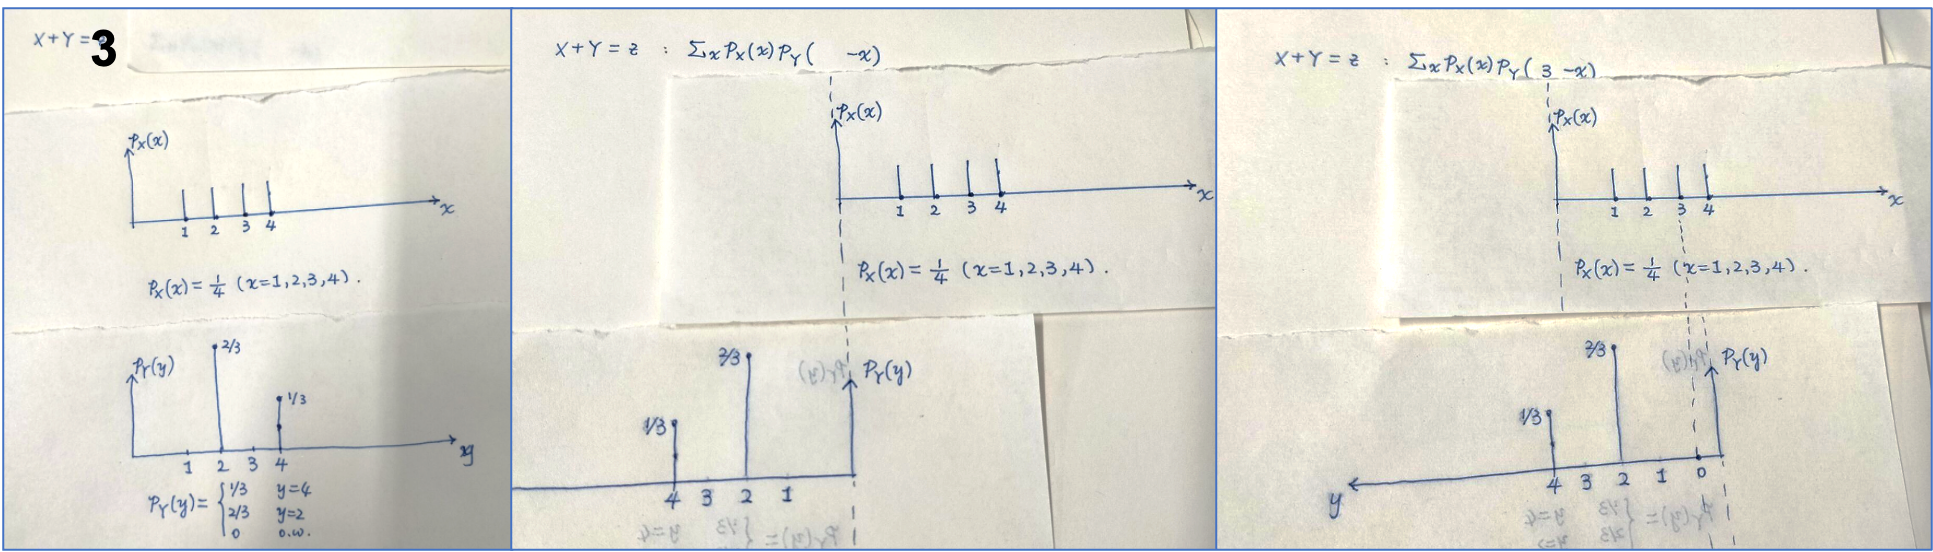
\includegraphics[width=\textwidth]{fig/ch3/convolution.png}
    \caption{直观理解卷积}
    \label{fig:convolution}
\end{figure}

\paragraph{(二)$Z=Y/X,Z=XY$的分布}

设 $(X, Y)$ 是二维连续型随机变量, 它具有概率密度 $f_{X,Y}(x, y)$.连续型随机变量$Z=Y/X$的概率密度是多少?

我们还是还是首先设出$F_{Y/X}(z)=P\{Y/X\leq z\}$. 但是这里由于函数的不连续性, 需要分两种情况: $x<0, x>0$分别考虑:

$$
\begin{aligned}
F_{Y / X}(z) & =P\{Y / X \leq z\}=\iint_{\stackrel{y / x \leq z}{x<0}} f(x, y) \mathrm{d} y \mathrm{~d} x+\iint_{\stackrel{y / x \leq z}{x>0}} f(x, y) \mathrm{d} y \mathrm{~d} x \\
& =\int_{-\infty}^0\left[\int_{z x}^{\infty} f(x, y) \mathrm{d} y\right] \mathrm{d} x+\int_0^{\infty}\left[\int_{-\infty}^{z x} f(x, y) \mathrm{d} y\right] \mathrm{d} x \\
& \varsub{y:=xu}{1cm} \int_{-\infty}^0\left[\int_z^{-\infty} x f(x, x u) \mathrm{d} u\right] \mathrm{d} x+\int_0^{\infty}\left[\int_{-\infty}^z x f(x, x u) \mathrm{d} u\right] \mathrm{d} x \\
& =\int_{-\infty}^0\left[\int_{-\infty}^z(-x) f(x, x u) \mathrm{d} u\right] \mathrm{d} x+\int_0^{\infty}\left[\int_{-\infty}^z x f(x, x u) \mathrm{d} u\right] \mathrm{d} x \\
& =\int_{-\infty}^z\left[\int_{-\infty}^+\infty|x| f(x, x u) \mathrm{d} u\right] \mathrm{d} x
\end{aligned}
$$

遵循同样的模式, 同样可以求出: $Z=XY$的概率分布. 
$$
\begin{aligned} & F_{XY}(z)=P\{XY\leq z\}\\
 & =\iint_{\substack{xy\leq z\\
 x<0}}f(x,y)\dd y\dd x+\iint_{\substack{xy\leq z\\
 x>0}}f(x,y)\dd y\dd x\\
 & =\int_{-\infty}^{0}\left(\int_{z/x}^{+\infty}f(x,y)\dd y\right)\dd x+\int_{0}^{+\infty}\left(\int_{-\infty}^{z/x}f(x,y)\dd y\right)\dd x\\
 & \varsub{y:=u/x}{1.5cm}\int_{-\infty}^{0}\left(\int_{z/x}^{+\infty}f\left(x,\frac{u}{x}\right)d\left(\frac{u}{x}\right)\right)\dd x+\int_{0}^{+\infty}\left(\int_{-\infty}^{z/x}f\left(x,\left(\frac{u}{x}\right)\dd x\right)\right)\\
 & =\int_{-\infty}^{0}\left(\left(\frac{1}{x}\right)\int_{z}^{-\infty}f\left(x,\frac{u}{x}\right)\dd u\right)\dd x+\int_{0}^{+\infty}\left(\frac{1}{x}\int_{-\infty}^{z}f\left(x,\frac{u}{x}\right)\dd u\right)\dd x\\
 & =\int_{0}^{z}\left(\int_{-\infty}^{\infty}\frac{1}{|x|}f\left(x,\frac{u}{x}\right)\dd u\right)\dd x
\end{aligned}
$$

\paragraph{(三) $M=\min \{X, Y\}$的分布}

$X, Y$ 是两个\emph{相互独立}的随机变量, 它们的分布函数分别为 $F_X(x)$ 和$F_Y(y)$.求 $M=\min \{X, Y\}$的分布函数.


   $$
\begin{aligned}
F_{\min }(z) & =P\{N \leq z\}=1-P\{N>z\} \\
& =1-P\{X>z, Y>z\}=1-P\{X>z\} \cdot P\{Y>z\}
\end{aligned}
$$

也就是
$$
F_{\min }(z)=1-\left[1-F_X(z)\right]\left[1-F_Y(z)\right] .
$$

上述的三个情况都可以推广到$n$维的情形.

\part{随机变量的数字特征}
\section{数学期望}

有这样的一个游戏: 花2元并投掷一颗均匀的骰子. 如果事件A = \{1, 2, 3\} 发生, 收到1元. 如果事件B = \{4, 5\} 发生, 收到2元. 如果事件C = \{6\} 发生, 收到6元. 你会参加这个游戏吗?

\begin{webaside}
    实际上, 真理元素的频道主实际上真的在路边做了这个实验. 可以参看他们的视频: \href{https://www.bilibili.com/video/BV1Xx411b7rM}{Bilibili: BV1Xx411b7rM}
\end{webaside}

可能我们的第一考虑是看看``平均''能得多少. 这样的随机变量$X$, \[
    X =
    \begin{cases}
    1 & \text{如果事件 A 发生} \\
    2 & \text{如果事件 B 发生} \\
    6 & \text{如果事件 C 发生}
    \end{cases}
    \]
    
    事件A、B、C的概率分别是:
    \[P(A) = \frac{3}{6}, \quad P(B) = \frac{2}{6}, \quad P(C) = \frac{1}{6}\]
    
    那么, 求结果的平均值$1 \cdot P(A) + 2 \cdot P(B) + 6 \cdot P(C)= \frac{13}{6}$.

    刚刚我们做的事情, 用更正式的语言, 实际上是就是有了一个 $(\Omega, \mathscr{A}, P)$ 这样的有限概率空间, 而 $X=X(\omega)$ 是某一随机变量, 其值域为 $\left\{x_1, \cdots, x_k\right\}$. 如果设 $A_i=\left\{\omega: X(\omega)=x_i\right\}$, 则显然 $X$ 可以表示为
    \mn{\small 下面的歌词阐述了我们在做选择的时候内心的权衡: ``可万一对了呢 ~会不会 ~我会不会更快乐 ~可万一错了呢 ~这一切 ~我是否可以承受''\\--《万一对了呢》 ChiliChill}
    $$
    X(\omega)=\sum_{i=1}^k x_i I\left(A_i\right)
    $$记 $p_i=P\left\{X=x_i\right\}$. 直观上显然: 如果在 $n$ 次独立重复试验中观测随机变量 $X$的取值, 则取 $x_i$ 的值大致应该出现 $n p_i(i=1, \cdots, k)$ 次. 
    因此, 根据 $n$ 次试验的结果, 计算的该随机变量的 ``平均值'' 大致为
    $$
    \frac{1}{n}\left[n p_1 x_1+\cdots+n p_k x_k\right]=\sum_{i=1}^k p_i x_i
    $$

    \begin{definition}[离散型随机变量的期望]
        设离散型随机变量 $X$ 的分布律为
        $$
        P\left\{X=x_k\right\}=p_k, \quad k=1,2, \cdots .
        $$
        若级数
    $$
    \sum_{k=1}^{\infty} x_k p_k
    $$
    
    绝对收敛, 则称级数 $\sum_{k=1}^{\infty} x_k p_k$ 的和为随机变量 $X$ 的数学期望, 记为 $\Ep{X}$. 即
    $$
    \Ep{X}=\sum_{k=1}^{\infty} x_k p_k
    $$
    \end{definition}

    
    仿照离散型随机变量的期望的定义, 我们同样给出连续形随机变量的定义:
    \begin{definition}{连续型随机变量的期望}
        设连续型随机变量 $X$ 的概率密度为 $f(x)$, 若积分
$$
\int_{-\infty}^{\infty} x f(x) \mathrm{d} x
$$

绝对收敛, 则称积分 $\int_{-\infty}^{\infty} x f(x) \mathrm{d} x$ 的值为随机变量 $X$ 的数学期望, 记为 $\Ep{X}$.即
$$
\Ep{X}=\int_{-\infty}^{\infty} x f(x) \mathrm{d} x
$$
    \end{definition}

    实际上, 连续型随机变量的数学期望有另一种理解. 看下面的例子: 
    \begin{example}
        \label{eg:expectation-calc}
        连续性随机变量$X\geq 0$, 其概率密度函数为$f_X(x)$. 证明$\Ep{X}=\int_0^\infty P(X>t) dt$. 
    \end{example}

    证明直接展开交换积分次序即可. 
    
    下面我们看若干常见分布的数学期望. 

    \subsection{常见分布的数学期望}

    \paragraph{Bernouli分布} 它描述的是只先进行一次事件试验, 该事件发生的概率为$p$, 不发生的概率为$1-p$. 也就是
    \begin{itemize}
        \item $P(X=1)=p$
        \item $P(X=0)=1-p$
    \end{itemize}

    因此, $ \Ep{X}=0 \cdot(1-p)+1 \cdot p=p$.

    \paragraph{Poisson分布} 它的分布是: 对于大于0的参数$\lambda$, $$
    P(X=k)=\frac{\lambda^k e^{-\lambda}}{k !}. 
    $$    

    期望的话, 就是$\sum_{i=0}^{\infty} \frac{i e^{-\lambda} \lambda^i}{i !}$. 我们可以使用《高等数学II》中的公式计算它: 
    $$
\begin{aligned}
{\E}(X) & =\lambda e^{-\lambda} \sum_{k \geq 1} \frac{1}{(k-1) !} \lambda^{k-1} & & \text { 去掉 } k=0 \text { 的那一项 } \\
& =\lambda e^{-\lambda} \sum_{j \geq 0} \frac{\lambda^j}{j !} & & \text { 变量代换 } j:=k-1 \\
& =\lambda e^{-\lambda} e^\lambda & & \text {指数函数的 Taylor 级数展开 } \\
& =\lambda & &
\end{aligned}
$$

\paragraph{几何分布}
回忆: 对与$G(X=k)$的几何分布, 表达的意思是前$k-1$次皆失败, 第$k$次成功的概率. 因此, 其概率是
    $$
    P(X=k)=(1-p)^{k-1} p
    $$

    所以它的期望表达式是: 
    $$
    \Ep{X}=\sum_{k=1}^{\infty} k p(1-p)^{k-1}
    $$

    由于$p$是常数, 我们可以把它从求和号中拿出来, 得到
    $p \sum_{k=1}^{\infty} k(1-p)^{k-1}$


\begin{itemize}
    \item 使用: $\frac{1}{1-x}  =1+x+x^2+\cdots =\sum_{k=0}^{\infty} x^k$, 当$|x|<1$时: 
    \item 两端求导: $\frac{1}{(1-x)^2}=\sum_{k=1}^{\infty} k x^{k-1}$.
    \item 令$x=1-p$, 得到$\frac{1}{p^2}=\sum_{k=1}^{\infty} k(1-p)^{k-1}$
    \item 因此期望为$1/p$.
\end{itemize}

实际上, 这个操作正是对应着它的无记忆性. 在介绍了期望的性质之后, 我们发现使用无记忆性来说明这个性质就不用如此大费周章了. 

\paragraph{均匀分布} 回顾: 均匀分布的概率密度函数$$
f(x)= \begin{cases}\frac{1}{b-a} & \text { for } a \leq x \leq b \\ 0 & \text { for } x<a \text { or } x>b\end{cases}
$$
带入计算之后, 得到了一个很平凡的结论: $$\int_a^b \frac{x}{b-a} d x=\frac{a+b}{2}.$$
这也符合直觉 -- 如果你往这里加一个支点的话, 它就会支撑起整个概率密度函数. 

\paragraph{正态分布}
回忆: 正态分布的概率密度函数$$
    f(x)=\frac{1}{\sigma \sqrt{2 \pi}} e^{-\frac{1}{2}\left(\frac{x-\mu}{\sigma}\right)^2}
    $$

    这个问题, 可以根据对称性进行求解. 注意到关于$\mu$对称.  
    $$
\frac{1}{\sqrt{2 \pi \sigma^2}} \int_{-\infty}^{\infty} x e^{-(x-\mu)^2 / 2 \sigma^2} d x=\mu
$$


    \begin{shaded}
        \paragraph{*二项分布} 它描述的是在$n$次独立重复的Bernoili试验中, 设每次试验中事件A发生的概率为$p$. 用$X$表示$n$重伯努利试验中事件A发生的{\red{次数}}.
        \mn{像这样对二项式的操作在计算机科学中是很有必要了解的. 因为我们总是在分析算法的时候用到他们. }
        其概率概率分布为$$P(X=k)={n\choose k} p^k q^{n-k}.$$
        因此
    $$
\begin{aligned}
\Ep{x}= & \teal{0} \cdot {n \choose 0} p^0(1-p)^n+\teal{1} \cdot\binom n1 p^1(1-p)^{n-1}+\cdots \\
& +\teal{(n-1)}\binom n{n-1} p^{n-1}(1-p)^1  +\teal{n}\binom nn
 p^n(1-p)^0 \\
= & \sum_{i=0}^n \teal{i}\binom ni p^i(1-p)^{n-i}
\end{aligned}
$$

我们发现它难以计算. 一个原因是里面那个青色的$i$太难受了. 如果我们能够把它去掉就好了. 幸运的是, 组合恒等式里面有这样的一条性质, 可以帮助我们完成这件事. 

回忆: 二项式系数的定义是 $\binom nk = \frac{n(n-1) \cdots(n-k+1)}{k(k-1) \cdots(1)}=\frac{n !}{k !(n-k) !}$. 其有一个有趣的等式, 可以帮助我们把东西吸收/提取出来. 也就是: 
$$
\binom rk=\frac{r}{k}\binom{r-1}{k-1} \text {, 整数 } k \neq 0
$$
这个一般形象地称为``吸收-提取恒等式''. 这个证明可以使用其定义展开即可. 
$$
\begin{aligned}
\binom rk & =\frac{r !}{k !(r-k) !} \\
& =\frac{r}{k} \cdot \frac{(r-1) !}{(k-1) !(r-k) !} \\
& =\frac{r}{k} \cdot \frac{(r-1) !}{(k-1) !((r-1)-(k-1)) !} \\
& =\frac{r}{k} \cdot \binom {r-1}{k-1}
\end{aligned}
$$


好. 有了这样的一个想法,  根据吸收-提取恒等式:
$$
\begin{aligned}
& \sum_{i=1}^n i\binom ni p^i(1-p)^{n-i} \\
= & \sum_{i=1}^n n\binom{n-1}{i-1} p^i(1-p)^{n-i} \\
= & n p \teal{\sum_{i=1}^n\binom{n-1}{i-1} p^{i-1}(1-p)^{n-i}} \\
= & n p\teal{(p+(1-p))^{n-1}}=n p
\end{aligned}
$$

这个为什么结果如此简单? 实际上因为期望有一些性质. 我们下一节会提到原因. 
    \end{shaded}

    有些分布没有数学期望. 比如Cauchy分布: $f_X(x)=\frac{4}{\pi} \frac{4}{1+x^2},-\infty<x<+\infty$. 我们在求它的积分的时候, 就会发现
    $$
\begin{aligned}
& \frac{4}{\pi} \int_{-\infty}^{\infty}|x| \frac{4}{1+x^2} \\
= & \int_0^{+\infty} \frac{2 x}{1+x^2} d x \\
= & \int_0^{+\infty} \frac{1}{1+y} d y=\ln (1+y)<+\infty .
\end{aligned}
$$发散. 因此Cauchy分布没有数学期望. 

    \subsection{数学期望的重要性质}
    
    \paragraph{1.(常数的数学期望)} 设$C$是常数, 则有$\Ep C = C.$

    事实上, 直观来看, 每一次我们得到的都一定是$C$. 因此有其合理性. 

    \paragraph{2. (常数进出数学期望)} 设$C$是常数, $X$是一个随机变量, 则有
    \[
        \Ep {CX} = C\Ep X.
    \]
    
    这是因为常数可以自由进出求和号/积分号. 

    \paragraph{3. (两个随机变量之和)}设$X,Y$是两个随机变量, 则有
    \[
        \E\left(X+Y\right) = \E\left(X\right) + \E\left(Y\right).
    \]

    事实上, 这是因为分配率得到的结果. 设二维随机变量$\left(X,Y\right)$的概率密度为$f_{X,Y}\left(x,y\right)$,其边缘概率密度为$f_X(x),f_Y(y)$
    \begin{align}
        \E\left(X+Y\right) &= \int_{-\infty}^{\infty}\int_{-\infty}^{\infty}\left(x+y\right)f_{X,Y}\left(x,y\right){d}x{d}y \notag\\
        & =  \int_{-\infty}^{\infty}\int_{-\infty}^{\infty}xf_{X,Y}(x,y){d}x{d}y + \int_{-\infty}^{\infty}\int_{-\infty}^{\infty}yf_{X,Y}(x,y){d}x{d}y \notag\\
        & = \E\left(X\right) + \E\left(Y\right)\notag.
    \end{align}

    上面的$2^\circ$和$3^\circ$合在一起被称作期望的线性性质. 这和我们在线性代数中的线性空间的理论中的一部分很相似. 

    \paragraph{4. (两个\red{独立}的随机变量之积)} 设$X,Y$是相互独立的随机变量, 则有\[
        \E\left(XY\right) = \E\left(X\right)\E\left(Y\right).
    \]



    这是因为只有独立的情况下, 联合随机变量的内容才可以得到拆开. 

    若$X$和$Y$相互独立, 
        
        \begin{align}
            \E\left(XY\right) &= \int_{-\infty}^{\infty}\int_{-\infty}^{\infty}xyf_{X,Y}\left(x,y\right){d}x{d}y = \int_{-\infty}^{\infty}\int_{-\infty}^{\infty}xyf_X\left(x\right)f_Y\left(y\right){d}x{d}y\notag\\
            & = \left[\int_{-\infty}^{\infty}xf_X\left(x\right){d}x\right]\left[\int_{-\infty}^{\infty}yf_Y\left(y\right){d}y\right] = \E\left(X\right)\E\left(Y\right).\notag
        \end{align}

    对于上面的二项分布, 我们可以注意到每一次实验, 我们都可以看做一个随机变量. 每一次的期望都是$p$, 自然, 所有的实验, 期望就是$np$. 

    \begin{exercise}
        $A, B, C, D$四人竞拍, 价高者得. 假设你是$A$, 已知$B, C, D$三人竞拍价互相独立, 切服从$U(7,11)$. 如$A$中标可以以10转让, 如何报价使得$A$获得的期望收益最大?
    \end{exercise}

    \begin{solution}
        以$G(A)$表达$A$的收益. $P(G(X)=10-X)=((x-7)/4)^3$, $P(G(X)=0)=1-((x-7)/4)^3$. 那么$\Ep{G(X)}=(10-x)(\frac{x-7} 4)^3$. 得到$x$的极值为$37/4$. 
    \end{solution}
    


    \subsection{随机变量函数的数学期望}
    下面我们来研究随机变量函数的数学期望. 

    \paragraph{1. 由随机变量$X$求$\Ep{f(X)}$} 设 $g(x)$ 是连续函数, $X$ 是随机变量.
    \begin{itemize}
        \item 如果$X$是离散型随机变量, 且分布律为 $P\left(X=x_k\right)=p_k(k=1,2, \cdots)$, 若 $\sum_k g\left(x_k\right) p_k$ 绝对收敛, 则
        $$
        \E[g(X)]=\sum_k g\left(x_k\right) p_k .
        $$
        \item 如果$X$是连续型随机变量,且概率密度函数为$f(x)$, 若$\int_{-\infty}^{+\infty} g(x)f(x)\dd x$ 绝对收敛, 则
        $$\int_{-\infty}^{+\infty} g(x)f(x)\dd x.$$
    \end{itemize}
    
    也就是只要把``系数''变为了对应的函数值. 事实上, 在对应的离散的状态下, 我们有如下的说明: 
    \begin{align*} & p_Y(y)=\sum_{\{x \mid f(x)=y\}} p_X(x) \\ & \E[f(X)]=E[Y] \\ & =\sum_y y p_Y(y) \\ & =\sum_y y \sum_{\{x \mid f(x)=y\}} p_X(x) \\ & =\sum_y \sum_{\{x \mid f(x)=y\}} y p_X(x) \\ & =\sum_y \sum_{\{x \mid f(x)=y\}} f(x) p_X(x) \\ & =\sum_x f(x) p_X(x)\end{align*}

    \paragraph{2. 用$(X,Y)$得到$\Ep{g(X,Y)}$}设$g(x,y)$为连续函数, 

    离散情形: 
    \begin{itemize}
        \item 若$(X,Y)$为离散型随机变量, 分布律为$p_{ij} = P(X=x_i,Y=y_j)(i,j=1,2,\cdots)$
        \item 且级数$\sum_i \sum_j g(x_i,y_j)p_{ij}$绝对收敛
        \item 则$$\Ep{g(X,Y)}=\sum_i \sum_j g(x_i,y_j)p_{ij}.$$
    \end{itemize}    

    连续情形:\begin{itemize}
        \item 若$(X,Y)$为连续型随机变量, 联合概率密度函数为$f(x,y)$
        \item 且积分$\int_{-\infty}^{+\infty}\int_{-\infty}^{+\infty}g(x,y)f(x,y)\dd x\dd y$绝对收敛
        \item 则$$\Ep{g(X,Y)}=\int_{-\infty}^{+\infty}\int_{-\infty}^{+\infty}g(x,y)f(x,y)\dd x\dd y.$$
    \end{itemize}  

\subsection*{多知道一点: 快速排序的期望运行时间}

我们在《算法导论》的课程上了解了如下的随机快速排序算法. 使用自然语言大概可以看做\cref{algo:quick-sort}. 
\begin{algorithm}
    \caption{随机快速排序算法}
    \label{algo:quick-sort}
    \KwIn{待排序的数组$S=[x_1, x_2, \cdots, x_n]$}
    \KwOut{排序后的数组$S$.}
    \begin{itemize}
        \item 如果$S$只有一个或者零个元素, 返回$S$. 否则继续. 
        \item 随机选择$S$中的元素$s$作为基准元素. 
        \item 把$S$分为两个小的列表$S_1, S_2$. 其中, 任何一个$S_1$中的元素比$s$要小, 任何一个$S_2$中的元素比$s$要大.
        \item 对$S_1, S_2$进行快速排序. 
        \item 返回列表$[S_1, x, S_2]$.
    \end{itemize}
\end{algorithm}

我们声称: 每一次从元素中独立地随机选取基准, 那么对于任意的输入, 快速排序比较的期望次数为$2n\lg n + O(n)$. 

\begin{proof}
    设$y_1, y_2, \cdots, y_n$是输入值$x_1, x_2, \cdots, x_n$按照升序排列的结果. 我们定义$X_{ij}(i<j)$是一个随机变量. 如果在算法执行的某一时刻$y_i$和$y_j$发生了比较, $X_{ij}$取值为1, 否则为0. 那么比较的总次数满足
    $$
    X=\sum_{i=1}^{n-1}\sum_{j=i+1}^n X_{ij}
    $$
    根据期望的线性性, $\Ep{X}=\Ep{\sum_{i=1}^{n-1}\sum_{j=i+1}^n X_{ij}}=\sum_{i=1}^{n-1}\sum_{j=i+1}^n \Ep{X_{ij}}$. 

    由于$X_{ij}$只能取0和1, 是指示变量, $\Ep{X_{ij}}$是$X_{ij}$等于1的概率. 

    什么时候$y_i$和$y_j$会发生比较呢? 我们发现$y_i$和$y_j$发生比较, 当且仅当$y_i$或$y_j$是从集合$Y_{ij}=\{y_i, y_{i+1}, \cdots, y_{j-1},y_j\}$中选取的一个基准元素. 否则, 他们会被分在不同的子列表中, 因而不会比较. 

    由于我们的基准元素是独立选取的, 因此$y_i$和$y_j$是从$Y_{ij}$中选取的一个基准元素的概率, 也就是$X_{ij}$取1的概率, 是$2/(j-i+1)$. 也就是
    $$
    \begin{aligned}
        \Ep{X}&=\sum_{i=1}^{n-1} \sum_{j=i+1}^{n} \frac 2{j-i+1}\\
        &\varsub{k:=j-i+1}{1.5cm} \sum_{i=1}^{n-1}\sum_{k=2}^{n-i+1} \frac 2k = \sum_{k=2}^n \sum_{i=1}^{n+1-k} \frac 2k \\ 
        &= \sum_{k=2}^n (n+1-k) \frac 2k = \left((n+1)\sum_{k=2}^n \frac 2k\right)-2(n-1) \\
        &= (2n+2) \sum_{k=1}^n \frac 1k - 4n.
    \end{aligned} 
    $$
\end{proof}
\section{条件数学期望}



    \begin{definition}
        设随机变量$X$在$y=y_i$的条件下的条件分布列为
        $$
        p_{i|j}=P(X=x_i | Y=y_j),
        $$
        若级数$\sum_i x_i p_{i|j}$绝对收敛, 那么称此级数$Y=Y_i$条件下$X$的条件数学期望, 记为$\Ep{X|Y=y_i}$.
    \end{definition}

    正如条件概率也是概率, 条件数学期望也是数学期望. 自然, 它就满足数学期望对应的性质. 

    \begin{example}
        有一根长度为$l$的棍子, 在$(0,l)$内均匀地取一点$X$折断. 再次在$(0,a)$选一点$Y$折断. 求$Y$的期望. 
    \end{example}

    \begin{solution}
        假设$Y$是一个具体值的情形. $\Ep{X \mid Y=y}=\frac{y}{2}$是一个数字. 但是实验之前, 这个值是随机的. 我们干脆把它写作$\Ep{X|Y}$作为一个随机变量. 其中, 记作$\Ep{X|Y}=Y/2$.
    \end{solution}



    下面来看有时候如何方便地计算期望. 我们可以把样本空间构成一组不相交的集合$A_1, A_2, \cdots, A_n$, 因此可以在每个小块上面计算期望值. 也就是: $$
    \Ep{X}=P\left(A_1\right) \Ep{X \mid A_1}+\cdots+P\left(A_n\right) \Ep{X \mid A_n} .
    $$
    这个可以使用全概率公式, 两边乘上其对应的系数得到. 这就是\textbf{全期望公式}. 


    有了这样的记号, 我们给出指数分布的期望的又一说明: 
    \begin{example}
        
    我们把原来的事件划分为不相交的两类. 
    $$
    \begin{aligned}
    & A_1:\{x=1\}, \quad A_2:\{x>1\} . \\
    & \Ep{X}=P(X=1) \Ep{X \mid x=1}+P(X>1) \Ep{X \mid x>1} .
    \end{aligned}
    $$
    那么计算它就得到了: 
    $$
\begin{aligned}
\Ep{X} & =P(X=1) E[X \mid x=1]+P(X>1) E[X \mid x>1] . \\
& =p \cdot 1+(1-p)\boxed{~~?~~}
\end{aligned}
$$
我们关注$E[X \mid x>1]$的情形, $$
\begin{aligned}
E[X \mid x-1>0] & =E[X-1 \mid x-1>0]+1 \\
& =\Ep{X}+1
\end{aligned}
$$
由于指数分布的无记忆性, 上面的式子就是$\Ep{X}+1$. 

上面的式子经过整理得到$\Ep{X}=p \cdot 1+(1-p)(\Ep{X}+1)$. 我们由此解答出来$\Ep{X}$, 因此就得到期望值为$1/p$. 

    \end{example}

    \subsection{迭代的期望}

    我们接下来考虑期望的迭代公式, 也就是$\mathbb{E}[\mathbb{E}[X \mid Y]]$. 这个符号看上去很难懂. 我们先从简单来看这个公式: 
    \begin{itemize}
        \item $\mathbb{E}[X \mid Y=y]$表示当随机变量$Y$取值$y$的时候, 随机变量$X$的期望. 
        \item 考虑所有可能的$Y$, 其构成的一组期望就是$\mathbb{E}_y[X \mid Y=y], \forall y$. 
        \item 这一组期望, 是一个关于$Y$的随机变量.为了简便,我们把这样的一组简写为$\mathbb{E}[X \mid Y]$.
        \item 对于这样的一个随机变量, 自然可以求它的期望. 
    \end{itemize}

    实际上, 这个公式有一个更简洁的表示. 我们按照定义展开: 
    $$\begin{aligned} \text{左手边} & =\int_{-\infty}^{+\infty}\left(\int_{-\infty}^{+\infty} \frac{f_{x, Y}(x, y)}{f_Y(y)} d x\right) f_Y(y) d y \\ & =\int_{-\infty}^{+\infty} \int_{-\infty}^{+\infty} x f_{x, Y}(x, y) d x d y . \\ & =\int_{-\infty}^{+\infty} x f_x(x) d x=\mathbb{E}[x]=\text{右手边}\end{aligned}$$

    这个公式有一个名字, 叫做``迭代期望定律(Law of iterated expectations)''. 

    \begin{theorem}
        迭代的期望公式:$$
\mathbb{E}[{\mathbb{E}}[X \mid Y]]=\mathbb{E}[X]
$$
    \end{theorem}

    \subsection{练习: 仅仅依赖上一个状态的Markov链}

        \begin{wrapfigure}{l}{0.4\textwidth}
        \begin{center}
            \psscalebox{0.6 0.6} % Change this value to rescale the drawing.
{
\begin{pspicture}(0,-5.46)(8.3,0.42)
\definecolor{colour0}{rgb}{0.0,0.5019608,0.0}
\definecolor{colour1}{rgb}{0.9019608,0.3019608,0.3019608}
\psframe[linecolor=black, linewidth=0.04, dimen=outer](8.3,0.14)(0.0,-5.46)
\rput[bl](3.7,-1.46){A}
\rput[bl](1.9,-4.26){B}
\rput[bl](5.2,-4.36){C}
\rput[bl](0.1,0.14){Dorm}
\psellipse[linecolor=black, linewidth=0.04, dimen=outer](3.8,-1.31)(0.7,0.65)
\psellipse[linecolor=black, linewidth=0.04, dimen=outer](2.0,-4.16)(0.7,0.7)
\psellipse[linecolor=black, linewidth=0.04, dimen=outer](5.35,-4.21)(0.65,0.65)
\rput[bl](2.3,-0.66){0.2}
\psline[linecolor=black, linewidth=0.04, arrowsize=0.05291667cm 2.0,arrowlength=1.4,arrowinset=0.0]{->}(4.3,-1.76)(5.2,-3.56)
\psline[linecolor=black, linewidth=0.04, arrowsize=0.05291667cm 2.0,arrowlength=1.4,arrowinset=0.0]{->}(3.3,-1.86)(2.2,-3.56)
\rput[bl](4.7,-2.36){0.2}
\rput[bl](2.6,-2.56){0.6}
\psline[linecolor=colour0, linewidth=0.04, arrowsize=0.05291667cm 2.0,arrowlength=1.4,arrowinset=0.0]{->}(2.5,-3.66)(3.6,-1.96)
\psline[linecolor=colour0, linewidth=0.04, arrowsize=0.05291667cm 2.0,arrowlength=1.4,arrowinset=0.0]{->}(2.7,-4.36)(4.7,-4.36)
\rput[bl](2.9,-3.06){\textcolor{colour0}{0.3}}
\rput[bl](3.4,-4.46){\textcolor{colour0}{0.7}}
\psline[linecolor=colour1, linewidth=0.04, arrowsize=0.05291667cm 2.0,arrowlength=1.4,arrowinset=0.0]{->}(5.0,-3.66)(4.1,-1.86)
\rput[bl](4.3,-2.96){\textcolor{red}{0.5}}
\rput[bl](6.7,-4.46){\textcolor{red}{0.5}}
\psbezier[linecolor=colour1, linewidth=0.04, arrowsize=0.05291667cm 2.0,arrowlength=1.4,arrowinset=0.0]{->}(5.9,-3.96)(6.7516584,-3.4359026)(7.241421,-2.8700504)(7.1,-3.86)(6.9585786,-4.8499494)(6.796546,-4.5769544)(5.8,-4.66)
\psbezier[linecolor=black, linewidth=0.04, arrowsize=0.05291667cm 2.0,arrowlength=1.4,arrowinset=0.0]{->}(3.4,-0.76)(2.9143572,0.114157274)(3.0472136,0.4344272)(2.6,-0.46)(2.1527865,-1.3544272)(2.1636708,-1.0088766)(3.1,-1.36)
\end{pspicture}
}
        \end{center}
        \caption{班主任探访的规律}
        \label{fig:meeting-supervisor-pattern}
    \end{wrapfigure}
    \paragraph{第一幕 Markov链带来的稳定分布} 有三个喜欢自学的好奇学生A,B,C. 他们整天喜欢在宿舍学习. 这自然会使他们的班主任不开心. 这就会导致班主任每天就去他们的寝室去观察, 以确保他们确实在学习. 
    
    由于他们足够观察的足够仔细, 经过一段时间的观察, 他们认为班主任会按照如\cref{fig:meeting-supervisor-pattern}这样的的规律来``探访''他们.  如果我们只看$A$同学和黑色的箭头, 其意义如下: 

    若今天班主任找$A$同学, 那么明天: 
    \begin{itemize}
        \item 0.6的概率找$B$;
        \item 0.2的概率找$C$;
        \item 0.2的概率找$A$.
    \end{itemize}

    这里一个关键的假设是: 未来的状态仅仅取决于\emph{当前状态}. 也就是$P(X_{n+1}=x|X_n=x_n)$.
    
    在这个假设下, 如果我们已知班主任老师第一天找$B$, 第二天找$A$, 那么请问, 第三天找$C$的概率为多大? 按照我们刚刚的假设, 第三天找谁只与第二天有关. 因此第二天找了$A$, 自然第三天找$C$的概率为0.2. 

    自然, 日子一天天的过去, 他们想知道从长期来看, 班主任来``探访''他们的概率是多少. 比如, 他们记录了10天以内班主任的行踪轨迹: 
    $$
    A \to B \to A\to C \to A \to C\to C\to C\to A\to B.
    $$

    在这10天里面, $P(A\text{被找到}), P(B\text{被找到}),P(C\text{被找到})$的概率分别为4/10, 2/10, 4/10. 因此, 他们面临的第一个问题就是在前$n$天($n\to \infty$)的时候期望的结果是多少. 

    事实上, 上面的状态转换关系是一个图. 可以用$3\times 3$的矩阵表示如下(第一行和第一列为标示,$M[C][B]$表示第一天老师在$C$, 第二天去$B$的概率.):   
    $$
M=\left[\begin{array}{cccc}
&\text { A } & \text {B} & \text {C} \\
\text{A}&0.2 & 0.6 & 0.2 \\
\text{B}&0.3 & 0 & 0.7 \\
\text{C}& 0.5 & 0 & 0.5
\end{array}\right]
$$以及最初的状态(比如找了B, 初始状态用$1\times 3$的矩阵表示为$
\pi_0=\left[\begin{array}{ccc}
\text{A} & \text{B} & \text {C} \\
0 & 1 & 0
\end{array}\right]
$)若达到了稳定状态, 意味着找到这样的一个$\pi$, 使得$\pi A=\pi$. 这就是矩阵的特征向量.在这个情况下, 这个稳定的$\pi$为$\pi=\left[\frac{25}{71}, \frac{15}{71}, \frac{31}{71}\right]$.

为什么这样是对的呢? 我们考虑到达了状态$j$,从$i$状态开始,在 $n$ 步后, 定义为$P_{ij}(n)$. 同样如果我们有一个矩阵$$
M=\left[\begin{array}{ccc}
A_{11} & A_{12} & A_{13} \\ 
A_{21} & A_{22} & A_{23} \\ 
A_{31} & A_{32} & A_{33} \\ 
\end{array}\right]
$$
那么用一步从0到达2只有一种可能的情况:$P_{02}(1)=A_{02}$.  两步从0到2到达的一种情况就要分情况了. 
$$
\begin{aligned}
 P_{02}(2)&=A_{01} \times A_{12}+A_{00} \times A_{02}+A_{02} \times A_{22} \\
=& \left[\begin{array}{lll}
A_{00} & A_{01} & A_{02}
\end{array}\right] \times\left[\begin{array}{l}
A_{02} \\
A_{12} \\
A_{22}
\end{array}\right] \\
&
\end{aligned}
$$
类似的, 有$$
P_{10}(2)=\left[\begin{array}{lll}
A_{10} & A_{11} & A_{12}
\end{array}\right] \times\left[\begin{array}{c}
A_{00} \\
A_{10} \\
A_{20}
\end{array}\right]
$$
把每个状态都列举一遍, 我们就可以使用矩阵乘法. 也就是$$
P(2)=A^2=\left[\begin{array}{ccc}
0.5 & 0.2 & 0.3 \\
0.6 & 0.2 & 0.2 \\
0.1 & 0.8 & 0.1
\end{array}\right] \times\left[\begin{array}{ccc}
0.5 & 0.2 & 0.3 \\
0.6 & 0.2 & 0.2 \\
0.1 & 0.8 & 0.1
\end{array}\right]
$$也就是$P_{i_j}(n)=A_{i j}^n$. 

\paragraph{第二幕 Markov链的期望时间} 现在, 他们摸清楚了每一次他们老师来的模式. 
现在他们的想法是...
\section{期望相关的不等式}

\paragraph{1. Jensen不等式} 先从一个简单的例子开始. 假设我们从$[1,99]$的范围内选取一个正方形的边长$X$, 问面积的期望是多少? 根据上面的公式, 我们知道$\Ep{X^2}= \int_{0}^{99} x^2 dx = 9950/3$. 

在式子变得复杂之后, 这样的运算就稍显麻烦. 能不能偷懒计算$\Ep{X}^2$代替上述的计算? 并不可以, 因为$\Ep{X}^2=50^2=2500.$ 但是我们可以看到大小关系: $\Ep{X^2}\geq \Ep{X}^2$. 并且可以证明它是对的: 
\begin{proof}
    考虑$Y=(X-\Ep{X})^2$, 随机变量$Y$非负, 意味着其期望也是非负的. 所以有
    $$
\begin{aligned}
0 \leq \mathbb{E}[Y] & =\mathbb{E}\left[(X-\mathbb{E}[X])^2\right] \\
& =\mathbb{E}\left[X^2-2 X \mathbb{E}[X]+(\mathbb{E}[X])^2\right] \\
& =\mathbb{E}\left[X^2\right]-2 \mathbb{E}[X \mathbb{E}[X]]+(\mathbb{E}[X])^2 \\
& =\mathbb{E}\left[X^2\right]-(\mathbb{E}[X])^2
\end{aligned}
$$
\end{proof}

\mn{-- 高数老师告诉过我, 高等数学里面和数学分析里面函数的凹凸性定义是相反的. 求偏导的时候求的顺序也是相反的. 那我应该相信谁?  \\ -- 相信定义. }
实际上, 这只是Jensen不等式的一个例子. Jensen不等式会告诉我们, 对于任意的一个凸函数$f$, 都会有$\Ep{f(X)}\geq f(\Ep{X})$. 

\begin{asidebox}
回顾凸函数: 一个函数$f:\mathbb R \to \mathbb R$是凸函数, 当且仅当$\forall x_1, x_2, 0\leq \lambda \leq 1$, 有$$
f\left(\lambda x_1+(1-\lambda) x_2\right) \leq \lambda f\left(x_1\right)+(1-\lambda) f\left(x_2\right) .
$$

并且我们知道, 如果 $f$ 是二次可微函数, 则 $f$ 是凸函数当且仅当 $f''(x)\geq 0$. 
\end{asidebox}

\begin{theorem}
    如果$f$是凸函数, 那么$\mathbb{E}[f(X)] \geq f(\mathbb{E}[X])$. 
\end{theorem}

\begin{proof}
    假设 $f$ 有Taylor 展开式. 令 $\mu=\mathbb{E}[X]$. 根据Taylor中值定理,存在一个值 $c$ 使得
$$
\begin{aligned}
f(x) & =f(\mu)+f^{\prime}(\mu)(x-\mu)+\frac{f^{\prime \prime}(c)(x-\mu)^2}{2} \\
& \geq f(\mu)+f^{\prime}(\mu)(x-\mu)
\end{aligned}
$$
由于$f$是凸函数, 得到 $f^{\prime \prime}(c)>0$ . 两边同时取期望, 得到: 
$$
\begin{aligned}
\mathbb{E}[f(X)] & \geq \mathbb{E}\left[f(\mu)+f^{\prime}(\mu)(X-\mu)\right] \\
& =\mathbb{E}[f(\mu)]+f^{\prime}(\mu)(\mathbb{E}[X]-\mu) \\
& =f(\mu)=f(\mathbb{E}[X]) .
\end{aligned}
$$
\end{proof}

\paragraph{2. Cauchy-Schwarz不等式}
这个不等式说的是下面的一个事情: 


\mn{这使我想到了线性代数的时候学习内积空间的时候的痛苦... }
对于随机变量  $ X, Y $, 我们有$ \mathbb{E}[|X Y|]^2 \leq \mathbb{E}\left[X^2\right] \mathbb{E}\left[Y^2\right]$
    
  
    
    首先考虑$\Ep{X^2} = \int_{-\infty}^{\infty} x^2 f_X(x), \Ep{X^2} = \int_{-\infty}^{\infty} y^2 f_Y(y)$. 为了方便起见, 不妨设$\Ep{X}, \Ep{Y}$都大于0. 假若我们引入新变量, 使得我们的$\tilde{X}, \tilde{Y}$的值都在 0到1之间: 
    $$
    \tilde{X}:= \frac{X}{\sqrt{\Ep{X^2}}},\tilde{Y}:= \frac{Y}{\sqrt{\Ep{Y^2}}} 
    $$
    这个时候由于任意的值有基本不等式, 故随机变量也要满足基本不等式描述的: $2|\tilde{X}\tilde{Y}|\leq \tilde{X^2}\tilde{Y^2}$. 对两边取期望, 有$2\Ep{\tilde{X}\tilde{Y}}\leq \Ep{\tilde{X^2}}\Ep{\tilde{Y^2}}=2$. 因此有$\Ep{\tilde{X}\tilde{Y}}\leq 1$, 自然
    $$
        \Ep{|X Y|}^2 = \mathbb{E}\left[X^2\right] \mathbb{E}\left[Y^2\right]
    $$ 

    \begin{asidebox}
        这个不等式我们在线性代数课程上面讲解向量的模的时候也有一个类似的不等式. 也就是如果一个线性空间$V$中$u,v\in V$, 那么有
        $$
        |\langle u, v\rangle| \leq\|u\|\|v\|.
        $$
        其中, $||\cdot||$是$\cdot$的范数. 

        向量的范数一般定义为$\sqrt{\langle v, v\rangle}$. 
    \end{asidebox}

\paragraph{3. Markov不等式} 概率和期望之间有什么联系? 在\cref{eg:expectation-calc}中, 我们了解到了期望计算和概率相联系的一种形式: $\Ep{X}=\int_0^\infty P(X>t) dt$. 自然的, $P(X>\epsilon)$和$\Ep{X}$有联系. 

\begin{theorem}
    Markov不等式: 
    $$
\forall \varepsilon>0, P(X>\varepsilon) \leq \frac{\mathbb{E}[X]}{\varepsilon}
$$
\end{theorem}

\begin{wrapfigure}{l}{0.6\textwidth}
    % \usepackage[usenames,dvipsnames]{pstricks}
% \usepackage{pstricks-add}
% \usepackage{epsfig}
% \usepackage{pst-grad} % For gradients
% \usepackage{pst-plot} % For axes
% \usepackage[space]{grffile} % For spaces in paths
% \usepackage{etoolbox} % For spaces in paths
% \makeatletter % For spaces in paths
% \patchcmd\Gread@eps{\@inputcheck#1 }{\@inputcheck"#1"\relax}{}{}
% \makeatother
% 
\psscalebox{0.6 0.6} % Change this value to rescale the drawing.
{
\begin{pspicture}(0,-2.5666666)(2.715555,2.5666666)
\definecolor{colour0}{rgb}{0.8,0.8,0.8}
\definecolor{colour1}{rgb}{1.0,0.7019608,0.6}
\rput(1.4555556,-0.36666676){\psaxes[linecolor=black, linewidth=0.04, arrowsize=0.05291667cm 2.0,arrowlength=1.4,arrowinset=0.0, tickstyle=full, axesstyle=axes, labels=all, ticks=all, ticksize=0.1411111cm, dx=1.0cm, dy=1.0cm]{<->}(0,0)(0,0)(8,2)}
\rput[bl](0.15555556,2.0333333){$y=P(x>t)$}
\rput[bl](9.555555,-1.1666667){$t$}
\pscustom[linecolor=black, linewidth=0.04]
{
\newpath
\moveto(1.4555556,0.5333333)
\lineto(2.0813131,0.4)
\curveto(2.394192,0.33333328)(3.3328283,0.2)(3.9585857,0.13333328)
\curveto(4.5843434,0.066666566)(7.2214646,-0.066666566)(9.232828,-0.13333343)
}
\pspolygon[linecolor=black, linewidth=0.04, fillstyle=gradient, gradlines=2000, gradbegin=colour0, gradend=colour1](1.4555556,0.43333322)(1.4555556,-0.36666676)(9.255555,-0.36666676)(9.255555,-0.16666676)(5.4555554,0.03333323)(3.4555554,0.13333324)(1.9555556,0.43333322)(1.4555556,0.53333324)(1.4555556,0.53333324)(1.4555556,0.53333324)
\psline[linecolor=black, linewidth=0.04, arrowsize=0.05291667cm 2.0,arrowlength=1.4,arrowinset=0.0]{->}(4.9555554,-0.26666677)(5.3555555,-1.0666667)
\rput[bl](5.2555556,-1.6666667){$E(X)=\int_0^{+\infty}P(X>t)dt$}
\psline[linecolor=black, linewidth=0.04, arrowsize=0.05291667cm 2.0,arrowlength=1.4,arrowinset=0.0]{->}(2.9555554,0.2385964)(2.9555554,-2.0614035)(2.9555554,-2.1614037)
\rput[bl](2.8555555,-2.5666668){$\epsilon$}
\psline[linecolor=black, linewidth=0.04, linestyle=dashed, dash=0.17638889cm 0.10583334cm](2.9555554,0.23333323)(1.4555556,0.23333323)(1.4555556,0.23333323)
\psframe[linecolor=black, linewidth=0.04, linestyle=dashed, dash=0.17638889cm 0.10583334cm, dimen=outer](0.02,2.5666666)(0.0,2.5466666)
\psframe[linecolor=black, linewidth=0.04, linestyle=dashed, dash=0.17638889cm 0.10583334cm, dimen=outer](0.02,2.5666666)(0.0,2.5466666)
\psframe[linecolor=blue, linewidth=0.04, linestyle=dashed, dash=0.17638889cm 0.10583334cm, fillstyle=crosshatch, hatchwidth=0.028222222, hatchangle=0.0, hatchsep=0.1411111, dimen=outer](2.9555554,0.23333323)(1.4555556,-0.36666676)
\end{pspicture}
}
 
    \caption{Markov不等式限制的方式}
    \label{fig:markov-ineq}
\end{wrapfigure}


\mn{-- 怎么说把这个东西切了就切了? 有点太粗暴了吧! \\ -- 实际上期望是它的一阶矩, 如果我们知道了更高阶的矩, 我们得到的信息就多了. }
我们采用最粗暴的限制限制手段. 如\cref{fig:markov-ineq}, 仅仅考虑$0\leq t\leq \epsilon, 0<y<P(x>\epsilon)$的部分. 因此, 我们可以得到证明: 
$$
\begin{aligned}
\mathbb{E}[x] & \geq \int_0^{\varepsilon} P(x>t) d t \\
& \geq \int_0^{\varepsilon} P(x>\varepsilon) d t \\
& =\varepsilon P(x>\varepsilon)
\end{aligned}
$$

于是我们可以得到想要的不等式. 

\section*{练习题: 数学期望}

\begin{exercise}
    某个大楼有10层, 某次有25人在一楼搭乘电梯上楼. 假设每人都等可能地在2到10层中的任何一层出电梯, 并且出电梯与否互相独立. 同时在2到10层中没有人上电梯. 并且电梯只有在有人要出电梯的时候才停止. 求电梯停下的总次数的数学期望. 
\end{exercise}

\begin{solution*}
每个人在第$i$层下的概率为$P_i=1/9, i=1,2,\cdots, 10$. 记第$k$个人在第$i$层下电梯记作$A_{k,i}$. 那么对于任意的$i$, $P(A_k)=1/9, P(\overline{A_k})=8/9. (k=1,2,\cdots, 25)$. 又因为$A_{1, i}, \cdots, A_{25, i}$相互独立, 那么第$i$层无人下电梯的概率为
$$
P\left(\prod_{i=1}^{25} \overline{A_k}\right) = \prod_{i=1}^{25}P\left(\overline{A_k}\right) = \left(\frac89\right), (k=1,2,\cdots, 25).
$$

设$X_i$是指示第$i$层有没有人下的示性函数, 那么, $P(X=0)=(8/9)^{25}$, $P(X=1)=1-(8/9)^{25}$.

因此电梯停的总次数为$X=\sum_{i=2}^{10}X_i=9\times\left(1-(8/9)^{25}\right)$
\end{solution*}

\begin{exercise}
    设随机变量$X,Y$相互独立, 且都服从$N(\mu, \sigma^2)$. 设$Z=\max\{X,Y\}$. 求$\Ep{Z}$.
\end{exercise}

\begin{solution*}
    正则化变量. 令$U:=\frac{X-\mu}{\sigma}, V:=\frac{Y-\mu}{\sigma}$. 那么$X=\sigma U+\mu, Y=\sigma V+\mu$. 由于$X,Y$独立, 因此$U,V$独立. 且 $U \sim N(0,1), V \sim N(0,1)$. 发现$Z=\max \{X, Y\}=\max \{\sigma U+\mu, \sigma V+\mu\}=\sigma \max (U, V)+\mu$.

    要求$\max (U, V)=\frac{1}{2}(U+V+|U-V|)$, 我们要知道$|U-V|$的分布. 令$T:=U-V \sim N(0,2)$. 考虑$$E(|T|)=\int_{-\infty}^{+\infty}|t| \frac{1}{\sqrt{2 \pi} \cdot \sqrt{2}} e^{-\frac{t^2}{2 \times 2}} d t=\frac{2}{\sqrt{\pi}}.$$ 因此得到$E[\max (U, V)]=\frac{1}{2}(E U+E V+E|U-V|)=\frac{1}{\sqrt{\pi}}$. 从而$E[\max \{X, Y\}]=\sigma E[\max (U, V)]+\mu=\frac{\sigma}{\sqrt{\pi}}+\mu$. 
\end{solution*}

\begin{exercise}
    对于任意的整数$k>1$, 证明$\Ep{X^k}\geq (\Ep{X})^k$.
\end{exercise}

\begin{solution*}
    使用Jensen不等式. 令$f(x):=x^n$. 
\end{solution*}

\begin{exercise}
    (负二项分布) 现在考虑投掷一枚硬币, 直到第$k$次出现正面的投掷次数的$X$的分布. 其中每次投掷硬币出现是独立的, 概率为$p$. 证明: 对于$n>k$, 这个分布是
    $$
    P(X=n) = \binom{n-1}{k-1}p^k(1-p)^k.
    $$
\end{exercise}

\begin{solution*}
    可以考虑在出现最后一次正面之前, 我们需要在$n-1$个空格里面插入$k-1$个正面. 其余的是反面. 由此可以得到这个等式的意义. 
\end{solution*}

\begin{exercise}
    对于一枚每次投出正面的概率是$p$的硬币, 每次投掷之间互相独立, 直到第$k$次正面出现的时候, 期望的投掷次数是多少? 
\end{exercise}

\begin{solution*}

    方法1. 令$\Ep{N_k}:=$有$n$个正面投掷的期望数. 令$X_1$是第一次投掷的结果. 如果第一次的结果是反面, 那么还会回到$N_k$, 但是期望会加1. 反之, 就会到达$N_{k-1}$, 同样期望会加一. 也就是
    $$
\Ep{N_k \mid X_1=T}=1+\Ep{N_k}
$$
$$
\Ep{N_k \mid X_1=H}=1+E\left[N_{k-1}\right]
$$

因此有表达式$\Ep{N_k}=\Ep{N_k \mid X_1=H} \cdot P\left(X_1=H\right)+\Ep{N_k \mid X_1=T} \cdot P\left(X_1=T\right)$. 解之, 得到$\Ep{N_k}=\Ep{N_{k-1}}+\frac{1}{p}$. 因此是 $\Ep{N_k}=n/p$.

    高中生: 考虑$f_i$代表现在已经扔出了$i$个正面, 还需要扔的期望数. 根据这个定义$f_k=0$, $f_{k-1}=(1-p)(f_{k-1}+1)+p(f_k+1)$. 

\end{solution*}


\begin{exercise}
    我们在一个$n$张不同的卡牌中进行带放回的抽卡, 抽出每一张卡的概率相等. 请问我们期望抽取多少次, 才能把所有的卡牌见到一遍? 
\end{exercise}

\begin{solution*}
    可以考虑当前已经见到了$k$个卡牌, 那么还有$k/n$的概率回到当前的状态, $(n-k)/n$的概率到达见到的少一个的状态. 
\end{solution*}

\begin{exercise}
    我们一遍一遍地投掷一个均匀的筛子. 在连续出现两个6之前, 期望的投掷次数是多少? (答案不是36).
\end{exercise}
\begin{solution*}
    想办法搞明白各个你的划分之间的转移关系. 或者看Markov链的相关内容. 
\end{solution*}


\begin{exercise}
     数字$1,2,\cdots, n$可以用如下的排列函数$\pi:[1..n] \to [1..n]$表示. 其中, $\pi(i)$是$i$在这个排列中的序号. 排列$\pi$的不动点是满足$\pi(x)=x$的$x$的集合. 求从所有排列中选取一个排列的不动点的期望. 
\end{exercise}

\begin{solution*}
    一个简单的方法: 定义$f(\sigma)$ 为随机一个排列$\sigma$的不动点的数量. 
    那么$$
    \mathbb{E}[{f}(\sigma)]=\mathbb{E}\left[\sum_{{i}=1}^{{n}} \mathbf{1}_{\sigma({i})={i}}\right]=\sum_{{i}=1}^{{n}} \mathbb{E}\left[1_{\sigma({i})={i}}\right]
    $$
    对于每个$i$,$i$ 成为 $\sigma$ 的一个不动点的概率等于 $\sigma(i)$ 等于 $i$ 的概率,因此等于 $\frac{1}{n}$。利用这个结果,我们得到 $\mathbb{E}[f(\sigma)]=1$。
\end{solution*}

\begin{exercise}
    假设 $a_1, a_2, \dots, a_n$ 是 {1, 2, $\dots$, $n$} 的一个随机排列,等可能地是 $n!$ 种可能的排列之一。当对列表 $a_1, a_2, \dots, a_n$ 进行排序时,元素 $a_i$ 必须移动 $|a_i - i|$ 个位置才能到达其在排序后的位置。求出$$
    \mathbb{E}\left[\sum_{i=1}^n\left|a_i-i\right|\right]
    $$
    也就是元素移动的期望总距离. 
\end{exercise}

\begin{solution*}
    和上面一样, 使用期望的线性性. 
\end{solution*}

\begin{exercise}
    排列 $\pi: [1, n] \rightarrow [1, n]$ 可以表示为一张图. 我们可以这样做: 为每个数字 $i, i = 1, \dots, n$ 设立一个顶点。如果排列将数字 $i$ 映射到数字 $\pi(i)$,则从顶点 $i$ 到顶点 $\pi(i)$ 绘制一个有向边。这导致一个由不相交环构成的图。注意,其中一些环可能是自环。在 $n$ 个数字的随机排列中,期望的环的数量是多少?
\end{exercise}

\begin{solution*}
    设 $h(n)$ 为 [n] 的随机排列中环的平均数;我声称 $h$ 满足以下递推关系:$h(n)=\frac{n-1}{n}h(n-1)+\frac{1}{n}(h(n-1)+1)$。因为:
    设 $\pi$ 是 {2,3,…,$n$} 的任意排列,用环形式表示。假设忽略括号,从左到右排列的 $\pi$ 的条目是 $\pi_1,\dots,\pi_{n-1}$。现在,在 $\pi$ 中以以下两种方式之一插入 $1$。
    \begin{itemize}
        \item 在 $\pi_1$ 的左边作为 $(1)$,形成一个独立的环。
        \item 立即在 $\pi_k$ 的某个 $k=1,\dots,n-1$ 的位置之后插入,与 $\pi_k$ 同一个环中。
    \end{itemize}
    每个 $[n]$ 的排列都可以唯一地通过这种方式从 {2,…,$n$} 的一个唯一排列 $\pi$ 获得。

一个 {2,…,$n$} 的随机排列的平均环的数量当然是 $h(n-1)$。递推关系 (1) 立即由以下事实推出:上述操作 (1) 增加了 $1$ 个环,并占据了所有情况中的 $\frac{1}{n}$,而操作 (2) 不改变环的数量,并占据了剩余的 $\frac{n-1}{n}$ 情况。

计算可知, 
$$
h(n)=H_n=\sum_{k=1}^n \frac{1}{k} \text {. }
$$
\end{solution*}
\section{方差}
随机变量 $X$ 的方差, 表征 $X$ 取值的散布程度. 最简单的想法是: 可以使用$\Ep{|X-\Ep{X}|}$来表征. 但是, 由于带着绝对值在求导的时候会带来不少麻烦, 我们考虑使用平方来操作, 也就是$\Ep{(X-\Ep{X})^2}$. 

\begin{definition}
    定义 设 $X$ 是一个随机变量, 若 $E\left\{[X-E(X)]^2\right\}$ 存在, 则称 $\Ep{(X-\Ep{x})^2}$ 为 $X$ 的方差, 记为 $D(X)$ 或 $\operatorname{Var}(X)$, 即
$$
D(X)=\operatorname{Var}(X):=\Ep{(X-\Ep{X})^2}.
$$
\end{definition}

在应用上还引入量 $\sqrt{D(X)}$, 记为 $\sigma(X)$, 称为标准差或均方差.

其实际意义是明显的: 我们查看方差的大小
\begin{itemize}
    \item $D(X)$ 较小:  $X$ 的取值比较集中在 $\Ep X $ 的附近
    \item $D(X)$ 较大: 表示 $X$ 的取值较分散.
\end{itemize}

其实, 方差说特别也不特别, 它实际上就是随机变量 $X$ 的函数 $g(X)=(X-E(X))^2$的期望. 

对这个式子做一些简单的化简, 我们发现, 要计算一个数的方差, 我们只需要计算$\Ep{X}$以及$\Ep{X^2}$即可. 

   \begin{proposition}
       随机变量 $X$ 的方差可按下列公式计算.
   $$
   D(X)=E\left(X^2\right)-[E(X)]^2 .
   $$
   \end{proposition}
   
   其证明如下: 
   \begin{proof}
       由数学期望的性质 $1^{\circ}, 2^{\circ}, 3^{\circ}$ 得
   $$
   \begin{aligned}
   D(X) & =E\left\{[X-E(X)]^2\right\}=E\left\{X^2-2 X E(X)+[E(X)]^2\right\} \\
   & =E\left(X^2\right)-2 E(X) E(X)+[E(X)]^2 \\
   & =E\left(X^2\right)-[E(X)]^2 .
   \end{aligned}
   $$
      \end{proof}




   \subsection{方差的性质}

   我们首先从抽象的层面说明方差具有哪些性质. 实际上, 这只是个关于期望的性质的练习 -- 方差只是求解一堆数学期望而已. 我们先假设下面所遇到的随机变量其方差存在: 

   \paragraph{1. 常数的方差是0} 设 $C$ 是常数, 则 $D(C)=0$.
   \begin{proof}
    代入定义,有 $D(C)=E\left\{[C-E(C)]^2\right\}=0$.
   \end{proof}


   \paragraph{2. 一个变量的线性变换后的方差} 设 $X$ 是随机变量, $C$ 是常数, 则有
   $$
   D(C X)=C^2 D(X), \quad D(X+C)=D(X) .
   $$

   \begin{proof}
    
    $$
\begin{aligned}
D(C X) & =E\left\{[C X-E(C X)]^2\right\}=C^2 E\left\{[X-E(X)]^2\right\}=C^2 D(X) \\
D(X+C) & =E\left\{[X+C-E(X+C)]^2\right\}=E\left\{[X-E(X)]^2\right\}=D(X)
\end{aligned}
$$
   \end{proof}

   \paragraph{3. 两个随机变量和的方差} 设 $X, Y$ 是两个随机变量, 则有\mn{可不要忘记了这个2. !}
   $$
   D(X+Y)=D(X)+D(Y)+2 E\{(X-E(X))(Y-E(Y))\} .
   $$
   
   特别, 若 $X, Y$ 相互独立, 则有
   $$
   D(X+Y)=D(X)+D(Y) .
   $$
   
   这一性质可以推广到任意有限多个相互独立的随机变量之和的情况.

   \begin{proof}
    $$
\begin{aligned}
D(X+Y)= & E\left\{[(X+Y)-E(X+Y)]^2\right\} \\
= & E\left\{[(X-E(X))+(Y-E(Y))]^2\right\} \\
= & E\left\{(X-E(X))^2\right\}+E\left\{(Y-E(Y))^2\right\} \\
& +2 E\{[(X-E(X)][Y-E(Y)]\} \\
= & D(X)+D(Y)+2 E\{[X-E(X)][Y-E(Y)]\} .
\end{aligned}
$$

对于其中的$ E\{[(X-E(X)][Y-E(Y)]\}$一项: $$
\begin{aligned}
& 2 E\{[(X-E(X)][Y-E(Y)]\} \\
& =2 E\{X Y-X E(Y)-Y E(X)+E(X) E(Y)\} \\
& =2\{E(X Y)-E(X) E(Y)-E(Y) E(X)+E(X) E(Y)\} \\
& =2\{E(X Y)-E(X) E(Y)\} .
\end{aligned}
$$
   \end{proof}

   

    \subsection{常见分布的方差}
    \paragraph{1. 均匀分布} 由于期望$\Ep{X}$我们已经求过了, 我们来看平方的期望$\Ep{X^2}$. 经过简单的计算, 我们发现$$
    E\left(X^2\right)=\int_{-\infty}^{\infty} x^2 f(x) d x=\frac{b^2+a b+a^2}{3}
    $$
    
    因此
    $$
    D(X)=E\left(X^2\right)-E(X)^2=\frac{(b-a)^2}{12}.
    $$

    \paragraph{2. Poisson 分布} 我们回忆参数为$\lambda$的Poisson分布的概率分布是$f(k )=\frac{e^{-\lambda} \lambda^k}{k !}$. 同样的, 
    $$
    \begin{aligned}
    E\left(X^2\right) & =\sum_{k=0}^{\infty} k^2 \frac{\lambda^k e^{-\lambda}}{k !}=\sum_{k=1}^{\infty} k e^{-\lambda} \lambda \frac{\lambda^{k-1}}{(k-1) !} \\
    & =\sum_{k=1}^{\infty}(k-1+1) \lambda e^{-\lambda} \frac{\lambda^{k-1}}{(k-1) !} \\
    & =\sum_{k=1}^{\infty}(k-1) \lambda e^{-\lambda} \frac{\lambda^{k-1}}{(k-1) !}+\lambda e^{-\lambda} \sum_{k=1}^{\infty} \frac{\lambda^{k-1}}{(k-1) !} \\
    & =\lambda^2 e^{-\lambda} \sum_{k=2}^{\infty} \frac{\lambda^{k-2}}{(k-2) !}+\lambda \\
    & =\lambda^2+\lambda \\
    D(X) & =\lambda^2+\lambda-\lambda^2=\lambda
    \end{aligned}
    $$

    \paragraph{3. 指数分布} 回忆它的概率分布函数为$$
    f(x)=\lambda e^{-\lambda x}, x \geq 0
    $$并且$\Ep{X}=1/\lambda$. 我们还是关注$\Ep{X^2}$. 
    $$
\begin{aligned}
E X^2 & =\int_0^{+\infty} x^2 \lambda e^{-\lambda x} d x \\
& =-\int_0^{+\infty} x^2 d e^{-\lambda x}=-\left.x^2 e^{-\lambda x}\right|_0 ^{+\infty}+\int_0^{+\infty} 2 x e^{-\lambda x} d x 
\end{aligned}
$$

因此
$$
\operatorname{Var}(\mathrm{X})=E X^2-(E X)^2=\frac{1}{\lambda^2}
$$

\paragraph{4. 正态分布} 我们发现正态分布的通用表达式比较麻烦. 我们首先计算标准正态分布的方差, 然后试图通过线性变换的方法得到原来的正态分布表达式. 回忆$N(0,1)=\varphi(x)=\frac{1}{\sqrt{2 \pi}} e^{-\frac{x^2}{2}}$. 

计算的大概过程大概如下: 
\begin{itemize}
    \item 写出表达式: $E\left(X^2\right)=\int_{-\infty}^{+\infty} \frac{1}{\sqrt{2 \pi}} x^2 e^{-\frac{x^2}{2}} d x$
    \item 由于是偶函数, $E\left(X^2\right)=2 \int_0^{+\infty} \frac{1}{\sqrt{2 \pi}} x^2 e^{-\frac{x^2}{2}} d x$
    \item 希望计算出$\int_0^{+\infty} \frac{1}{\sqrt{2 \pi}} x^2 e^{-\frac{x^2}{2}} d x$.
    \item 极坐标换元, 得到值为$1/2$.
    \item 因此$\Ep{X^2}=1$.
    \item $D(X)=E\left(X^2\right)-(E(X))^2=1-0^2=1$
    \item 通过标准化得到方差
\end{itemize}

接着我们做线性变换代换回去. 
$$
\begin{aligned}
& X \sim N\left(\mu, \sigma^2\right), Z \sim N(0,1) \\
& Z=\frac{X-\mu}{\sigma} \sim N(0,1) \\
& D(Z)=D\left(\frac{X-\mu}{\sigma}\right)=D\left(\frac{X}{\sigma}-\frac{\mu}{\sigma}\right)=D\left(\frac{X}{\sigma}\right)=\frac{1}{\sigma^2} D(X)=1
\end{aligned}
$$
得到$D(x)=\sigma^2$.

\paragraph{5. 几何分布 } 我们回忆其分布函数为$P(X=k)=(1-p)^{k-1} p$ $\frac{1}{p}$, 以及$\Ep X=1/p$. 方便起见, 令$q:=1-p$. 

那么
$$\begin{aligned} D(X) & =E\left(X^2\right)-(E(X))^2 \\ & =\sum_{k=1}^{\infty} k^2 q^{k-1} p-\frac{1}{p^2} \\ & =p\left[\sum_{k=1}^{\infty}(k+1) k q^{k-1}-\sum_{k=1}^{\infty} k q^{k-1}\right]-\frac{1}{p^2} \\ & =p\left(\frac{\mathrm{d}^2}{\mathrm{~d} q^2} \sum_{k=1}^{\infty} q^{k+1}-\frac{\mathrm{d}}{\mathrm{d} q} \sum_{k=1}^{\infty} q^k\right)-\frac{1}{p^2} \\ & =p\left[\frac{2}{(1-q)^3}-\frac{1}{(1-q)^2}\right]-\frac{1}{p^2}=\frac{q}{p^2} .\end{aligned}$$

\paragraph{6. 二项分布} 
我们在上一节里面用非常痛苦的方法求解了它的期望. 这里, 我们还是先不用任何的性质, 再来痛苦地求解一下它的方差. 

$$\begin{aligned} E\left(k^2\right) & =\sum_{k=0}^n k^2 p(k) \\ & =\sum_{k=1}^n k^2\left(\begin{array}{l}n \\ k\end{array}\right) p^k q^{n-k} \\ & =\sum_{k=1}^n[{k}({k}-1)+{k}]\left(\begin{array}{l}n \\ k\end{array}\right) p^k q^{n-k} \\ & =\sum_{k=1}^n k(k-1)\left(\begin{array}{l}n \\ k\end{array}\right) p^k q^{n-k}+\sum_{k=1}^n k\left(\begin{array}{l}n \\ k\end{array}\right) p^k q^{n-k} \\ & =\sum_{k=1}^n k(k-1) \frac{n !}{k !(n-k) !} p^k q^{n-k}+n p \\ & =n(n-1) p^2 \sum_{k=1}^n \frac{(n-2) !}{(k-2) !(n-k) !} p^{k-2} q^{(n-2)-(k-2)}+n p \\ & =n(n-1) p^2+n p\end{aligned}$$

因此$D (X)=\Ep {X^2}-(\Ep X)^2=n(n-1) p^2+n p-(n p)^2=n p(1-p)$. 

这和我们期望的性质也是吻合的. 毕竟, 这就是$n$次独立的0-1分布. 我们的结果也是支持这一点的. 


\paragraph{总结}

\begin{table}
    \begin{tabular}{|c|c|c|c|}
        \hline 分布名称 & PDF & 均值 & 方差 \\
        \hline 二项分布 & $\operatorname{Pr}(X=k)=C_n^kp^k(1-p)^{n-k}$ & $n p$ & $n p(1-p)$ \\
        \hline 几何分布 & $\operatorname{Pr}(X=k)=(1-p)^{k-1} p$ & $\frac{1}{p}$ & $\frac{(1-p)}{p^2}$ \\
        \hline 正态分布 & $f\left(x \mid \mu, \sigma^2\right)=\frac{1}{\sqrt{2 \pi \sigma^2}} e^{-\frac{(x-\mu)^2}{2 \sigma^2}}$ & $\mu$ & $\sigma^2$ \\
        \hline 均匀分布 & $f(x \mid a, b)= \begin{cases}\frac{1}{b-a} & \text { for } a \leq x \leq b \\
            0 & \text { for } x<a \text { or } x>b\end{cases}$ & $\frac{a+b}{2}$ & $\frac{(b-a)^2}{12}$ \\
            \hline 指数分布 & $f(x )=\lambda e^{-\lambda x}$ & $\frac{1}{\lambda}$ & $\frac{1}{\lambda^2}$ \\
            \hline Poisson 分布 & $f(k )=\frac{e^{-\lambda} \lambda^k}{k !}$ & $\lambda$ & $\lambda$ \\
            \hline
        \end{tabular}
        \caption{常见分布的均值和方差}
        \label{table:mean-var}
\end{table}
总的来说, 我们有\cref{table:mean-var}的表格总结我们的结果. 


\subsection{Chebyshev不等式}

利用随机变量的期望和方差, 我们可以推出Chebushev不等式, 来得到更好的界限. 

\begin{theorem}
    对于任意的$a>0$, 有
    $$
    P(|X-\Ep{X}|\geq a)\leq \frac{D(X)}{a^2}
    $$
\end{theorem}

\begin{proof}
    由于有绝对值, 我们首先将绝对值去掉, 得到
    $$
P(|X-\mathbf{E}[X]| \geq a)=P\left((X-\mathbf{E}[X])^2 \geq a^2\right)
$$
由于$(X-\Ep{X})^2$是一个非负的变量, 使用Markov不等式得到: 
$$P\left((X-\mathbf{E}[X])^2 \geq a^2\right) \leq \frac{\mathbf{E}\left[(X-\mathbf{E}[X])^2\right]}{a^2}=\frac{\operatorname{Var}[X]}{a^2}$$


\end{proof}

这个定理在说什么? 这意味着, 它与期望相差的程度的概率可以使用方差的相关性质来描述. 

有了这个定理, 我们可以得到关于方差的另一个重要的性质: 

\paragraph{4. 方差为0的充要条件} $\quad D(X)=0$ 的充要条件是 $X$ 以概率 1 取常数 $E(X)$, 即
$$
P\{X=E(X)\}=1
$$

\begin{proof}
    充分性. 设 $P\{X=E(X)\}=1$, 则有 $P\left\{X^2=[E(X)]^2\right\}=1$, 于是
    $$
    D(X)=E\left(X^2\right)-[E(X)]^2=0 .
    $$
    
    必要性: 用反证法假设 $P\{X=E(X)\}<1$, 则对于某一个数 $\varepsilon>0$, 有 $P\{|X-E(X)| \geqslant \varepsilon\}>0$, 但由切比雪夫不等式, 对于任意 $\varepsilon>0$, 由 刚才的不等关系$P\{|X-\mu| \geqslant \varepsilon\} \leqslant \frac{\sigma^2}{\varepsilon^2}$, $\sigma^2=$ 0 , 由于有
    $$
    P\{|X-E(X)| \geqslant \varepsilon\}=0,
    $$
    矛盾, 于是 $P\{X=E(X)\}=1$.
\end{proof}
\section{协方差. 矩}

\paragraph{1. 随机变量的协方差}在上一节中, 在看两个随机变量的和的方差的时候, 我们注意到$\operatorname{Var}[X+Y]=\operatorname{Var}[X]+\operatorname{Var}[Y]+\mathbf{E}[(X-\mathbf{E}[X])(Y-\mathbf{E}[Y])]$. 为了方便起见, 我们使用记号$\operatorname{Cov}(X, Y)$来代表$\mathbf{E}[(X-\mathbf{E}[X])(Y-\mathbf{E}[Y])]$. 我们很快会看到这样做的好处. 

\begin{definition}
    两个随机变量 $X$ 和 $Y$ 的\emph{协方差}定义做
$$
\operatorname{Cov}(X, Y):=\mathbf{E}[(X-\mathbf{E}[X])(Y-\mathbf{E}[Y])]
$$
\end{definition}

自然地, 我们首先来看看矩的性质. 实际上, 两个随机变量的矩类似于双线性函数. 

\begin{itemize}
    \item 交换性: $\operatorname{Cov}(X, Y)=\operatorname{Cov}(Y, X)$.
    \item 双线性性: $\operatorname{Cov}(a X, b Y)=a b \operatorname{Cov}(X, Y). a, b$ 是常数.
    \item 可加性: $\operatorname{Cov}\left(X_1+X_2, Y\right)=\operatorname{Cov}\left(X_1, Y\right)+\operatorname{Cov}\left(X_2, Y\right)$.
\end{itemize}

这些性质可以直接带入定义证明. 

\paragraph{2. 随机变量的相关系数} 我们希望对于两个随机变量考察是不是有线性关系. 也就是, 假设我们有两个随机变量$X,Y$. 我们希望以 $X$ 的线性函数 $a+b X$ 来近似表示 $Y$. 自然, 我们可以用$E\left[(Y-(a+b X))^2\right]$表示拟合的好坏程度. 这个期望值越小越好. 我们的目标是求最佳近似式 $a+b X$ 中的$a,b$ .
也就是最小化$e$.
 $$
\begin{aligned}
e & :=E\left[(Y-(a+b X))^2\right] \\
& =E\left(Y^2\right)+b^2 E\left(X^2\right)+a^2-2 b E(X Y)+2 a b E(X)-2 a E(Y)
\end{aligned}
$$
这个式子中, $a,b$是变量. 对$e$求关于$a,b $的偏导数, 看一看可能的极值点.
$$
\left\{\begin{array}{l}
\frac{\partial e}{\partial a}=2 a+2 b E(X)-2 E(Y)=0, \\
\frac{\partial e}{\partial b}=2 b E\left(X^2\right)-2 E(X Y)+2 a E(X)=0 .
\end{array}\right. \implies \begin{array}{ll}
b_0 & =\frac{\operatorname{Cov}(X, Y)}{D(X)} \\
a_0 & =E(Y)-E(X) \frac{\operatorname{Cov}(X, Y)}{D(X)} .
\end{array}
$$
回带, 得到
$$
\begin{aligned}
\min _{a, b} E\left\{[Y-(a+b X)]^2\right\} & =E\left\{\left[Y-\left(a_0+b_0 X\right)\right]^2\right\} \\
& =\left(1-\teal{\frac{\operatorname{Cov}^2(X, Y)}{{D(X)} {D(Y)}}}\right) D(Y)  .
\end{aligned}
$$
注意上述表达式中的青色的内容. 我们发现这样一个事情可以用来衡量对应变量之间的相关性. 于是我们给这个一个新定义: 

\begin{definition}
    我们定义
    $$
    \rho_{X Y}=\frac{\operatorname{Cov}(X, Y)}{\sqrt{D(X)} \sqrt{D(Y)}}
    $$
    为随机变量 $X$ 与 $Y$ 的相关系数.
\end{definition}

根据上述的推演, 我们猜测: 相关系数总是小于1的. 以及如果相关系数等于1的话, 那么一定会有相关系数的绝对值等于1. 下面我们描述这两个性质并给出证明: 

\begin{itemize}
    \item $\left|\rho_{X Y}\right| \leqslant 1$.
    \item $\left|\rho_{X Y}\right|=1$ 的充要条件是, 存在常数 $a, b$ 使$\{Y=a+b X\}=1$.
\end{itemize}


\begin{proof}
    \qquad $1^{\circ}$ 因为$E\left\{\left[Y-\left(a_0 + b_0X\right)\right]^2\right\}$及$D\left(Y\right)$的非负性, 
     知$1-\rho_{X Y}^2 \geq 0$,亦即$\left| \rho_{X Y} \right| \leq 1.$

     
    \qquad $2^{\circ}$ 若$\left|\rho_{X Y}\right| = 1$,有:
    $$
       E\left\{\left[Y - (a_0 + b_0X)^2\right]\right\} = 0.
    $$
    
    从而:
    $$
        0 =E\left\{\left[Y - (a_0 + b_0X)^2\right]\right\} 
    $$
    $$
        = D\left[Y - (a_0+b_0X)\right] + \left\{E\left[Y - \left(a_0+b_0X\right)\right]\right\}^2,
   $$
    故有:
    $$
     D\left[Y - (a_0+b_0X)\right] = 0
    $$
    $$
    E\left[Y - \left(a_0+b_0X\right)\right] = 0
    $$

    \[P\{Y - (a_0 + b_0X) = 0\} = 1, P\{Y = a_0 + b_0X\} = 1.\]
        反之, 若存在常数 $a^*$, $b^*$ 使得:
        \[P\{Y = a^* + b^*X\} = 1, P\{Y - (a^* + b^*X) = 0\} = 1,\]
        于是 \qquad $P\{[Y - (a^* + b^*X)]^2 = 0\} = 1.$\\
        即得 \qquad $E\{[Y - (a^* + b^*X)]^2\} = 0.$\\
        故有 \qquad $0 =E\left\{\left[Y - (a^* + b^*X)^2\right]\right\}$
        \[
             =E\left\{\left[Y - (a_0 + b_0X)^2\right]\right\} =\left(1-\rho_{X Y}^2\right) D(Y)  .
        \]
        即得 \qquad $\left|\rho_{X Y}\right| = 1.$
\end{proof}

由于$e$是$\left|\rho_{X Y}\right|$的严格单调减少函数. 当$\left|\rho_{X Y}\right|$较大时$e$较小, 表面$X,Y$(就线性关系而言)联系较紧密. 但是, 如果我们发现$|\rho_{XY}|=0$, 那么说不说明两个随机变量独立呢? 实际上并不一定. 因为不相关只是就线性关系而言, 而相互独立是就一般关系而言. 没有线性关系, 倒是有可能有平方关系, 以及各种各样奇怪的关系. 只是用线性的方式拟合并不好. 

所以我们要特别强调: 

\begin{center}
    \boxed{\text{相互独立的变量相关系数一定等于0, 相关系数等于0的变量不一定独立.}}
\end{center}

\begin{example}
    设$(X,Y)$的分布律为
         $$
                \begin{array}{l|cccc|c}
                    \hline Y \ddots X         & -2            & -1            & 1            & 2            & P\{Y=j\}     \\
                    \hline 1        &0  & \frac{1}{4}            & \frac{1}{4}            & 0            & \frac{1}{2} \\
                    4               & \frac{1}{4}            & 0 & 0 & \frac{1}{4} & \frac{1}{2} \\
                    \hline P\{X=i\} & \frac{1}{4} & \frac{1}{4} & \frac{1}{4} & \frac{1}{4} & 1            \\
                    \hline
                \end{array}
            $$
\end{example}

\begin{solution}
    易知$E\left(X\right) = 0,E\left(Y\right) = \frac{5}{2},E\left(X Y\right) = 0$,于是$\rho_{X Y} = 0$,$X,Y$不相关,这表示不存在线性关系,但,$P\left\{X = -2,Y = 1\right\} = 0 \neq P\left\{ X = -2\right\}P\left\{Y = 1\right\}$,知$X,Y$不是相互独立的。
\end{solution}

\paragraph{3. 矩的相关概念} 方差中, 我们用到了$\Ep{X^2}$和$\Ep{X}$进而求出$D(X)$. 实际上, 在有些时候, 我们可能会求解$\Ep{X^3}$, $\Ep{X^4},\cdots$, 进而运用期望的线性性求解有关多项式的期望. 在这里, 为了统一语言, 我们给出一连串的如下的定义, 以保证在未来说到的时候会清楚的理解. 

\begin{definition}

    (1)设 $X$ 和 $Y$ 是随机变量, 若
    $
    E\left(X^k\right), \quad k=1,2, \cdots
    $存在, 称它为 $X$ 的 $k$ 阶原点矩, 简称 $k$ 阶矩.

    (2)若 $\quad E\left(X^k Y^l\right), \quad k, l=1,2, \cdots$存在,称它为 $X$ 和 $Y$ 的 $k+l$ 阶混合矩.

    (3)设 $X$ 和 $Y$ 是随机变量, 
        若 $$ E\left\{[X-E(X)]^k\right\}, k=2,3, \cdots$$存在, 称它为 $X$ 的 $k$ 阶中心矩.

     (4)若 $E\left\{[X-E(X)]^k[Y-E(Y)]^{l}\right\}, \quad k, l=1,2, \cdots$存在, 称它为 $X$ 和 $Y$ 的 $k+l$ 阶混合中心矩.
\end{definition}
\section{中位数和平均值}

我们在初中的时候学过了一列数的中位数. 下面我们试着把这个定义拓展到随机变量中. 

一个朴素的想法是, 我们定义$P(X\leq n)\geq 1/2$, 以及$P(X\geq m)\geq 1/2$为随机变量$X$的中位数. 因为有离散的奇数个随机变量的取值的时候, 把它们的值按照某一次序排列$x_1, x_2, \cdots, x_{2k+1}$, 那么中位数就是$x_{k+1}$. 如果有偶数个值$x_1, x_2, \cdots, x_{2k}$, 那么$(x_k, x_{k+1})$上面的任何一个值都是中位数. 

随机变量$X$的期望$\Ep{X}$通常和中位数是不一样的. 那么他们之间有什么关系呢? 

\begin{theorem}
    对于期望存在, 中位数存在的随机变量$X$, 设其期望为$\Ep{X}$, 中位数为$m$, 那么: 
    \begin{itemize}
        \item 期望$\Ep{X}$是使得$\Ep{(X-c)^2}$最小的$c$的值;
        \item 中位数$m$是使得$\Ep{|X-c|}$最小的$c$的值;
    \end{itemize}
\end{theorem}

\begin{proof}
    第一个性质可以使用期望的线性性说明. $\mathbf{E}\left[(X-c)^2\right]=\mathbf{E}\left[X^2\right]-2 c \mathbf{E}[X]+c^2$. 对于$c$求导数, 即可得到我们要的性质. 

    第二个性质我们可以考虑: 对于任何一个不是中位数的值$c$和任何中位数$m$, 有$\mathbf{E}[|X-c|]>\mathbf{E}[|X-m|]$. 等价地, 也就是说$\mathbf{E}[|X-c|-|X-m|]>0$. 

    不是一般性, 假设我们能够让上述式子最小的$c$的值大于中位数$m$的值, 也就是$c>m$.(我们会看到如果$c<m$也可以有类似的方法证明得到) 由于$c$不是中位数, $P(X>c)<1/2$. 我们接下来考虑等式里面的任何一个量$x$和$c$的关系. 对于$x,c$的关系, 有
    \begin{itemize}
        \item 如果$x \geq c,|x-c|-|x-m|=m-c$.
        \item 如果$m<x<c,|x-c|-|x-m|=c+m-2x>m-c$.
        \item 如果$x \leq m,|x-c|-|x-m|=c-m$.
    \end{itemize}

    综上考虑, 我们有
    $$\begin{aligned} & \mathbf{E}[|X-c|-|X-m|] \\ & \quad=\operatorname{P}(X \geq c)(m-c)+\sum_{x: m<x<c} \operatorname{P}(X=x)(c+m-2 x)+\operatorname{P}(X \leq m)(c-m) .\end{aligned}$$

    我们发现关键就是探讨中间的那一项求和会造成什么影响. 这时候, 我们需要考虑两种情况:
    \begin{itemize}
        \item [$1^\circ$] 如果$\operatorname{P}(m<X<c)=0$, 那么$$
        \begin{aligned}
        \mathbf{E}[|X-c|-|X-m|] & =\operatorname{P}(X \geq c)(m-c)+\operatorname{P}(X \leq m)(c-m) \\
        & >\frac{1}{2}(m-c)+\frac{1}{2}(c-m) &(\text{因为}\operatorname{P}(X \geq c)<1 / 2 \text { 且 } m<c)\\
        & =0,
        \end{aligned}
        $$
        \item [$2^\circ$] 如果$\operatorname{P}(m<X<c)\neq 0$, 那么
        $$\begin{aligned}
            \mathbf{E} & {[|X-c|-|X-m|] } \\
            & =\operatorname{Pr}(X \geq c)(m-c)+\sum_{x: m<x<c} \operatorname{Pr}(X=x)(c+m-2 x)\\
            &~~~~+\operatorname{Pr}(X \leq m)(c-m) \\
            & >\operatorname{Pr}(X>m)(m-c)+\operatorname{Pr}(X \leq m)(c-m) &(\text{因为 }\forall x. c+m-2 x>m-c)\\
            & >\frac{1}{2}(m-c)+\frac{1}{2}(c-m) \\
            & =0,
            \end{aligned}$$
    \end{itemize}

    综上所述, 这个总是大于0. 因此我们的定理成立. 
\end{proof}

并且, 我们会发现标准差, 中位数, 期望之间有一个很有趣的关系: 

\begin{theorem}
    如果$X$是随机变量, 且具有有限的标准差$\sigma$, 期望$\mu$和中位数$m$, 那么
    $$
    |\mu-m| \leq \sigma .
    $$
\end{theorem}

意味着中位数和期望差的不远, 只要我们的方差足够小. 

\begin{proof}
    $$
    \begin{aligned}
        |\mu-m| & =|\mathbf{E}[X]-m| \\
        & =|\mathbf{E}[X-m]|  \\
        & \leq \mathbf{E}[|X-m|] & (\text{Jensen不等式}) \\
        & \leq \mathbf{E}[|X-\mu|] & (\text{中位数会最小化}\Ep{|X-c|}) \\
        & \leq \sqrt{\mathbf{E}\left[(X-\mu)^2\right]} & (\text{Jensen不等式}) \\
        & =\sigma .
        \end{aligned}
    $$
\end{proof}
\section{Chernoff界和Hoeffding界}

我们导出两个比较有用的界限. 这两个界限可以告诉我们关于分布的尾部其实是呈指数式衰减的. 这些界限是通过将Markov不等式应用于随机变量的矩生成函数而得出的. 在讨论之前, 我们先介绍重要的一个重要的概念, 也就是矩的生成函数. 

\subsection{矩的生成函数}

\begin{definition}
    对于一个随机变量 $X$, 它的矩生成函数为$$M_X(t)=\mathbf{E}\left[\mathrm{e}^{t X}\right].$$
\end{definition}

我们主要考察它在0附近的存在性和性质. 这样的一个函数$M_X(t)$实际上捕捉了$X$的所有矩. 我们马上会看到这一点.

\begin{theorem}
    假设随机变量 $X$ 的矩生成函数为 $M_X(t)$. 
在可以交换期望值和微分操作的前提下, 对于所有 $n > 1$, 我们可以得到
$$E[X^n] = M_X^{(n)}(0),$$这里的 $M_X^{(n)}(0)$ 表示 $M_X(t)$ 在 $t = 0$ 处的第 $n$ 阶导数的值. 

\end{theorem}
\begin{proof}
    假设我们可以交换积分和期望的次序, 那么有$M_X^{(n)}(t)=\mathbf{E}\left[X^n \mathrm{e}^{t X}\right]$. 带入$t=0$, 得到$M_X^{(n)}(0)=\mathbf{E}\left[X^n\right]$. 
\end{proof}

\begin{example}
    下面我们来看一个例子, 矩的生成函数是如何编码一个随机变量的所有的矩的. 对于一个参数为$p$的几何分布($\operatorname{P}(X=n)=(1-p)^{n-1} p$), 那么对于$t<-\ln(1-p)$, 有
    $$\begin{aligned} M_X(t) & =\mathbf{E}\left[\mathrm{e}^{t X}\right] \\ & =\sum_{k=1}^{\infty}(1-p)^{k-1} p \mathrm{e}^{t k} \\ & =\frac{p}{1-p} \sum_{k=1}^{\infty}(1-p)^k \mathrm{e}^{t k} \\ & =\frac{p}{1-p}\left(\left(1-(1-p) \mathrm{e}^t\right)^{-1}-1\right)\end{aligned}$$

    也就是
    $$\begin{aligned} & M_X^{(1)}(t)=p\left(1-(1-p) \mathrm{e}^t\right)^{-2} \mathrm{e}^t \quad \text { 并且 } \\ & M_X^{(2)}(t)=2 p(1-p)\left(1-(1-p) \mathrm{e}^t\right)^{-3} \mathrm{e}^{2 t}+p\left(1-(1-p) \mathrm{e}^t\right)^{-2} \mathrm{e}^t\end{aligned}$$

    带入得到$\mathbf{E}[X]=1 / p$, 以及$\mathbf{E}\left[X^2\right]=(2-p) / p^2$. 与我们先前计算的结果相符.
\end{example}


另一个有用的特性是, 随机变量的矩生成函数(或者说变量的所有矩)可以独特地描述其分布. 
不过, 证明太过复杂, 我们略去. 

\begin{theorem}
假设 $X$ 和 $Y$ 是两个随机变量. 如果存在一个 $\delta > 0$, 使得在区间 $(-\delta, \delta)$ 内对于所有 $t$ 都满足
$M_X(t) = M_Y(t)$, 那么 $X$ 和 $Y$ 将拥有相同的分布. 

\end{theorem}

上面的定理在确定独立随机变量之和的分布的时候非常有用. 

下面的一个性质是关于两个随机变量的矩的和的. 
\begin{theorem}
    如果 $X$ 和 $Y$ 是独立随机变量, 那么, $$M_{X+Y}(t)=M_X(t) M_Y(t).$$
\end{theorem}

\begin{proof}
    使用变量的独立性, 再使用幂的性质, 就得到了:$$M_{X+Y}(t)=\mathbf{E}\left[\mathrm{e}^{t(X+Y)}\right]=\mathbf{E}\left[\mathrm{e}^{t X} \mathrm{e}^{t Y}\right]=\mathbf{E}\left[\mathrm{e}^{t X}\right] \mathbf{E}\left[\mathrm{e}^{t Y}\right]=M_X(t) M_Y(t).$$
\end{proof}

\subsection{推导得到Chernoff界}

对于一个随机变量, 我们要想得到Chernoff界, 我们需要对于矩的生成函数$e^{tx}$选择一个比较好的$t$, 然后使用Markov不等式. 也就是, 对于任意的$t>0$, 有$$\operatorname{P}(X \geq a)=\operatorname{P}\left(\mathrm{e}^{t X} \geq \mathrm{e}^{t a}\right) \leq \frac{\mathbf{E}\left[\mathrm{e}^{t X}\right]}{\mathrm{e}^{t a}}$$我们取出所有$t>0$中使它最小的一个, 有$$
\operatorname{P}(X \geq a) \leq \min _{t>0} \frac{\mathbf{E}\left[\mathrm{e}^{t X}\right]}{\mathrm{e}^{t a}}.$$

同样的, 对于$t<0$, 有
$$
\operatorname{P}(X \leq a)=\operatorname{P}\left(\mathrm{e}^{t X} \geq \mathrm{e}^{t a}\right) \leq \frac{\mathbf{E}\left[\mathrm{e}^{t X}\right]}{\mathrm{e}^{t a}}
$$
因此
$$
\operatorname{P}(X \leq a) \leq \min _{t<0} \frac{\mathbf{E}\left[\mathrm{e}^{t X}\right]}{\mathrm{e}^{t a}}
$$

从这种方法导出的界叫做Chernoff界. 由于实际选取的$t$不一样, 我们得到的界的形式可能并不唯一. 

现在, 我们推导Chernoff界最常用的一种形式. 也就是若干个Poisson试验的和. 这些实验不一定同分布,  也就是令$X_1, X_2, \cdots, X_n$是一系列独立的Poisson实验, 也就是$\operatorname{P}\left(X_i=1\right)=p_i$. 令$X=\sum_{i=1}^n X_i$, 定义均值$\mu$为
$$
\mu=\mathbf{E}[X]=\mathbf{E}\left[\sum_{i=1}^n X_i\right]=\sum_{i=1}^n \mathbf{E}\left[X_i\right]=\sum_{i=1}^n p_i
$$
现在我们想关心 $X$ 偏离其期望的概率, 比如偏离$\delta \mu(\delta>0)$的概率是多少.  也就是看看$\operatorname{P}(X \geq(1+\delta) \mu)$以及$\operatorname{P}(X \leq(1-\delta) \mu)$的大小是多少.

要得到Chernoff界, 对于每一个$X_i$首先我们使用矩生成函数: 
$$
\begin{aligned}
M_{X_i}(t) & =\mathbf{E}\left[\mathrm{e}^{t X_i}\right] \\
& =p_i \mathrm{e}^t+\left(1-p_i\right) \\
& =1+p_i\left(\mathrm{e}^t-1\right) \\
& \leq \mathrm{e}^{p_i\left(\mathrm{e}^t-1\right)}, & (\text{使用不等式} 1+y\leq e^y)
\end{aligned}
$$

由于$n$个随机变量等于矩生成函数相乘, 以及每一个矩生成函数唯一决定了一个分布, 我们知道这些随机变量的和的矩的生成函数为: 

$$
\begin{aligned}
M_X(t) & =\prod_{i=1}^n M_{X_i}(t) \\
& \leq \prod_{i=1}^n \mathrm{e}^{p_i\left(\mathrm{e}^t-1\right)} \\
& =\exp \left\{\sum_{i=1}^n p_i\left(\mathrm{e}^t-1\right)\right\} \\
& =\mathrm{e}^{\left(\mathrm{e}^t-1\right) \mu} .
\end{aligned}
$$

有了这样的矩的生成函数, 我们就可以得到对应的Chernoff界. 
\begin{theorem}
    假设$X_1, X_2, \cdots, X_n$是互相独立的Poisson实验, 满足$\operatorname{P}\left(X_i=1\right)=p_i$. 令$X=\sum_{i=1}^n X_i$, 均值$\mu=\mathbf{E}[X]$, 有如下的Chernoff界: 
    \begin{itemize}
        \item 对于任意的$\delta>0$, $$\operatorname{P}(X \geq(1+\delta) \mu) \leq\left(\frac{\mathrm{e}^\delta}{(1+\delta)^{(1+\delta)}}\right)^\mu$$
        \item 对于任意的$0<\delta\leq 1$, $$
        \operatorname{P}(X \geq(1+\delta) \mu) \leq \mathrm{e}^{-\mu \delta^2 / 3}$$
        \item 对于$R\geq 6\mu$, $$
        \operatorname{P}(X \geq R) \leq 2^{-R}$$
    \end{itemize}
\end{theorem}

该定理的第一个界是最强的, 我们正是从这个界限推导出其他两个界限. 这些更加简单的界很多情况下容易叙述和计算. 

\begin{proof}
    使用Markov不等式, 对于任意的$t>0$, 我们有: 
    $$
\begin{aligned}
\operatorname{P}(X \geq(1+\delta) \mu) & =\operatorname{P}\left(\mathrm{e}^{t X} \geq \mathrm{e}^{t(1+\delta) \mu}\right) \\
& \leq \frac{\mathbf{E}\left[\mathrm{e}^{t X}\right]}{\mathrm{e}^{t(1+\delta) \mu}} \\
& \leq \frac{\mathrm{e}^{\left(\mathrm{e}^t-1\right) \mu}}{\mathrm{e}^{t(1+\delta) \mu}} .
\end{aligned}
$$
我们置$t=\ln(1+\delta)>0$得到
$$
\operatorname{P}(X \geq(1+\delta) \mu) \leq\left(\frac{\mathrm{e}^\delta}{(1+\delta)^{(1+\delta)}}\right)^\mu.
$$
也就是第一个等式. 要得到第二个等式, 我们需要说明, 对于$0<\delta\leq 1$, 有
$$
\frac{\mathrm{e}^\delta}{(1+\delta)^{(1+\delta)}} \leq \mathrm{e}^{-\delta^2 / 3}
$$
两边同时取对数, 就转化为普通高中生也会做的问题了. 具体地, 我们取$f(\delta)=\delta-(1+\delta) \ln (1+\delta)+\frac{\delta^2}{3} \leq 0$, 计算$f(\delta)$的导数, 
$$
\begin{aligned}
f^{\prime}(\delta) & =1-\frac{1+\delta}{1+\delta}-\ln (1+\delta)+\frac{2}{3} \delta \\
& =-\ln (1+\delta)+\frac{2}{3} \delta \\
f^{\prime \prime}(\delta) & =-\frac{1}{1+\delta}+\frac{2}{3} .
\end{aligned}
$$
我们看到对于 $0 \leq \delta < \frac{1}{2}$, 有 $f''(\delta) < 0$, 而对于 $\delta > \frac{1}{2}$, 有 $f''(\delta) > 0$. 因此在区间 $[0, 1]$ 上, $f'(\delta)$ 先减小后增加. 
考虑到 $f'(0) = 0$ 和 $f'(1) < 0$, 我们可以推断在区间 $[0, 1]$ 中 $f'(\delta) \leq 0$. 由于 $f(0) = 0$, 所以在该区间内 $f(\delta) \leq 0$. 
于是得到了第二个式子. 

对于第三个式子, 令$R=(1+\delta) \mu$, 那么, 对于$R\geq 6\mu$, $\delta=R / \mu-1 \geq 5$. 因此, 使用第一个式子, 有$$\begin{aligned} \operatorname{P}(X \geq(1+\delta) \mu) & \leq\left(\frac{\mathrm{e}^\delta}{(1+\delta)^{(1+\delta)}}\right)^\mu \\ & \leq\left(\frac{\mathrm{e}}{1+\delta}\right)^{(1+\delta) \mu} \\ & \leq\left(\frac{\mathrm{e}}{6}\right)^R \\ & \leq 2^{-R} .\end{aligned}$$
\end{proof}

上面探讨了高于平均值的概率. 其实对于低于平均值偏差为$\delta$的概率, 我们也有类似的结果: 
\begin{theorem}
    假设$X_1, X_2, \cdots, X_n$是互相独立的Poisson实验, 满足$\operatorname{P}\left(X_i=1\right)=p_i$. 令$X=\sum_{i=1}^n X_i$, 均值$\mu=\mathbf{E}[X]$, 对于$0<\delta<1$, 有
    \begin{itemize}
        \item $$\operatorname{P}(X \leq(1-\delta) \mu) \leq\left(\frac{\mathrm{e}^{-\delta}}{(1-\delta)^{(1-\delta)}}\right)^\mu$$
        \item $$\operatorname{P}(X \leq(1-\delta) \mu) \leq \mathrm{e}^{-\mu \delta^2 / 2}$$
    \end{itemize}
\end{theorem}

\begin{proof}
    对于$t<0$, 使用Markov不等式, 有
    $$
\begin{aligned}
\operatorname{P}(X \leq(1-\delta) \mu) & =\operatorname{P}\left(\mathrm{e}^{t X} \geq \mathrm{e}^{t(1-\delta) \mu}\right) \\
& \leq \frac{\mathbf{E}\left[\mathrm{e}^{t X}\right]}{\mathrm{e}^{t(1-\delta) \mu}} \\
& \leq \frac{\mathrm{e}^{\left(\mathrm{e}^t-1\right) \mu}}{\mathrm{e}^{t(1-\delta) \mu}} .
\end{aligned}
$$
对于$0<\delta<1$, 仿照上述, 设$t=\ln(1-\delta)$, 得到第一个式子
$$
\operatorname{P}(X \leq(1-\delta) \mu) \leq\left(\frac{\mathrm{e}^{-\delta}}{(1-\delta)^{(1-\delta)}}\right)^\mu
$$

仿照上述的证明该方法, 同样可以使用$\frac{\mathrm{e}^{-\delta}}{(1-\delta)^{(1-\delta)}} \leq \mathrm{e}^{-\delta^2 / 2}$成立, 证明第二个式子. 

\end{proof}

所以对于泊松分布而言, 距离均值的偏差到底是多少? 我们根据上面两个定理的第二个进行推论: 
\begin{corollary}
    假设$X_1, X_2, \cdots, X_n$是互相独立的Poisson实验, 满足$\operatorname{P}\left(X_i=1\right)=p_i$. 令$X=\sum_{i=1}^n X_i$, 均值$\mu=\mathbf{E}[X]$, 对于$0<\delta<1$, 有
    $$\operatorname{P}(|X-\mu| \geq \delta \mu) \leq 2 \mathrm{e}^{-\mu \delta^2 / 3}.$$
\end{corollary}

\begin{example}[投硬币]
    令随机变量$X$表示$n$次独立的投掷中, 正面向上的次数. 使用Chernoff界, 我们得到
    $$\begin{aligned} \operatorname{P}\left(\left|X-\frac{n}{2}\right| \geq \frac{1}{2} \sqrt{6 n \ln n}\right) & \leq 2 \exp \left\{-\frac{1}{3} \frac{n}{2} \frac{6 \ln n}{n}\right\} \\ & =\frac{2}{n}\end{aligned}$$

    这表示均值聚集在$n/2$的过程是十分快速的. 大多数时候, 与平均值的偏差约为$O(\sqrt{n\ln n})$.

    考虑我们想要一个序列中不多于$n/4$个正面, 不少于$3n/4$个反面, 使用Chebyshev不等式, 得到$\operatorname{P}\left(\left|X-\frac{n}{2}\right| \geq \frac{n}{4}\right) \leq \frac{4}{n}$. 而使用刚刚的Chernoff界我们就发现随着$n$增大, 我们实际上在指数衰减. 也就是
    $$
\begin{aligned}
\operatorname{P}\left(\left|X-\frac{n}{2}\right| \geq \frac{n}{4}\right) & \leq 2 \exp \left\{-\frac{1}{3} \frac{n}{2} \frac{1}{4}\right\} \\
& \leq 2 \mathrm{e}^{-n / 24} .
\end{aligned}
$$
因此, Chernoff界给出的结果比使用Chebyshev不等式获得的界要小得多. 
    
\end{example}

\subsection{Hoeffding界}

如果我们的随机变量是有界的, 那么可以使用Hoeffding界来获得更加紧的界. 我们先来陈述这一事实. 

\begin{theorem}[Hoeffding界]
    令$X_1, X_2, \cdots, X_n$是互相独立的随机变量, 并且对于任意的$1\leq i\leq n, \Ep{X_i}=\mu, P(a\leq X_i \leq b)=1$, 那么
    $$
\operatorname{P}\left(\left|\frac{1}{n} \sum_{i=1}^n X_i-\mu\right| \geq \epsilon\right) \leq 2 \mathrm{e}^{-2 n \epsilon^2 /(b-a)^2}
$$
\end{theorem}

要证明这个定理, 首先需要证明一个引理. 
\begin{lemma}
    设$X$是一个随机变量, $\operatorname{P}(X \in[a, b])=1$ 并且 $\mathbf{E}[X]=0$. 那么对于任意的 $\lambda>0$,有
    $$
\mathbf{E}\left[\mathrm{e}^{\lambda X}\right] \leq \mathrm{e}^{\lambda^2(b-a)^2 / 8} .
$$
\end{lemma}

\begin{proof}
    由于$f(x)=\mathrm{e}^{\lambda x}$是一个凸函数, 对任意$\alpha \in(0,1)$有
    $$
f(\alpha a+(1-\alpha) b) \leq \alpha \mathrm{e}^{\lambda a}+(1-\alpha) \mathrm{e}^{\lambda b}
$$
对于$x\in [a, b]$, 令$\alpha=\frac{b-x}{b-a}$, 这样一来, $x=\alpha a+(1-\alpha) b$. 我们就有
$$
\mathrm{e}^{\lambda x} \leq \frac{b-x}{b-a} \mathrm{e}^{\lambda a}+\frac{x-a}{b-a} \mathrm{e}^{\lambda b}
$$
考虑取$\mathrm{e}^{\lambda X}$的期望, 由于$\Ep{X}=0$, 我们有
$$
\begin{aligned}
\mathbf{E}\left[\mathrm{e}^{\lambda X}\right] & \leq \mathbf{E}\left[\frac{b-X}{b-a} \mathrm{e}^{\lambda a}\right]+\mathbf{E}\left[\frac{X-a}{b-a} \mathrm{e}^{\lambda b}\right] \\
& =\frac{b}{b-a} \mathrm{e}^{\lambda a}-\frac{\mathbf{E}[X]}{b-a} \mathrm{e}^{\lambda a}-\frac{a}{b-a} \mathrm{e}^{\lambda b}+\frac{\mathbf{E}[X]}{b-a} \mathrm{e}^{\lambda b} \\
& =\frac{b}{b-a} \mathrm{e}^{\lambda a}-\frac{a}{b-a} \mathrm{e}^{\lambda b}
\end{aligned}
$$
下面对于最终的表达式做一点操作. 令$\phi(t)=-\theta t+$ $\ln \left(1-\theta+\theta \mathrm{e}^t\right)$, 对于 $\theta=\frac{-a}{b-a}>0$. 有
$$
\begin{aligned}
\mathrm{e}^{\phi(\lambda(b-a))} & =\mathrm{e}^{-\theta \lambda(b-a)}\left(1-\theta+\theta \mathrm{e}^{\lambda(b-a)}\right) \\
& =\mathrm{e}^{\lambda a}\left(1-\theta+\theta \mathrm{e}^{\lambda(b-a)}\right) \\
& =\mathrm{e}^{\lambda a}\left(\frac{b}{b-a}-\frac{a}{b-a} \mathrm{e}^{\lambda(b-a)}\right) \\
& =\frac{b}{b-a} \mathrm{e}^{\lambda a}-\frac{a}{b-a} \mathrm{e}^{\lambda b},
\end{aligned}
$$
这和我们推出的上界$\Ep{\exp(\lambda X)}$相等. 我们发现$\varphi(0)=\varphi'(0)=0,$对于任意的$t, \varphi''(t)\leq 1/4$. 根据 Taylor 展开, 对于任意的$t>0$, 都有$t'$使得$t'\in [0,t]$, 
$$
\phi(t)=\phi(0)+t \phi^{\prime}(0)+\frac{1}{2} t^2 \phi^{\prime \prime}\left(t^{\prime}\right) \leq \frac{1}{8} t^2
$$
因此, 对于$t=\lambda (b-a)$, 有
$$
\phi(\lambda(b-a)) \leq \frac{\lambda^2(b-a)^2}{8}
$$
于是
$$
\mathbf{E}\left[\mathrm{e}^{\lambda X}\right] \leq \mathrm{e}^{\phi(\lambda(b-a))} \leq \mathrm{e}^{\lambda^2(b-a)^2 / 8}
$$
\end{proof}

有了这个引理, 我们下面证明Hoeffding界. 

\begin{proof}
    令$Z_i=X_i-\mathbf{E}\left[X_i\right]$, $Z=\frac 1 n \sum_{i=1}^n Z_i.$

    对于任意的$\lambda>0$, 根据Markov不等式, 
    $$
    \begin{aligned}
    \operatorname{P}(Z \geq \epsilon) & =\operatorname{P}\left(\mathrm{e}^{\lambda Z} \geq \mathrm{e}^{\lambda \epsilon}\right) \leq \mathrm{e}^{-\lambda \epsilon} \mathbf{E}\left[\mathrm{e}^{\lambda Z}\right] \leq \mathrm{e}^{-\lambda \epsilon} \prod_{i=1}^n \mathbf{E}\left[\mathrm{e}^{\lambda Z_i / n}\right] \\
    & \leq \mathrm{e}^{-\lambda \epsilon} \prod_{i=1}^n \mathrm{e}^{\lambda^2(b-a)^2 / n^2} \leq \mathrm{e}^{-\lambda \epsilon+\lambda^2(b-a)^2 / 8 n}
    \end{aligned}
    $$

    在倒数第二个步骤中,我们运用了上述引理,并利用了 $Z_i/n$ 被限制在 $\frac{a - \mu}{n}$ 和 $\frac{b - \mu}{n}$ 之间这一事实。设置$\lambda=\frac{4 n \epsilon}{(b-a)^2}$得到: 
    $$
\operatorname{P}\left(\frac{1}{n} \sum_{i=1}^n X_i-\mu \geq \epsilon\right)=\operatorname{P}(Z \geq \epsilon) \leq \mathrm{e}^{-2 n \epsilon^2 /(b-a)^2}
$$
对于$Z\leq -\epsilon$的情况, 有同样的情况. 因此定理得证. 

\end{proof}

\part{概率的极限定理}
\section{随机序列的收敛性}

\paragraph{1. 引例} 设$X_1, X_2, \cdots$ 是一列随机变量, 我们希望知道 $n$ 很大时 $X_n$ 近似地是什么样的随机变量. 这也称为随机变量的收敛性. 

我们在起初的时候说明了公理的方法描述了概率. 但是, 这些公理化的方法是不是真的描述了我们想要的呢? 也就是: 具有直观上的“频率的稳定值”的含义呢?(见\cref{sec:prob-stat-defn}.) 更加正式地说, 若 $A$ 在 $n$ 次独立试验中发生了 $\mu_n$次, 问: 当 $n$ 很大时, $\frac{\mu_n}{n}$ 是否与 $P(A)$ 很接近?

\begin{example}
    先考虑使用示性函数做的一个简单的例子. 令$$
    X_i= \begin{cases}1, & \text { 当第 } i \text { 次试验时 } A \text { 发生, } \\ 0, & \text { 当第 } i \text { 次试验时 } A \text { 不发生 }\end{cases}
    $$
    $(i=1,2, \cdots)$, 则 $X_1, X_2, \cdots$ 是随机变量序列. 所谓 $n$ 次独立试验, 就是指随机变量 $X_1, \cdots, X_n$ 相互独立. 显然 $A$ 发生的次数 $\mu_n=\sum_{i=1}^n X_i$. 记 $\xi_n=\frac{1}{n} \sum_{i=1}^n X_i(n \geqslant 1)$. 问题是: 当 $n$ 很大时, 随机变量 $\xi_n$ 是否与常数 $P(A)$ 很接近?

    我们可以对于任何随机变量 $X$, 我们可以使用比较简单的离散型随机变量 $X^*$ 来近似 $X, 0 \leqslant X-X^*<\varepsilon$, 这里我们选取比较简单的分段函数$X^*$ , 它与 $\varepsilon$ 有关.$$
    X^*= \begin{cases}0, & 0 \leqslant X<\varepsilon, \\ -\varepsilon, & -\varepsilon \leqslant X<0, \\ \varepsilon, & \varepsilon \leqslant X<2 \varepsilon, \\ \cdots \cdots & \cdots \cdots \\ k \varepsilon, & k \varepsilon \leqslant X<(k+1) \varepsilon \quad(k \text { 是任何整数) }, \\ \cdots \cdots & \cdots \cdots\end{cases}
    $$
     实际上, $X^*=\left\lfloor\frac{1}{\varepsilon} X\right\rfloor \varepsilon$. 令 $\varepsilon=\frac{1}{n}, \xi_n=X^*$, 则 $n$ 很大时 $\xi_n$与 $X$ 任意接近.
\end{example}

\begin{example}
    一个射手向一目标连续射击 6000 次, 每次射中的概率是 $\frac{1}{6}$,问: 射中次数在 900 至 1100 之间的概率是多少? 这个问题从理论上不难回答, 从第一章知这个概盗等于 $\sum_{k=900}^{1100} {6000\choose k}\left(\frac{1}{6}\right)^k\left(\frac{5}{6}\right)^{5000-k}$, 但具体数值如何算出, 这就不容易了. 用 $\mu_{6000}$ 表示 6000 次射击中射中的次数, 能否找到比较简单的随机变量 $\eta$, 其分布函数比较好算( 或其数值可从造好的表中查出), 使得 $\mu_{6000}$ 与 $\eta$ 很接近或者说
$$
P\left(900 \leqslant \mu_{6000} \leqslant 1100\right) \approx P(900 \leqslant \eta \leqslant 1100) .
$$
\end{example}

\paragraph{2. 三个收敛性质} 我们下面考察三种重要的定义: 我们假设 $\eta$ 和 $\xi_1, \xi_2, \cdots$ 都是随机变量. 我们再次强调: 这些随机变量$\eta=\eta(\omega), \xi_1=\xi_1(\omega)$, $\cdots, \xi_n=\xi_n(\omega), \cdots$, 实质上都是概率空间 $(\Omega, \mathscr{F}, P)$ 上的实值函数!

但是为了简便起见, 我们在事件的表述上常常省去了 $\omega$, 实际上:
$$
\begin{gathered}
\left\{\left|\xi_n-\eta\right| \geqslant \varepsilon\right\}:=\left\{\omega:\left|\xi_n(\omega)-\eta(\omega)\right| \geqslant \varepsilon\right\}, \\
\left\{\lim _{n \rightarrow \infty} \xi_n=\eta\right\}:=\left\{\omega: \lim _{n \rightarrow \infty} \xi_n(\omega):=\eta(\omega)\right\}, \\
\left\{\xi_n \leqslant x\right\}:=\left\{\omega: \xi_n(\omega) \leqslant x\right\}, \quad\{\eta \leqslant x\}=\{\omega: \eta(\omega) \leqslant x\} .
\end{gathered}
$$

我们在下面的论述中, 常常省略 $\omega$.

\begin{center}
    \boxed{\text{我们假设 $\eta$ 和 $\xi_1, \xi_2, \cdots$ 都是随机变量.}}
\end{center}

\begin{definition}
    称 $\xi_1, \xi_2, \cdots$ 依概率收敛于 $\eta$, 若对任何 $\varepsilon>0$, 成立
$$
\lim _{n \rightarrow \infty} P\left(\left|\xi_n-\eta\right| \geqslant \varepsilon\right)=0 .
$$

此时记做 $\xi_n \stackrel{P}{\longrightarrow} \eta$.
\end{definition}

\begin{definition}
    称 $\xi_1, \xi_2, \cdots$ 概率为 1 (或几乎必然) 地收敛于 $\eta$, 若
$$
P\left(\lim _{n \rightarrow \infty} \xi_n=\eta\right)=1 .
$$

此时记做 $\xi_n \stackrel{\text { a.s. }}{\longrightarrow} \eta$ 或 $\xi_n \rightarrow \eta$ (a.s. ). a. s. 是英文 almost surely 的缩写.
\end{definition}

\begin{definition}
    称 $\xi_1, \xi_2, \cdots$ 若收敛(依分布收敛)于 $\eta$, 若对 $\eta$ 的分布函数 $F(x)$ 的任何连续点 $x$, 皆成立
    $$
    \lim _{n \rightarrow \infty} P\left(\xi_n \leqslant x\right)=P(\eta \leqslant x) .
    $$
    
    此时记做 $\xi_n \stackrel{w}{\longrightarrow} \eta$ (或 $\xi_n \stackrel{d}{\longrightarrow} \eta$ ).
\end{definition}

\paragraph{3. 三个收敛性的联系}

\begin{theorem}
    设 $\xi_n \stackrel{\text { a. s. }}{\longrightarrow} \eta$, 则 $\xi_n \stackrel{P}{\longrightarrow} \eta$.
\end{theorem}

\begin{proof}
    假设有一个集合 $A=\left\{\omega: \xi_1(\omega), \xi_2(\omega), \cdots\right.$ 不收敛于 $\left.\eta(\omega)\right\}$. 从假设知 $P(A)=0$. 对任何 $\varepsilon>0$, 令
$B=\left\{\omega\right.$ : 有无穷多个 $n$ 使得 $\left.\left|\xi_n(\omega)-\eta(\omega)\right| \geqslant \varepsilon\right\}$,
$B_m=\left\{\omega\right.$ : 有 $n \geqslant m$ 使得 $\left.\left|\xi_n(\omega)-\eta(\omega)\right| \geqslant \varepsilon\right\}$,则 $B_m \supset B_{m+1}, B=\bigcap_{m=1}^{\infty} B_m$.

于是 $\lim _{m \rightarrow \infty} P\left(B_m\right)=P(B) \leqslant P(A)=0$. 因为 $P\left(\left|\xi_m-\eta\right| \geqslant \varepsilon\right) \leqslant$ $P\left(B_m\right)$. 所以 $\lim P\left(\left|\xi_m-\eta\right| \geqslant \varepsilon\right)=0$. 这就证明了 $\xi_n \stackrel{P}{\longrightarrow} \eta$.
\end{proof}

应注意的是, 上述定理的逆不成立. 下面的例子给出一个反例: 

\begin{example}
    设 $\Omega=(0,1), \mathscr{F}$ 由 $(0,1)$ 中所有 Borel 子集组成, $P$ 是这样的概率测度: 对任何区间 $(a, b)(0 \leqslant a<b \leqslant 1), P((a, b))=b-a$. 在概率空间 $(\Omega, \mathscr{F}, P)$ 上考虑下列随机变量序列.

    对任何正整数 $k$ 及 $j=1,2, \cdots, 2^k$, 令
$$
\begin{aligned}
X_{k 1} & = \begin{cases}1, & 0<\omega<\frac{1}{2^k}, \\
0, & \text { 其他; }\end{cases} \\
X_{k j} & = \begin{cases}1, & \frac{j-1}{2^k} \leqslant \omega<\frac{j}{2^k}, \quad(j>1) . \\
0, & \text { 其他 }\end{cases}
\end{aligned}
$$

这些 $\left\{X_{k j}: k \geqslant 1, j=1,2, \cdots, 2^k\right\}$ 可排成一个序列: $X_{11}, X_{12}, X_{21}, X_{22}$, $X_{23}, X_{24}, X_{31}, X_{32}, \cdots, X_{38}, X_{41}, \cdots$ (用 “字典排列法”, 按第 1 个下标 $k$ 从小到大排, 第 1 个下标相同者则按第 2 个下标从小到大排). 把这个序列依次记为 $\xi_1, \xi_2, \cdots$. 易知, 对每个 $n \geqslant 1$ 有 $k_n$ 和 $j_n$ 使得 $\xi_n=X_{k_n j_n}$ 对任何 $\varepsilon \in(0,1), P\left(\left|\xi_n\right| \geqslant \varepsilon\right)=P\left(\xi_n=1\right)=\frac{1}{2^{k_n}}$. 由于 $n \rightarrow \infty$ 时 $k_n \rightarrow \infty$, 故有 $\lim _{n \rightarrow \infty} P\left(\left|\xi_n\right| \geqslant \varepsilon\right)=0$. 这表明 $\xi_n \stackrel{P}{\longrightarrow} 0$.

但是, 对任何 $\omega \in(0,1), \lim _{n \rightarrow \infty} \xi_n(\omega)$ 不存在. 实际上, 对任何 $\omega$和 $k$ 有唯一的 $j_k$ 使得 $X_{k j_k}(\omega)=1$, 从而 $j \neq j_k$ 时 $X_{k j}(\omega)=0$. 由此可见,数列 $\xi_1(\omega), \xi_2(\omega), \cdots$ 中有无穷多个是 1 , 又有无穷多个是 0 , 因而 $\lim _{n \rightarrow \infty} \xi_n(\omega)$ 不存在.
\end{example}

\begin{theorem}
    设 $\xi_n \stackrel{P}{\longrightarrow} \eta$, 则 $\xi_n \stackrel{w}{\longrightarrow} \eta$.
\end{theorem}

\begin{proof}
    设 $x_0$ 是 $\eta$ 的分布函数 $F(x)$ 的连续点. 记 $F_n(x)=P\left(\xi_n \leqslant\right.$ $x)(n \geqslant 1)$. 易知, 对任何 $\varepsilon>0$, 有
$$
\begin{aligned}
\left\{\xi_n \leqslant x_0\right\} & =\left\{\xi_n-\eta+\eta \leqslant x_0\right\} \\
& \subset\left\{\xi_n-\eta \leqslant-\varepsilon\right\} \cup\left\{\eta \leqslant x_0+\varepsilon\right\},
\end{aligned}
$$

于是
$$
P\left(\xi_n \leqslant x_0\right) \leqslant P\left(\xi_n-\eta \leqslant-\varepsilon\right)+P\left(\eta \leqslant x_0+\varepsilon\right) .
$$

故$$\red{F_n\left(x_0\right)-F\left(x_0\right)} \leqslant P\left(\left|\xi_n-\eta\right| \geqslant \varepsilon\right)+F\left(x_0+\varepsilon\right)-F\left(x_0\right) .$$

类似地, 有
$$
\left\{\xi_n \leqslant x_0\right\} \supset\left\{\xi_n-\eta \leqslant-\varepsilon, \eta \leqslant x_0-\varepsilon\right\} .
$$

于是$$
\begin{aligned}
P\left(\xi_n \leqslant x_0\right) & \geqslant P\left(\xi_n-\eta \leqslant \varepsilon \text { 且 } \eta \leqslant x_0-\varepsilon\right) \\
& \geqslant P\left(\eta \leqslant x_0-\varepsilon\right)-P\left(\xi_n-\eta>\varepsilon\right)
\end{aligned}
$$
(因为 $P(A \cap B) \geqslant P(B)-P(\bar{A})$ ).
故
$$
\begin{aligned}
F_n\left(x_0\right) & \geqslant F\left(x_0-\varepsilon\right)-P\left(\left|\xi_n-\eta\right| \geqslant \varepsilon\right), \\
\color{red}F_n\left(x_0\right)-F\left(x_0\right) & \geqslant F\left(x_0-\varepsilon\right)-F\left(x_0\right)-P\left(\left|\xi_n-\eta\right| \geqslant \varepsilon\right)
\end{aligned}
$$

由于上述两个红色的式子可见, $$
\left|F_n\left(x_0\right)-F\left(x_0\right)\right| \leqslant F\left(x_0+\varepsilon\right)-F\left(x_0-\varepsilon\right)+P\left(\left|\xi_n-\eta\right| \geqslant \varepsilon\right) .
$$
由于 $x_0$ 是 $F(x)$ 的连续点, 因此对任何 $\delta>0$, 有 $\varepsilon>0$ 满足 $F\left(x_0+\varepsilon\right)$ $F\left(x_0-\varepsilon\right)<\frac{\delta}{2}$. 再取 $n_0$, 当 $n \geqslant n_0$ 时, $P\left(\left|\xi_n-\eta\right| \geqslant \varepsilon\right)<\frac{\delta}{2}$. 于是对一切 $n$ $\geqslant n_0$ 有 $\left|F_n\left(x_0\right)-F\left(x_0\right)\right|<\delta$. 这就证明了 $F_n\left(x_0\right) \rightarrow F\left(x_0\right)(n \rightarrow \infty)$. 故 $\xi_n \stackrel{w}{\longrightarrow} \eta$.
\end{proof}

同样, 这个定理的逆命题不成立. 我们举出一个反例: 

\begin{example}
    设 $X \sim N(0,1)$, 令
$$
\xi_{2 n-1}=X, \quad \xi_{2 n}=-X \quad(n \geqslant 1) .
$$

易知所有的 $\xi_n$ 有相同的分布函数 $\Phi(x)$. 这个 $\Phi(x)$ 是标准正态分布函数. 当然 $\xi_n \stackrel{w}{\longrightarrow} X$. 但是, 对 $\varepsilon>0$ 有
$$
P\left(\left|\xi_n-X\right| \geqslant \varepsilon\right)= \begin{cases}0, & n \text { 是奇数, } \\ P\left(|X| \geqslant \frac{\varepsilon}{2}\right), & n \text { 是偶数. }\end{cases}
$$

可见 $\xi_n$ 并不依概率收敛于 $X$.
\end{example}

\begin{theorem}
    设 $\begin{aligned} & \xi_n \stackrel{w}{\longrightarrow} \xi, \eta_n \stackrel{P}{\longrightarrow} 0 \text {, 则 }  & \xi_n+\eta_n \stackrel{w}{\longrightarrow} \xi .\end{aligned}$
\end{theorem}
{\small{
    %\linespread{0.5}
\begin{proof}
    设 $x_0$ 是 $\xi$ 的分布函数 $F(x)$ 的连续点. 对于 $\varepsilon>0$, 易知
$$
\begin{aligned}
P\left(\xi_n+\eta_n \leqslant x_0\right) & \leqslant P\left(\eta_n \leqslant-\varepsilon\right)+P\left(\xi_n \leqslant x_0+\varepsilon\right) \\
& \leqslant P\left(\left|\eta_n\right| \geqslant \varepsilon\right)+P\left(\xi_n \leqslant x_0+\varepsilon\right),
\end{aligned}
$$

于是
$$
\begin{aligned}
&P\left(\xi_n+\eta_n \leqslant x_0\right)-F\left(x_0\right)\\
&\begin{aligned}
\leqslant & P\left(\left|\eta_n\right| \geqslant \varepsilon\right)+P\left(\xi_n \leqslant x_0+\varepsilon\right)-F\left(x_1+\varepsilon\right) \\
& +F\left(x_0+\varepsilon\right)-F\left(x_0\right) . \qquad\qquad\qquad (*)
\end{aligned}
\end{aligned}
$$
另一方面,
$$
\begin{aligned}
P\left(\xi_n+\eta_n \leqslant x_0\right) & \geqslant P\left(\xi_n \leqslant x_0-\varepsilon, \eta_n \leqslant \varepsilon\right) \\
& \geqslant P\left(\xi_n \leqslant x_0-\varepsilon\right)-P\left(\eta_n>\varepsilon\right) \\
& \geqslant P\left(\xi_n \leqslant x_0-\varepsilon\right)-P\left(\left|\eta_n\right| \geqslant \varepsilon\right)\qquad\qquad\qquad (**)
\end{aligned}
$$

于是
$$
\begin{aligned}
P\left(\xi_n+\right. & \left.\eta_n \leqslant x_0\right)-F\left(x_0\right) \\
\geqslant & P\left(\xi_n \leqslant x_0-\varepsilon\right)-F\left(x_0-\varepsilon\right)+F\left(x_0-\varepsilon\right) \\
& -F\left(x_0\right)-P\left(\left|\eta_n\right| \geqslant \varepsilon\right) .
\end{aligned}
$$

任给定 $\delta>0$, 取 $\varepsilon_1>0$ 足够小使得 $F\left(x_0+\varepsilon_1\right)-F\left(x_0\right)<\frac{\delta}{3}$ 且 $x_0+\varepsilon_1$ 是 $F(x)$的连续点 (单调函数在任何小区间内均有连续点.). 由于 $\xi_n \stackrel{w}{\longrightarrow} \xi, \eta_n \stackrel{P}{\longrightarrow} 0$, 有 $n_1$ 使得对一切 $n \geqslant n_1$,
$$
P\left(\xi_n \leqslant x_0+\varepsilon_1\right)-F\left(x_0+\varepsilon_1\right)<\frac{\delta}{3}, \quad P\left(\left|\eta_n\right| \geqslant \varepsilon_1\right)<\frac{\delta}{3} .
$$

于是,从 (*)式知,当 $n \geqslant n_1$ 时,
$$
P\left(\xi_n+\eta_n \leqslant x_0\right)-F\left(x_0\right)<\delta . \qquad (\circ)
$$

再取 $\varepsilon_2>0$ 使得 $F\left(x_0\right)-F\left(x_0-\varepsilon_2\right)<\frac{0}{3}$ 且 $x_0-\varepsilon_2$ 是 $F(x)$ 的连续点, 于是有 $n_2$使得当 $n \geqslant n_2$ 时, 恒有
$$
\begin{gathered}
P\left(\xi_n \leqslant x_0-\varepsilon_2\right)-F\left(x_0-\varepsilon_2\right)>-\frac{\delta}{3}, \\
P\left(\left|\eta_n\right| \geqslant \varepsilon_2\right)<\frac{\delta}{3},
\end{gathered}
$$

于是从 (**)式知, 当 $n \geqslant n_2$ 时, 有
$$
P\left(\xi_n+\eta_n \leqslant x_0\right)-F\left(x_0\right)>-\delta . \quad \quad (\circ\circ)
$$

从 ($\circ$)和 ($\circ\circ$) 式知 $n \geqslant \max \left(n_1, n_2\right)$ 时,
$$
\left|P\left(\xi_n+\eta_n \leqslant x_0\right)-F\left(x_0\right)\right|<\delta .
$$

这就证明了 $\lim _{n \rightarrow \infty} P\left(\xi_n+\eta_n \leqslant x_0\right)=F\left(x_0\right)$. 故 $\xi_n+\eta_n \stackrel{w}{\longrightarrow} \xi$.
\end{proof}
}}

\begin{theorem}
    设 $\xi_n \stackrel{w}{\longrightarrow} \xi, \eta_n \stackrel{P}{\longrightarrow} 1$, 则
$$
\xi_n \eta_n \stackrel{w}{\longrightarrow} \xi .
$$
\end{theorem}

有了这些定义, 我们可以探究一些当$n$特别大的时候, 会发生什么.
\section{大数定律}
\paragraph{大数定律及其重要推论}

我们先来看构建概率极限定理的一些工具.

\begin{theorem}[Chebyshev大数律] 
    设 $X_1, X_2, \cdots$ 是相互独立的随机变量序列, $\mathbb{E}\left(X_i\right)=\mu_i, \operatorname{var}\left(X_i\right)=\sigma_i^2(i \geqslant 1)$ 且 $\left\{\sigma_i^2, i \geqslant 1\right\}$ 有界, 设 $S_n=\sum_{i=1}^n X_i$ $(n \geqslant 1)$, 则
$$
\frac{S_n-\mathbb{E}\left(S_n\right)}{n} \stackrel{P}{\longrightarrow} 0 \quad(n \rightarrow \infty) .
$$
\end{theorem}

\begin{proof}
    设 $\sigma_i^2 \leq M($ 一切 $i \geqslant 1$ ). 利用Chebyshev不等式知
$$
\begin{aligned}
P\left(\left|\frac{S_n-\mathbb{E}\left(S_n\right)}{n}\right| \geqslant \varepsilon\right) & =P\left(\left|S_n-\mathbb{E}\left(S_n\right)\right| \geqslant n \varepsilon\right) \\
& \leq \frac{1}{n^2 \varepsilon^2} \operatorname{Var}\left(S_n\right) .
\end{aligned}
$$

由于 $X_1, \cdots, X_n$ 两两不相关, $\operatorname{Var}\left(S_n\right)=\sum_{i=1}^n \operatorname{Var}\left(X_i\right) \leq n M$. 于是
$$
P\left(\left|\frac{S_n-\mathbb{E}\left(S_n\right)}{n}\right| \geqslant \varepsilon\right) \leq \frac{M}{n \varepsilon^2} \quad(\text { 一切 } \varepsilon>0) .
$$
由此得证. 

\end{proof}

我们就立刻可以得到这样的一个有用的推论: 

\begin{corollary}
    设 $X_1, X_2, \cdots$ 是相互独立同分布的随机变量序列, $\mu=\mathbb{E}\left(X_1\right)$ 和 $\sigma^2=\operatorname{var}\left(X_1\right)$ 都存在, $S_n=\sum_{i=1}^n X_i(n \geqslant 1)$, 则
    $$
    \frac{S_n}{n} \stackrel{P}{\longrightarrow} \mu \quad(n \rightarrow \infty) .
    $$
\end{corollary}



\begin{corollary}
    设单次试验中事件 $A$ 发生的概率是 $p$, 在 $n$ 次独立试验 $(n \geqslant 2)$ 中 $A$ 发生了 $\nu_n$ 次, 则
$$
\frac{\nu_n}{n} \stackrel{P}{\longrightarrow} p(n \rightarrow \infty) .
$$
\end{corollary}

\begin{proof}令
$$
X_i= \begin{cases}1, & \text { 第 } i \text { 次试验中 } A \text { 发生, } \\ 0, & \text { 第 } i \text { 次试验中 } A \text { 不发生 }\end{cases}
$$
$(i=1,2, \cdots)$, 则 $\frac{\nu_n}{n}=\frac{1}{n} \sum_{i=1}^n X_i$. 由于 $X_1, X_2, \cdots$ 是相互独立同分布的随机变量序列, $\mathbb{E}\left(X_i\right)=p, \operatorname{var}\left(X_i\right)=p(1-p)(i \geqslant 1)$. 因此成立.
\end{proof}

上面的两个推论, 尤其是第一个推论是我们最常用到的大数律, 其中方差存在的条件可以去掉, 而且可以证明更强的结论, 但证明较复杂, 我们在这里就不证明了. 那么如果对于数学期望不存在的时候, 是否存在常数$a$使得$\sum_{i=1}^n X_i \stackrel{P}{\longrightarrow} a \quad(n \rightarrow \infty)$? 我们看一个例子: 

\begin{example}
    设 $X_1, X_2, \cdots$ 是相互独立同分布的随机变量序列, 共同分布是柯西分布, 即密度函数是
$$
p(x)=\frac{1}{\pi\left(1+x^2\right)} .
$$

记 $S_n=\sum_{i=1}^n X_i(n \geqslant 1)$. 可以证明对任何 $n \geqslant 1, \frac{1}{n} S_n$ 与 $X_1$ 有相同的分布函数. 因此对任何实数 $a$ 和 $\varepsilon>0$,
$$
P\left(\left|\frac{S_n}{n}-a\right| \geqslant \varepsilon\right) \equiv P\left(\left|X_1-a\right| \geqslant \varepsilon\right)>0 .
$$

故 $\frac{S_n}{n}$ 不能以概率收敛于 $a$.
\end{example}

那么什么时候类似的定律成立? 我们给出如下事实: 

\begin{theorem}
     [Cantelli 强大数律] 设 $X_1, X_2, \cdots$ 是相互独立的随机变量序列, $\mathbb{E}\left(X_i\right)=\mu_i, \mathbb{E}\left(X_i-\mu_i\right)^4 \leq M$ (一切 $i \geqslant 1 ; M$ 是一个常数), $S_n=$ $\sum_{i=1}^n X_i(n \geqslant 1)$, 则当 $n \rightarrow \infty$ 时,
$$
\frac{S_n-\mathbb{E}\left(S_n\right)}{n} \stackrel{\text { a.s. }}{\longrightarrow} 0 .
$$
\end{theorem}

其证明较为复杂. 

{
    \small
    先证明一个引理: 
         $X_1, \cdots, X_n$ 相互独立 $(n \geqslant 2)$, 且 $\mathbb{E}\left(X_i\right)=0, \mathbb{E}\left(X_i^4\right) \leq$ $M(i=1, \cdots, n)$, 则
$$
\mathbb{E}\left(\sum_{i=1}^n X_i\right)^4 \leq 3 n^2 M
$$
\begin{proof}
     用数学归纳法. 显然 上述 式对 $n=1$ 成立. 设 $n=k$ 时 (2.5)式成立, 则
$$
\begin{aligned}
\left(\sum_{i=1}^{k+1} X_i\right)^4= & \left(\sum_{i=1}^k X_i+X_{k+1}\right)^4 \\
= & \left(\sum_{i=1}^k X_i\right)^4+4\left(\sum_{i=1}^k X_i\right)^3 X_{k+1}+6\left(\sum_{i=1}^k X_i\right)^2 X_{k+1}^2 \\
& +4\left(\sum_{i=1}^k X_i\right) X_{k+1}^3+X_{k+1}^4
\end{aligned}
$$

于是
$$
\begin{aligned}
& \mathbb{E}\left(\sum_{i=1}^{k+1} X_i\right)^4=\mathbb{E}\left(\sum_{i=1}^k X_i\right)^4+4 \mathbb{E}\left(\sum_{i=1}^k X_i\right)^3 \cdot \mathbb{E}\left(X_{k+1}\right) \\
& \quad+6 \mathbb{E}\left(\sum_{i=1}^k X_i\right)^2 \cdot \mathbb{E}\left(X_{k+1}^2\right)+4 \mathbb{E}\left(\sum_{i=1}^k X_i\right) \cdot \mathbb{E}\left(X_{k+1}^3\right)+\mathbb{E}\left(X_{k+1}^4\right) . \\
& \text { 由于 } \mathbb{E}\left(X_i^2\right) \leq\left(\mathbb{E}\left(X_i^4\right)\right)^{\frac{1}{2}}, \mathbb{E}\left(X_i\right)=0 \text { 且 } \mathbb{E}\left(\sum_{i=1}^k X_i\right)^2=\mathbb{E}\left(X_1^2\right)+\cdots+
\end{aligned}
$$
$\mathbb{E}\left(X_k^2\right) \leq k \sqrt{M}$, 故
$$
\begin{aligned}
\mathbb{E}\left(\sum_{i=1}^{k+1} X_i\right)^4 & \leq 3 k^2 M+0+6 k M+0+M \\
& \leq 3(k+1)^2 M
\end{aligned}
$$
\end{proof}

下面开始证明定理: 
\begin{proof}
    注意定理中的条件 $X_i=X_i(\omega)(i \geqslant 1), S_n$
$$
\begin{aligned}
& S_n(\omega)=\sum_{i=1}^n X_i(\omega) \text {. 令 } \\
& \qquad D=\left\{\omega_{:} \sum_{n=1}^{\infty}\left(\frac{S_n(\omega)-\mathbb{E}\left(S_n\right)}{n}\right)^4 \text { 发散 }\right\} .
\end{aligned}
$$

我们来证明 $P(D)=0$.
任给定 $A>0$, 令
$$
D_N=\left\{\omega: \sum_{n=1}^N\left(\frac{S_n(\omega)-\mathbb{E}\left(S_n\right)}{n}\right)^4>A\right\} \quad(N \geqslant 1),
$$

则 $D \subset \bigcup_{N=1}^{\infty} D_N$, 由此有
$$
P(D) \leq P\left(\bigcup_{N=1}^{\infty} D_N\right)=\lim _{N \rightarrow \infty} P\left(D_N\right) .
$$

另一方面, 
$$
A I_{D_N}(\omega) \leq \sum_{n=1}^N\left(\frac{S_n(\omega)-\mathbb{E}\left(S_n\right)}{n}\right)^4
$$

于是
$$
\begin{aligned}
\mathbb{E}\left(A I_{D_N}(\omega)\right) & \leq \mathbb{E}\left(\sum_{n=1}^N\left(\frac{S_n(\omega)-\mathbb{E}\left(S_n\right)}{n}\right)^4\right) \\
& =\sum_{n=1}^N \mathbb{E}\left(\frac{S_n(\omega)-\mathbb{E}\left(S_n\right)}{n}\right)^4 \\
& \leq \sum_{n=1}^N \frac{1}{n^4} 3 n^2 M \quad\text { (上述引理) } \\
& \leq 3 M \sum_{n=1}^{\infty} \frac{1}{n^2} .
\end{aligned}
$$
由于 $\mathbb{E}\left(A I_{D_N}(\omega)\right)=A \mathbb{E}\left(I_{D_N}(\omega)\right)=A P\left(D_N\right)$, 因此
$$
P\left(D_N\right) \leq \frac{3 M}{A} \sum_{n=1}^{\infty} \frac{1}{n^2} .
$$

令 $N \rightarrow \infty$, 从 (2.6)式得 $P(D) \leq \frac{3 M}{A} \sum_{n=1}^{\infty} \frac{1}{n^2}$. 令 $A \rightarrow \infty$, 知 $P(D)=0$, 故
$P\left(D^c\right)=1$. 当 $\omega \in D^c$ 时级数 $\sum_{n=1}^{\infty}\left(\frac{S_n(\omega)-\mathbb{E}\left(S_n\right)}{n}\right)^4$ 收敛, 从而
$$
\lim _{n \rightarrow \infty} \frac{S_n(\omega)-\mathbb{E}\left(S_n\right)}{n}=0 .
$$

这表明定理式成立.
\end{proof}
}

这就给了我们一个很直接的推论: 
\begin{corollary}
    设 $X_1, X_2, \cdots$ 是相互独立同分布的随机变量序列, $\mu=\mathbb{E}\left(X_1\right)$ 和 $\mathbb{E}\left(X_1^4\right)$ 存在, $S_n=\sum_{i=1}^n X_i(n \geqslant 1)$, 则当 $n \rightarrow \infty$ 时,
$$
\frac{S_n}{n} \stackrel{\text { a.s. }}{\longrightarrow} \mu .
$$
\end{corollary}

这个推论是上面的定理的直接结果. 它就回答了我们什么情况下我们可以使用大数定律. 

\paragraph{大数定律的应用}

大数定律是很多统计方法的理论依据. 例如, 为了估计随机变量 $X$ 的期望,若 $X_1, X_2, \cdots, X_n$ 是 $X$ 的 $n$ 次观测值, 人们常用平均值 $\bar{X}=\frac{1}{n} \sum_{i=1}^n X_i$ 作为 $\mathbb{E}(X)$ 的估计量 (近似值).由于强大数律: 当 $n \rightarrow \infty$ 时, $\frac{1}{n} \sum_{i=1}^n X_i \stackrel{\text { a.s. }}{\longrightarrow} \mathbb{E}(X)$, 故 $n$ 较大时用 $X$ 估计 $\mathbb{E}(X)$ 是合理的. 对于 $X$ 的方差, 人们常用 $\frac{1}{n} \sum_{i=1}^n\left(X_i-\bar{X}\right)^2$ 作为 $\operatorname{var}(X)$的估计量. 利用强大数律知
$$
\begin{gathered}
\lim _{n \rightarrow \infty} \frac{1}{n} \sum_{i=1}^n\left(X_i-\bar{X}\right)^2=\lim _{n \rightarrow \infty}\left\{\frac{1}{n} \sum_{i=1}^n X_i^2-\left(\frac{\sum_{i=1}^n X_i}{n}\right)^2\right\} \\
\left.=\mathbb{E}\left(X_1^2\right)-\left(\mathbb{E}\left(X_1\right)\right)^2=\operatorname{var}(X) \quad \text { (a.s. }\right) .
\end{gathered}
$$

这表明, 当 $n$ 较大时用 $\frac{1}{n} \sum_{i=1}^n\left(X_i-\bar{X}\right)^2$ 估计 $X$ 的方差是合理的.

除此之外, 大数定律同样告诉了我们使用计算机模拟的可行性. 为了计算随机变量 $X$ 的期望 $\mathbb{E}(X)$, 若能够产生与 $X$ 有相同概率分布的相互独立的随机变量序列 $X_1, X_2, \cdots$, 则据强大数律, $X=\frac{1}{n} \sum_{i=1}^n X_i$就是 $\mathbb{E}(X)$ 的近似值 (当 $n$ 很大时).

怎样得到与 $X$ 有相同分布的相互独立的随机变量序列 $X_1, X_2, \cdots$呢? 设 $X$ 的分布函数是 $F(x), U_1, U_2, \cdots$ 是服从 $(0,1)$ 上均匀分布的相互独立的随机变量序列. 令 $X_i=F^{-1}\left(U_i\right)(i \geqslant 1)$, 这里
$$
F^{-1}(u)=\min \{x, F(x) \geqslant u\} \quad(0<u<1)
$$

是随机变量 $X$ 的 $u$ 中位数. 并且 $X_1, X_2, \cdots$ 是相互独立同分布的随机变量序列, 联合分布恰好是 $F(x)$.

\begin{example}
    我们在计算积分 $I=\int_a^b f(x) \mathrm{d} x$的时候, 可以使用随机模拟法进行计算. 不失一般性, 假定被积函数是非负的. 对于一般情形, 设 $f(x)$ 有下界 $A$. 令 $f^*(x)=f(x)-A$, 则 $f^*(x) \geqslant 0$ 且
    $$
    \int_a^b f(x) \mathrm{d} x=\int_a^b f^*(x) \mathrm{d} x+A(b-a),
    $$
    
    故只需考虑非负函数的积分. 设 $u_1, u_2, \cdots$ 是服从 $(0,1)$ 上均匀分布的相互独立的随机变量序列, 令 $\xi_i=a+(b-a) u_i$, 则 $\xi_i$ 服从 $(a, b)$ 上的均匀分布. 依强大数律, 当 $n \rightarrow \infty$ 时,
    $$
    \frac{1}{n} \sum_{i=1}^n f\left(\xi_i\right) \stackrel{\text { a.s. }}{\longrightarrow} \mathbb{E} f\left(\xi_1\right) .
    $$
    
    由于 $\mathbb{E} f\left(\xi_1\right)=\int_a^b f(x) \frac{1}{b-a} \mathrm{~d} x$, 故 $n$ 很大时,
    $$
    \int_a^b f(x) \mathrm{d} x \approx(b-a) \frac{1}{n} \sum_{i=1}^n f\left(\xi_i\right) .
    $$
    
    由此可见, 只要得到服从 $(0,1)$ 上均匀分布的随机数 $u_1, \cdots, u_n$, 就可得到 $\int_a^b f(x) \mathrm{d} x$ 的近似值.
    并且, 这个方法可推广用于计算高维的数值积分
    $$
    \int \cdots \int_D f\left(x_1, \cdots, x_m\right) \mathrm{d} x_1 \cdots \mathrm{d} x_m,
    $$
    具体叙述从略.
\end{example}



\end{document}


